% CENTRAL QUESTION:
% How does the elasticity of substitution between effective AI production services and human labor
% shape economic growth, wages, interest rates, and the functional distribution
% of income when frontier AI research is autonomous?
%
% BENCHMARK SCOPE:
% Autonomous AI research. The benchmark contains no H, omega_H, or sigma_HM.
% See REWRITE_AXM_PLAN.md before adding any result, equation, table, or figure.

\documentclass[11pt]{article}

\usepackage[margin=1in]{geometry}
\usepackage{amsmath,amssymb,amsthm,mathtools}
\usepackage{booktabs,array}
\usepackage{graphicx}
\usepackage{float}
\usepackage{tikz}
\usetikzlibrary{arrows.meta,positioning}
\usepackage{microtype}
\usepackage{setspace}
\usepackage{needspace}
\usepackage{enumitem}
\usepackage[round,authoryear]{natbib}
\usepackage[colorlinks=true,allcolors=blue]{hyperref}

\newtheorem{proposition}{Proposition}
\newtheorem{lemma}{Lemma}
\newtheorem{definition}{Definition}
\newtheorem{assumption}{Assumption}
\theoremstyle{remark}
\newtheorem{remark}{Remark}

\newcommand{\dd}{\,\mathrm{d}}
\newcommand{\gA}{g_A}
\newcommand{\gY}{g_Y}
\newcommand{\gw}{g_w}
\newcommand{\sX}{s_X}
\newcolumntype{P}[1]{>{\raggedright\arraybackslash}p{#1}}

% Reversible editorial switch: retain every earlier simulation and audit.
% Change false to true to restore the earlier quantitative section and its
% numerical appendix in place of the RSI-activation presentation.
% Optional full observed-price-decline benchmark: its text, figures, and
% numerical files remain intact, but the main comparison uses illustrative chi values.
% Restore the earlier price/research-target comparisons with true.
% Their source, data and figures are preserved unchanged.

\title{The Future of Growth and Human Labor\\
Under Recursive AI Self-Improvement}
\author{Oliver Pardo\\[0.5em]
\small Departamento de Administraci\'on\\
\small Pontificia Universidad Javeriana\\
\small \href{mailto:pardoo@javeriana.edu.co}{\texttt{pardoo@javeriana.edu.co}}}
\date{September 2026}

\begin{document}
\maketitle

% Previous abstract, preserved at the author's request (2026-09-16).
% \begin{abstract}
% I develop an endogenous-growth model in which a monopolistic AI developer
% supplies AI production services using recursive AI self-improvement.
% I characterize the model's
% long-run equilibria under a finite upper bound on AI efficiency. The equilibrium
% regime depends jointly on the elasticity of substitution between labor and AI
% and on the level of this upper bound. When labor remains a production
% bottleneck, output per worker and wages grow at an exogenously given rate
% of labor-augmenting technological progress, and labor retains a positive income
% share. If the elasticity of substitution exceeds one and the upper bound is
% sufficiently high, the economy instead becomes AI-dominated. In this regime,
% wage growth exceeds the rate of labor-augmenting technological progress,
% but output per worker grows even faster. Labor's income share therefore
% converges to zero. Numerical simulations show that early growth may remain moderate and similar between the two regimes, while takeoff in the AI-dominated economy is delayed. %Numerical simulations show that RSI may trigger a jump in economic growth in both regimes, although the increase in growth eventually vanishes in the labor-bottleneck regime. With lower research productivity, early growth remains moderate and similar between the two regimes, while takeoff in the AI-dominated economy is delayed.
%Without an upper bound on AI efficiency, complementarity still prevents long-run output-per-person growth from exceeding the exogenous labor-augmenting technological rate.
% Author-requested provisional wording: the research-return restriction and  the asserted implication of a singularity remain pending review.
%With substitution and no upper bound on AI efficiency, the AI developer's profits become unbounded, leading to a singularity.
% \end{abstract}

% Previous abstract, preserved at the author's request (2026-09-24).
% \begin{abstract}
% I develop an endogenous-growth model in which a monopolistic AI developer supplies AI services and invests in recursive AI self-improvement. I characterize two long-run equilibrium regimes under an upper bound on AI efficiency. Complementarity between AI and labor or a sufficiently low upper bound can leave labor as a production bottleneck. In this regime, improvements in AI efficiency can temporarily raise growth, but the growth rates of output per worker and wages eventually return to the exogenously given rate of labor-augmenting technological progress. When AI and labor are substitutes and the upper bound is sufficiently high, the economy sustains faster wage growth and a higher long-run return to capital than in the labor-bottleneck regime. However, output per worker grows even faster than wages, so labor’s income share converges to zero while AI-industry revenue rises as a share of output. Numerical simulations show that output-per-worker growth may remain moderate for a long time before accelerating in the AI-dominated regime or returning to the rate of labor-augmenting technological progress
% in the labor-bottleneck regime.
% \end{abstract}

\begin{abstract}
I develop an endogenous-growth model in which a monopolistic AI developer supplies AI services and invests in recursive AI self-improvement. I characterize two long-run equilibrium regimes under an upper bound on AI efficiency. Complementarity between AI and labor or a sufficiently low upper bound can leave labor as a production bottleneck. In this regime, improvements in AI efficiency can temporarily raise growth, but the growth rates of output per worker and wages eventually return to the exogenously given rate of labor-augmenting technological progress. When AI and labor are substitutes, an AI-dominated regime becomes possible if the upper bound is sufficiently high. The required upper bound is higher under monopoly pricing than under marginal-cost pricing. In this regime, the economy sustains faster wage growth and a higher long-run return to capital than in the labor-bottleneck regime. However, output per worker grows even faster than wages, so labor’s income share converges to zero while AI-industry revenue rises as a share of output. Numerical simulations show that output-per-worker growth may remain moderate for a long time before accelerating in the AI-dominated regime or returning to the rate of labor-augmenting technological progress
in the labor-bottleneck regime.
\end{abstract}

\begin{center}
\small
\href{https://oliverpardo1979.github.io/ai-growth-and-labor/}{Digital edition and interactive simulations}
\end{center}

\clearpage
\begingroup
\singlespacing
\small
\setcounter{tocdepth}{2}
\tableofcontents
\endgroup
\clearpage

\onehalfspacing

\section{Introduction}
\label{sec:rewrite-introduction}

Advances in artificial intelligence raise both hopes and fears. One hope is that increasingly capable AI could generate unprecedented economic prosperity, with workers benefiting from higher wages. One fear is that the AI industry could capture a growing share of that prosperity while workers who depend on labor income receive a declining share. In this paper, I show how both outcomes can coexist: when AI and labor are substitutes, AI can permanently raise wage growth. Yet in the long run, output per worker grows even faster than wages, while AI-industry revenue grows faster than total labor income. Labor’s income share therefore converges to zero.

To show this, I extend the Ramsey--Cass--Koopmans model to include AI services as an additional production input. Households choose saving, and competitive firms produce the final good using capital, effective labor, and AI services. A monopolistic AI developer supplies these services and invests in recursive AI self-improvement (RSI) to improve AI efficiency---the quantity of AI services produced per unit of compute. As in \citet{romer1990}, expected monopoly profits provide incentives for research investment. %Together, the elasticity of substitution between AI production services and labor and the maximum attainable level of AI efficiency determine whether human labor remains a long-run production bottleneck or whether AI accelerates economic growth.
By introducing a monopolistic AI developer, I can distinguish how the gains from AI are distributed through wages, returns to physical capital, and AI-industry profits. 

%This fear, however, does not require real wages to decline: workers may receive a smaller share of a much larger economy even as their wages rise. Can unprecedented prosperity coexist with a vanishing labor income share? Under what conditions could the world economy follow such a path? How long could it take before the transition became visible, and what economic signals would reveal it? What would happen to wages and labor's income share along the way?

%This question is becoming more pressing as AI increasingly contributes to its own development. Recursive self-improvement (RSI) is a feedback process in which better AI helps develop still better AI. OpenAI \citep{openairesearchacceleration2026} and Anthropic \citep{favaroclark2026} report that AI systems already accelerate parts of their research. OpenAI's chief scientist already stated that the pace of progress ``could be sustained into recursive self-improvement'' \citep{pachocki2026}. Anthropic nevertheless cautions that, regarding AI systems that autonomously design and develop their successors, ``We are not there yet'' \citep{favaroclark2026}. These reports motivate studying the economic consequences of autonomous AI research without assuming when it will become possible.


The model combines two feedback loops related to those in \citet{davidsonetal2026} and \citet{jonestonetti2026}. A technological loop operates through RSI: greater AI efficiency produces more AI research services from a given amount of compute devoted to research and thereby helps create still better AI. An economic loop runs from AI efficiency to output and back to research: greater AI efficiency raises production and expands the resources available to fund further research.

With substitution and sufficiently strong research returns, the developer's discounted net profit can become unbounded if AI efficiency is unrestricted. To rule this out, I first study an economy with an upper bound on AI efficiency and examine how equilibria change as the bound rises. Together, the elasticity of substitution between AI production services and labor and the maximum attainable level of AI efficiency determine whether human labor remains a long-run production bottleneck or whether AI sustains permanently faster economic growth. %I focus on two long-run equilibrium regimes, distinguished by whether AI produces a temporary or permanent increase in growth. In the labor-bottleneck regime, AI improvements can raise growth temporarily, but human labor ultimately constrains growth. In the AI-dominated regime, capital and AI services sustain permanently faster growth.

I first characterize the equilibria in which labor remains a long-run production bottleneck. %Under complementarity, I establish their existence when the upper bound on AI efficiency exceeds an elasticity-dependent threshold. At unit elasticity, such equilibria exist for any upper bound. With substitution, they exist when the upper bound lies below the corresponding threshold. 
Along these equilibria, output per worker and wages eventually grow at the exogenous rate of labor-augmenting technological progress, and labor's income share converges to a positive value. This is the result when there is complementary between labor and AI production services or when the upper bound on AI efficiency is sufficiently low.

An AI-dominated long-run regime then becomes possible when the elasticity of substitution between AI production services and labor exceeds one and the upper bound is sufficiently high. As in \citet{jonesmanuelli1990}, capital accumulation can sustain growth when its limiting return remains sufficiently high. In this regime, capital and AI production services eventually grow faster than effective labor. This does not require AI efficiency to keep improving: capital accumulation and expanding compute use sustain growth even as AI efficiency approaches its upper bound. The long-run growth rates of output per worker and wages, as well as the interest rate, exceed their labor-bottleneck values. Because output per worker grows faster than wages, labor's income share converges to zero. %Within the AI-dominated regime, long-run growth and the interest rate increase with the maximum attainable level of AI efficiency.
Substitution thus permits a permanent acceleration of wages even as labor's share vanishes: capital and AI services expand beyond the pace of effective labor, raising each worker's marginal product. Total labor income therefore grows faster than in the labor-bottleneck regime, but in the long run it grows more slowly than capital income and AI-industry revenue.

%\Needspace{3\baselineskip}
%The distinction between regimes concerns the persistence of growth, not whether AI produces economic gains. An economy can benefit from more efficient AI and sustain a profitable AI industry without permanently increasing output-per-worker growth. In the AI-dominated regime, a permanent increase in output growth translates into wage growth: the wage-growth premium above the exogenous rate of labour-augmenting technological progress equals the output-per-worker growth premium divided by the elasticity of substitution. Workers therefore receive higher real wages, but these wages do not keep pace with the economy as a whole.

I also characterize a competitive economy in which AI models and any improvements are freely available to all suppliers. Without a private return to research, AI efficiency remains at its initial level. When AI and labor are substitutes, a sufficiently high initial efficiency nevertheless sustains AI-dominated growth through capital accumulation and expanding compute use. Neither monopoly nor continuing RSI is therefore necessary to sustain this growth regime.

The growth comparison between monopoly and competition depends on whether monopoly-financed efficiency gains compensate for the reduction in AI use caused by monopoly pricing. The simulations show that research can allow the monopoly economy to reach AI-dominated growth from an initial efficiency too low to sustain it under competition. Conversely, competition can sustain AI-dominated growth from initial states for which monopoly-led research improves efficiency but leaves the economy labor-bottlenecked. Even when both economies approach AI-dominated growth, monopoly delivers faster long-run growth only if the research gains are large enough to offset its markup. More efficient AI therefore need not imply faster long-run growth.

I also examine the effect of removing the upper bound on AI efficiency. With complementarity, long-run average output-per-worker growth cannot exceed the exogenous rate of labor-augmenting technological progress. At unit elasticity, I derive conditions for a balanced-growth equilibrium in which output per worker grows faster than this exogenous rate. Wages grow at the same rate as output per worker, preserving a constant labor income share. With substitution and sufficiently strong research returns, the developer can make discounted net profit arbitrarily large even over a fixed finite horizon, ruling out the existence of an equilibrium.

I use numerical simulations to illustrate the effects of introducing RSI under monopoly and of replacing competition with monopoly. First, I simulate an unanticipated activation of RSI in economies that already use AI services. Depending on research productivity, output-per-worker growth can display a moderate increase or a noticeable jump in both long-run regimes. Eventually, output-per-worker growth converges to the rate of labor-augmenting technological progress in the labor-bottleneck regime and to a permanently higher rate in the AI-dominated regime. With lower research productivity, initial output-growth trajectories can remain similar across economies approaching different long-run regimes. Second, I simulate granting exclusive AI rights in economies that initially supply AI services competitively, separating the immediate reduction in AI use from subsequent research-driven efficiency gains. Monopoly-financed research can move an economy from labor-bottleneck to AI-dominated growth. Conversely, monopoly pricing can leave an economy labor-bottlenecked even when competition would sustain AI-dominated growth with less efficient AI. %Higher research productivity induces greater initial research expenditure and a larger reduction in capital accumulation, even as consumption rises. Current developer profits fall more sharply because more revenue is devoted to research. Lower research productivity produces a milder initial adjustment, and economies approaching different long-run regimes can initially display similar growth. %Early aggregate growth therefore provide incomplete information about the economy's eventual trajectory.

This paper has eight sections, including the present introduction. Section~\ref{sec:rewrite-literature} relates the paper to the literature. Section~\ref{sec:rewrite-model} presents the model and defines equilibrium. Section~\ref{sec:rewrite-regimes} establishes sufficient conditions for equilibrium existence with an upper bound on AI efficiency and characterizes the associated long-run growth and distributional outcomes. Section~\ref{sec:rewrite-competition} characterizes competitive AI provision and compares its growth outcomes and research incentives with those under monopoly. Section~\ref{sec:rewrite-uncapped} examines the three substitution regimes without an upper bound on AI efficiency. Section~\ref{sec:rewrite-quantitative} presents numerical simulations. Section~\ref{sec:rewrite-conclusion} concludes. The appendix contains the proofs and describes the algorithm used for the simulations.

\section{Related literature}
\label{sec:rewrite-literature}

This paper addresses the connected questions of growth, income distribution, and transition dynamics in the research agenda proposed by \citet{brynjolfssonkorinekagrawal2025}. My closest antecedents are models in which AI improves both production and research. \citet{davidsonetal2026} and \citet{jonestonetti2026} study feedback between technological progress, research, and output. Technological progress is endogenous in both papers, but saving and research allocation shares are taken as given. Another close antecedent is \citet{erdiletal2025gate}, who model how investment in compute, training, and technology expands both the range of tasks AI can perform and the services it supplies within that range. Whereas they solve a social planner's problem, I study a market equilibrium with a monopolistic AI developer. I likewise distinguish resources used to deploy AI from those used to improve it. I focus on how RSI increases the services obtained per unit of compute, without explicitly modeling the automation of additional tasks.
%They let a social planner choose investment and compute allocation. I, in contrast, study a decentralized economy in which households choose saving, competitive firms choose production inputs, and a monopolistic AI developer chooses research investment to maximize discounted net profit. The resources devoted to improving AI therefore respond to private profit opportunities and compete with consumption and physical-capital accumulation.

The developer's research incentives build on \citet{romer1990}, where
expected monopoly profits motivate investment in nonrival knowledge.
\citet{liuwan2026} study the interaction between a general-purpose AI
supplier and developers of specialized applications. In their baseline
model, a higher markup on general-purpose AI services can strengthen the
supplier's research incentive while raising research costs for application
developers. I model a single AI developer, without distinguishing
general-purpose AI from specialized applications.

The distinction between temporary and permanent growth gains relates to
the production bottlenecks studied by \citet{aghionjonesjones2019} and
\citet{jonestonetti2026}: tasks that remain dependent on human labor can
constrain growth despite automation elsewhere.
%I hold the aggregate production weights fixed and characterize how substitution between labor and AI services, together with an upper bound on AI efficiency, determines the long-run regime.
In my model, RSI need
not eliminate the labor bottleneck. Conversely, when AI and labor are
substitutes and AI is already sufficiently efficient, permanently faster
growth can persist without RSI, since capital and compute can
continue expanding together. This connects to \citet{restrepo2025agi},
where output can keep growing with the exogenous expansion of compute
once bottleneck tasks have been automated.
%When AI and labor are substitutes, I identify an efficiency threshold above which AI-dominated equilibria exist even though AI efficiency approaches an upper bound.

\citet{acemoglurestrepo2018} show that automation can raise the long-run
wage level while reducing labor's income share. \citet{raymookherjee2022}
show that capital accumulation can sustain rising wages even as labor's
share vanishes. In \citet{hemousolsen2022}, low-skill wages grow more
slowly than output, while high-skill wages keep pace with it. In my
AI-dominated regime, wages grow permanently faster than in the
labor-bottleneck regime, but more slowly than output per worker.
The substitution elasticity determines how much of the additional
output-per-worker growth translates into faster wage growth.
%I characterize these outcomes under private investment in RSI. In the AI-dominated equilibria with an upper bound on AI efficiency, wage growth permanently exceeds the exogenous rate of labor-augmenting technological progress, but output per worker grows even faster. An exact relationship links this wage-growth premium to the substitution elasticity and the rate at which labor's share declines. Separating AI revenue from compute expenditure and net profit also shows how the industry's growing share of output is distributed between its resource costs and its owners' income.

\citet{korinekstiglitz2019} distinguish the gains earned by innovators
from the redistribution caused by changes in wages and other factor
prices. \citet{korinekng2019} show how digital innovation can increase
monopoly profits as a share of income while reducing the shares paid
to labor and physical capital. I likewise distinguish the AI developer's
net profit from the remuneration of physical capital, and examine how
these incomes evolve alongside wages as AI efficiency improves and
capital accumulates.

\citet{mollrachelrestrepo2022} show that automation can raise returns to
wealth and increase inequality across households. In my AI-dominated
regime, the return to physical capital and output-per-worker growth both
exceed their labor-bottleneck values. I study the division of income between labor, physical
capital, and AI-industry profits, but not inequality across households
with different asset holdings.

\section{Model}
\label{sec:rewrite-model}

Time is continuous.  The economy contains a representative household, competitive final-good firms, and an integrated AI developer. Labor-augmenting technology $A$ grows exogenously. AI efficiency $B$ improves through autonomous AI research: the only current input used to raise $B$ is research compute. The model therefore describes an economy in which there are no longer human researchers developing AI and AI has achieved recursive self-improvement (RSI). As in \citet{trammellkorinek2023}, I distinguish automation of research from automation of production: human labor remains an input in final-good production.

%I derive the model in the order in which its agents solve their problems. I first present the household and final-good firms. I then state the developer's intertemporal problem before deriving its within-date service choice and its dynamic research conditions. Only after every agent has been characterized do I combine their conditions in the definition of equilibrium.

\tikzset{
 rewrite-input/.style={draw, rounded corners=2pt, minimum width=2.7cm,
  minimum height=1.0cm, align=center, fill=gray!8},
 rewrite-state/.style={draw, rounded corners=2pt, minimum width=2.7cm,
  minimum height=1.0cm, align=center, fill=blue!8},
 rewrite-technology/.style={draw, rounded corners=2pt, minimum width=3.5cm,
  minimum height=1.0cm, align=center, fill=orange!9},
 rewrite-flow/.style={->, semithick},
 rewrite-dynamics/.style={->, semithick, dashed}
}

\subsection{Population and labor-augmenting technology}
\label{subsec:rewrite-population}

Population grows at the exogenous rate $n\geq0$:
\begin{equation}
 \dot N=nN,
 \qquad n\geq0.
 \label{eq:rewrite-population}
\end{equation}
Each person supplies one unit of homogeneous labor inelastically. The aggregate labor endowment is therefore $N$. Because autonomous research uses no human labor, all labor is employed in final production and equilibrium will impose $L=N$.

The variable $A$ measures the level of labor-augmenting technology. One unit of labor supplies $A$ efficiency units, so effective labor is $AL$. Labor-augmenting technology evolves according to
\begin{equation}
 \dot A=\gamma A,
 \qquad \gamma>0.
 \label{eq:rewrite-labor-productivity}
\end{equation}
%For any positive variable $V$, I write $g_V\equiv\dot V/V$. Thus $g_A=\gamma$.

\subsection{Household}
\label{subsec:rewrite-household}

The representative household owns physical capital and the AI developer. Let \(\Pi\) denote the AI developer's net profit, which accrues to the household. The household takes the paths of the net interest rate \(r\), the wage \(w\) in final-good units and \(\Pi\) as given. For a predetermined capital stock $K_0>0$, it chooses aggregate consumption $C$ to solve
\begin{equation}
 \max_{\{C_t\}_{t\geq0}}
 \int_0^\infty e^{-\rho t}N_t\log(C_t/N_t)\dd t,
 \qquad \rho>n,
 \label{eq:rewrite-household-problem}
\end{equation}
subject to
\begin{equation}
 \dot K=rK+wN+\Pi-C,\qquad K\geq0.
 \label{eq:rewrite-household-budget}
\end{equation}
The variable $r$ is the net real interest rate: depreciation has already been deducted from the rental return to capital. The household's Euler condition is
\begin{equation}
 \frac{\dot C}{C}=n+r-\rho.
 \label{eq:rewrite-euler}
\end{equation}
Its transversality condition is
\begin{equation}
 \lim_{t\to\infty}e^{-\rho t}\frac{N_tK_t}{C_t}=0.
 \label{eq:rewrite-household-tvc}
\end{equation}
%These conditions use only objects in the household's problem. Production-side conditions determining $r,w,$ and \(\Pi\) are introduced below.

\subsection{Final-good production}
\label{subsec:rewrite-final-production}

Competitive firms produce the final good from physical capital $K$, effective labor $AL$, and effective AI production services $X$. Let $0<\alpha<1$ denote the capital share, $\delta\geq0$ the depreciation rate, and $\sigma>0$ the elasticity of substitution between effective labor and effective AI production services. The parameters $\omega_L$ and $\omega_X$ denote the CES weights on effective labor and effective AI production services, respectively. Production is
\begin{align}
 Y&=K^\alpha Z^{1-\alpha},
 \label{eq:rewrite-output}\\
 Z&=\left[\omega_L(AL)^{(\sigma-1)/\sigma}
 +\omega_XX^{(\sigma-1)/\sigma}\right]^{
 \sigma/(\sigma-1)}.
 \label{eq:rewrite-ces}
\end{align}
The composite input $Z$ combines effective labor and AI production services.
%At the continuous unit-elasticity limit,
%$Z=(AL)^{\omega_L}X^{\omega_X}$.

%To illustrate this production technology, consider a researcher writing an academic paper. The researcher contributes time and expertise to formulate questions, evaluate arguments, and interpret results. AI assists with derivations, programming, and drafting, while physical capital, such as a computer, runs numerical calculations and produces figures. AI can replace some of the work the researcher would otherwise do, but it can also make the researcher's expertise more productive by helping test conjectures or communicate arguments more clearly. The researcher may revise an argument drafted by AI or ask AI to check an argument written by the researcher. A numerical result may similarly combine a question formulated by the researcher, code developed with AI assistance, and calculations executed on the computer.

Jobs comprise multiple tasks, and AI may substitute for human input in some tasks while complementing it in others \citep{autor2013,acemoglurestrepo2019}.
%An early model of mechanization is \citet{zeira1998}, in which producers can use more capital to reduce the labor required to produce individual intermediate goods. 
%I model labor and AI services as aggregate inputs, not as alternative ways of performing a single task. 
\citet{jonestonetti2026} show how a production process with many tasks can admit a CES aggregate representation. \citet{erdiletal2025gate} distinguish automating additional tasks (the extensive margin) from increasing the services supplied in tasks that AI
can already perform (the intensive margin). I focus on expansion of aggregate AI services without explicitly tracking the set of automatable tasks.

Let \(p_X\) denote the price of one unit of effective AI production services. Taking the input prices \(r+\delta,w,\) and \(p_X\) as given, a final-good firm solves
\begin{equation}
 \max_{K,L,X\geq0}
 \left\{K^\alpha Z(AL,X)^{1-\alpha}-(r+\delta)K-wL-p_XX\right\}.
 \label{eq:rewrite-final-firm-problem}
\end{equation}
Define $s_X$ as the elasticity of $Z$ with respect to $X$:
\begin{equation}
 s_X=\frac{\omega_XX^{(\sigma-1)/\sigma}}
 {\omega_L(AL)^{(\sigma-1)/\sigma}
 +\omega_XX^{(\sigma-1)/\sigma}}.
 \label{eq:rewrite-sx}
\end{equation}
The first-order conditions are
\begin{align}
 r&=\alpha\frac{Y}{K}-\delta,
 \label{eq:rewrite-capital-return}\\
 w&=(1-\alpha)(1-s_X)\frac{Y}{L},
 \label{eq:rewrite-wage}\\
 p_X&=(1-\alpha)s_X\frac{Y}{X}.
 \label{eq:rewrite-ai-price}
\end{align}
Thus $(1-\alpha)s_X$ is AI revenue as a share of output, while
$(1-\alpha)(1-s_X)$ is labor's income share.

Constant returns and these conditions imply
\begin{equation}
 Y=(r+\delta)K+wL+p_XX.
 \label{eq:rewrite-final-zero-profit}
\end{equation}

Solving the final-good firm's AI condition for its price yields the inverse
demand schedule $p_X(X)$. %This notation conditions on the current values of $K,A,$ and $L$; I display those arguments only when the time dependence matters.
The absolute elasticity of inverse demand, holding $K$, $A$, and $L$ fixed, is
\begin{equation}
 e_X\equiv-
 \frac{\partial\ln p_X(X)}{\partial\ln X}
 =\frac{1-s_X}{\sigma}+\alpha s_X.
 \label{eq:rewrite-inverse-demand-elasticity}
\end{equation}
This demand schedule is an input to the developer's problem.

\subsection{The AI developer}
\label{subsec:rewrite-developer}

\subsubsection{Effective AI production and research services}
\label{subsubsec:rewrite-ai-services}

I use \emph{compute} to denote the computational resources used by
AI systems \citep{sastryetal2024}. %The variables $U$ and $M$ are rates of compute use rather than stocks of processors or data centers.
Compute can be measured in
floating-point operations, with flows measured in operations per unit
of time. I assume that each unit of compute requires one unit of the
final good, which could otherwise be consumed or invested in physical
capital.

Inference compute $U$ supplies AI services for current final-good
production, while research compute $M$ is used to develop better AI.
\citet{korinekmckelvey2026} make a related distinction between compute
used for inference and compute used for R\&D and training. Research
compute includes both training and running AI systems that conduct
research \citep{davidsonetal2026}. The distinction between $U$ and $M$
therefore concerns their economic use, not a strict separation between
inference and training.

%In practice, AI research also uses human researchers, data, and complementary infrastructure. The benchmark does not treat $M$ as a complete measure of R\&D. It isolates its computational component and assumes that human research is no longer the binding input.

AI efficiency $B$ measures the services obtained per unit of compute.
I assume that the same $B$ augments both activities, producing flows
$BU$ and $BM$ of AI production and research services, respectively.
A rise in $B$ represents algorithmic improvement rather than an
expansion of physical computing capacity. This interpretation parallels
measures of algorithmic efficiency based on the compute required to
achieve a given level of performance
\citep{hernandezbrown2020,erdilbesiroglu2022}.
AI production services therefore satisfy
\begin{equation}
 X=BU.
 \label{eq:rewrite-ai-service}
\end{equation}

Figure~\ref{fig:rewrite-model-flow} summarizes the production block.

\begin{figure}[H]
 \centering
 \resizebox{0.84\textwidth}{!}{%
 \begin{tikzpicture}[>=Latex,font=\small]
  \node[rewrite-state] (A) at (-7.5,2.0) {\(A\)\\labor-augmenting\\technology};
  \node[rewrite-input] (L) at (-7.5,0.7) {\(L\)\\production labor};
  \node[rewrite-technology] (AL) at (-4.0,1.35) {\(AL\)\\effective labor};
  \node[rewrite-state] (B) at (-7.5,-0.8) {\(B\)\\AI efficiency};
  \node[rewrite-input] (U) at (-7.5,-2.1) {\(U\)\\inference compute};
  \node[rewrite-technology] (X) at (-4.0,-1.45) {\(X=BU\)\\AI production services};
  \node[rewrite-technology] (Z) at (-0.2,0.0)
   {\(Z=\operatorname{CES}(AL,X)\)\\elasticity \(\sigma\)};
  \node[rewrite-state] (K) at (-0.2,2.2) {\(K\)\\physical capital};
  \node[rewrite-technology] (Y) at (3.5,1.2)
   {\(Y=K^\alpha Z^{1-\alpha}\)\\final output};

  \draw[rewrite-flow] (A) -- (AL);
  \draw[rewrite-flow] (L) -- (AL);
  \draw[rewrite-flow] (B) -- (X);
  \draw[rewrite-flow] (U) -- (X);
  \draw[rewrite-flow] (AL) -- (Z);
  \draw[rewrite-flow] (X) -- (Z);
  \draw[rewrite-flow] (Z) -- (Y);
  \draw[rewrite-flow] (K) -- (Y);
 \end{tikzpicture}%
 }
 \caption{Production of final output and AI production services. AI efficiency $B$ augments inference compute $U$ to produce $X=BU$, the flow of AI production services. These services combine with effective labor $AL$ to produce $Z$, which combines with capital $K$ to produce $Y$.}
 \label{fig:rewrite-model-flow}
\end{figure}

\subsubsection{RSI technology}
\label{subsubsec:rewrite-capability}

Given initial AI efficiency \(B_0>0\) and an upper bound
\(\overline B\in(B_0,\infty]\), AI efficiency evolves according to the RSI technology
\begin{equation}
 \dot B=\chi(BM)^\eta\psi(B),
 \qquad
 \psi(B)=
  1-\frac{B}{\overline B},
 \qquad \chi>0,\quad0<\eta<1.
 \label{eq:rewrite-capability-law}
\end{equation}
Figure~\ref{fig:rewrite-capability-flow} summarizes the RSI mechanism.
\begin{figure}[H]
 \centering
 \resizebox{0.72\textwidth}{!}{%
 \begin{tikzpicture}[>=Latex,font=\small]
  \node[rewrite-input] (M) at (-5.9,0.9) {\(M\)\\research compute};
  \node[rewrite-state] (B) at (-5.9,-0.9) {\(B\)\\AI efficiency};
  \node[rewrite-technology] (BM) at (-1.9,0.9)
   {\(BM\)\\AI research services};
  \node[rewrite-technology] (psi) at (-1.9,-0.9)
   {\(\psi(B)\)\\remaining room};
  \node[rewrite-technology] (Bd) at (2.2,0.0)
   {\(\dot B=\chi(BM)^\eta\psi(B)\)\\efficiency improvement};

  \draw[rewrite-flow] (B) -- (BM);
  \draw[rewrite-flow] (M) -- (BM);
  \draw[rewrite-flow] (B) -- (psi);
  \draw[rewrite-flow] (BM) -- (Bd);
  \draw[rewrite-flow] (psi) -- (Bd);
  \draw[rewrite-dynamics] (Bd.east) -- (4.4,0.0) -- (4.4,-2.0) --
    (-5.9,-2.0) -- (B.south);
 \end{tikzpicture}%
 }
 \caption{Recursive self-improvement in AI efficiency. AI efficiency $B$ augments
 research compute $M$ to produce $BM$, the flow of AI research services. These services and the remaining
 room for improvement $\psi(B)$ determine \(\dot B\), which increases $B$.}
 \label{fig:rewrite-capability-flow}
\end{figure}
The parameter \(\chi\) shifts research productivity, while \(\eta\) is the elasticity of \(\dot B\) with respect to research compute, holding $B$ fixed. Equation~\eqref{eq:rewrite-capability-law} captures RSI: a higher $B$ produces more AI research services $BM$ from a given amount of research compute $M$, and these services help improve $B$ further. This is the AI-research feedback studied by \citet{davidsonetal2026}. The term \(\psi(B)\) reduces the remaining room for improvement as AI efficiency approaches \(\overline B\). A related approach appears in \citet{erdiletal2025gate}, who also reduce research productivity as hardware and software efficiency approach their respective upper bounds. The uncapped specification is recovered at \(\overline B=\infty\).

Evidence that ideas become harder to find motivates allowing research
productivity to decline as technology advances. \citet{bloometal2020} document that research effort has risen substantially while research productivity has fallen across several industries, products, and firms. %Following thisinterpretation, \citet{davidsonetal2026} use their estimates to discipline diminishing returns in idea production. 
This evidence motivates diminishing returns, but it does not establish a literal finite technological ceiling. The term $1-B/\overline B$ is a deliberately stronger reduced-form specification. Without the upper bound, recursive improvement may lead to the absence of an equilibrium, as shown in Section~\ref{subsec:rewrite-uncapped}. %instead produce a finite-time singularity: one or more endogenous quantities---such as AI efficiency, output, capital, or research compute---become unbounded at a finite date, so the trajectory cannot be continued as a path of finite allocations. %Section~\ref{subsec:rewrite-uncapped} explains why the uncapped economy requires a separate equilibrium analysis. %AI efficiency may approach the upper bound asymptotically but cannot cross it in finite time. %Appendix~\ref{app:rewrite-cap-invariance} gives the derivation.

\subsubsection{Supply of effective AI production services}
\label{subsubsec:rewrite-market-structure}

An integrated AI developer has exclusive ownership of $B$. It conducts research
and sells effective AI production services. The developer sells $X$ and purchases the $U=X/B$ units of inference compute needed to supply those services. Because $X$ does not enter the RSI technology in equation~\eqref{eq:rewrite-capability-law}
directly, its within-date choice can be solved conditional on $B$.
Define optimized operating profit before research expenditure as
\begin{equation}
 \pi(B)=\max_{X\geq0}
 \left\{p_X(X)X-\frac{X}{B}\right\}.
 \label{eq:rewrite-service-choice}
\end{equation}
The notation \(\pi(B)\) leaves its dependence on current \(K,A,\) and \(L\) implicit.
The first-order condition equates marginal revenue to the compute cost of one additional service unit:
\begin{equation}
 p_X(1-e_X)=\frac{1}{B}.
 \label{eq:rewrite-monopoly-foc}
\end{equation}

Lemma~\ref{lem:rewrite-monopoly-choice} in
Appendix~\ref{app:rewrite-proofs} shows that
problem~\eqref{eq:rewrite-service-choice} has a unique, strictly positive
global maximizer characterized by condition~\eqref{eq:rewrite-monopoly-foc}.
Thus, the developer charges the unit cost $1/B$ multiplied by the monopoly
markup $1/(1-e_X)$.
%At \(\sigma=1\), define
%\(\beta=(1-\alpha)\omega_X\). The solution is explicit:
%\begin{equation}
% X^*=\left[\beta^2BK^\alpha
% (AL)^{(1-\alpha)\omega_L}\right]^{1/(1-\beta)}.
% \label{eq:rewrite-monopoly-cd-solution}
%\end{equation}
The envelope theorem gives
\begin{equation}
 \pi_B=\frac{X}{B^2}=\frac{U}{B}.
 \label{eq:rewrite-profit-envelope}
\end{equation}
%The $B^2$ term does not represent quadratic returns to AI efficiency. It results from differentiating the inference cost $X/B$:
At a fixed $X$, a marginal increase in AI efficiency saves $U/B$ units of the consumption good.

AI efficiency is nonrival in use. Once $B$ has been developed, using it to
augment one unit of inference or research compute does not reduce its ability to augment other units. This does not make effective AI services costless: $BU$ and $BM$ require the rival and costly compute inputs $U$ and $M$. Nonrivalry also does not rule out excludability. An owner can restrict access to model weights, software, or AI services.

To see the resulting appropriability problem, suppose that competitive
service providers had free access to $B$. Free entry would imply no operating rent. A developer that paid for $M$ would improve a common AI-efficiency index $B$ that competing providers could use without compensating it. The developer would bear the research cost but could not appropriate the resulting benefits. %The problem is therefor one of research incentives, not the physical availability of compute.
%I therefore assign exclusive ownership of $B$ to an integrated developer that conducts research and sells effective AI production services.
Exclusive ownership allows the developer to capture part of the value created by a higher $B$ and makes the return to research appropriable, as in the standard endogenous-growth treatment of nonrival ideas \citep{romer1990}.
That being said, monopoly is an institutional assumption, not a technological implication of nonrivalry.\footnote{Licensing, oligopoly, public funding, or open-source provision with research subsidies could also support investment in $B$ \citep{korinekvipra2025,gans2024,demireretal2025}. I also abstract from the conflict between general-purpose AI suppliers and application developers studied by \citet{liuwan2026}.}

\subsubsection{The dynamic problem}
\label{subsubsec:rewrite-dynamic-developer}

%Taking the paths of $r,K,A,$ and $L$ as given, it solves
%\begin{equation}
% \max_{\{X_t,M_t\}_{t\geq0}}
% \int_0^\infty
% \exp\left\{-\int_0^t r_s\dd s\right\}
% \left[p_X(X_t;K_t,A_t,L_t)X_t-\frac{X_t}{B_t}-M_t\right]\dd t,
% \label{eq:rewrite-developer-problem}
%\end{equation}
%subject to \eqref{eq:rewrite-capability-law} and $B(0)=B_0$. Its distributed
%profit is
%\begin{equation}
% \Pi=p_XX-\frac{X}{B}-M=p_XX-U-M.
% \label{eq:rewrite-developer-profit}
%\end{equation}
%Profit can be negative at a date because the model imposes no separatecash-flow constraint. A negative \(\Pi\) represents an equity injection from the household that owns the developer.
%\subsubsection{Pointwise service choice}
%\label{subsubsec:rewrite-static-monopoly}
%Sales $X$ do not enter the capability law or any other intertemporal
%constraint. Conditional on $B,K,A,$ and $L$, the developer can therefore
%choose $X$ within each date. Define optimized operating profit before
%research expenditure as
%\begin{equation}
% \pi(B;K,A,L)=\max_{X\geq0}
% \left\{p_X(X)X-\frac{X}{B}\right\}.
% \label{eq:rewrite-service-choice}
%\end{equation}
%The first-order condition equates marginal revenue to the compute cost of one additional service unit:
%\begin{equation}
% p_X(1-e_X)=\frac{1}{B}.
% \label{eq:rewrite-monopoly-foc}
%\end{equation}
%\begin{proposition}[Pointwise monopoly choice]
%\label{prop:rewrite-monopoly-choice}
%Suppose $K,A,L,B>0$, $0<\alpha<1$, $\sigma>0$, and
%\(\omega_L,\omega_X\in(0,1)\). Problem \eqref{eq:rewrite-service-choice} has a
%unique global maximizer $X^*>0$. It is the unique solution to
%\eqref{eq:rewrite-monopoly-foc} and satisfies
%\begin{equation}
% e_X(1-e_X)
% +(\alpha-\sigma^{-1})(1-\sigma^{-1})s_X(1-s_X)>0.
% \label{eq:rewrite-monopoly-soc}
%\end{equation}
%\end{proposition}
%The monopoly price is therefore
%\begin{equation}
% p_X=\frac{1/B}{1-e_X}.
% \label{eq:rewrite-markup}
%\end{equation}
%At \(\sigma=1\), define
%\(\beta=(1-\alpha)\omega_X\). The solution is explicit:
%\begin{equation}
% X^*=\left[\beta^2BK^\alpha
% (AL)^{(1-\alpha)\omega_L}\right]^{1/(1-\beta)}.
% \label{eq:rewrite-monopoly-cd-solution}
%\end{equation}
%The envelope theorem gives
%\begin{equation}
% \pi_B=\frac{X}{B^2}=\frac{U}{B}.
% \label{eq:rewrite-profit-envelope}
%\end{equation}
%The $B^2$ term does not represent quadratic returns to AI efficiency. It results from differentiating the inference cost $X/B$: at a fixed $X$, a marginal increase in AI efficiency saves $X/B^2$ units of compute.
After the within-date service choice, the developer's net profit is
$\Pi_t=\pi(B_t)-M_t$: operating profit less research expenditure.
Taking the paths of $r,K,A,$ and $L$ as given and substituting the static
solution to problem~\eqref{eq:rewrite-service-choice}, the developer chooses
the path of research compute $M$ to increase AI efficiency $B$:
\begin{equation}
\max_{\{M_t\}_{t\geq0}}
 \int_0^\infty
 \exp\left\{-\int_0^t r_s\dd s\right\}
 [\pi(B_t)-M_t]\dd t,
 \label{eq:rewrite-developer-reduced}
\end{equation}
subject to the RSI technology given by \eqref{eq:rewrite-capability-law} and taking $B_0$ as given. %This reduction does not replace the dynamic problem with a static problem. It solves the within-date choice $X$ inside the original intertemporal problem and leaves $M$ as the dynamic control.
%Admissible research paths have $M_t\geq0$ and finite total expenditure on every finite interval. The objective is the present value of net profit, not profit at a single date.

%Profit can be negative at a date because the model imposes no separate cash-flow constraint. A negative \(\Pi\) represents an equity injection from the household that owns the developer.

Let $q$ be the current-value shadow price of AI efficiency, measured in units of
the current final good per unit of $B$. An interior choice of research compute $M$ satisfies
\begin{equation}
 q\chi\eta B(BM)^{\eta-1}\psi(B)=1,
 \label{eq:rewrite-research-foc}
\end{equation}
%or, equivalently,
%\begin{equation}
% M=\left[q\chi\eta B^\eta\psi(B)
% \right]^{1/(1-\eta)}.
% \label{eq:rewrite-research-demand}
%\end{equation}
Equation~\eqref{eq:rewrite-research-foc} equates the marginal benefit of research compute to its unit cost. Holding current $B$ fixed, an additional unit of $M$ raises the rate of improvement in AI efficiency by \(\chi\eta B(BM)^{\eta-1}\psi(B)\).
%The factor $B$ appears because raw compute $M$ produces $BM$ effective AI research services.
Multiplication by $q$ values the resulting efficiency gain, accounting for future profit gains and further improvements in AI efficiency. %The right-hand side is one because one unit of compute costs one unit of the final good. At an interior optimum, an additional unit of research therefore creates exactly enough value to cover its cost.

The current-value costate equation is
\begin{equation}
 \frac{\dot q}{q}=r-\frac{X}{qB^2}-\eta\frac{\dot B}{B}
 -\dot B\frac{\psi'(B)}{\psi(B)}.
 \label{eq:rewrite-costate}
\end{equation}
%For a finite upper bound,\(\psi'/\psi=-1/(\overline B-B)\); for the uncapped economy, the derivative is zero.
Rearranging gives the return equation
\begin{equation}
 rq=\frac{U}{B}+q\eta\frac{\dot B}{B}
 +q\dot B\frac{\psi'(B)}{\psi(B)}+\dot q.
 \label{eq:rewrite-capability-return}
\end{equation}
The first term on the right-hand side of Equation~\eqref{eq:rewrite-capability-return} is the inference-compute saving from greater AI efficiency. The
second is the research-productivity gain from RSI. With an upper bound, the third
term is negative because a higher $B$ leaves less room for further improvement. The final term is the capital gain on AI efficiency. Together these
returns must equal the market return $rq$.

The developer's transversality condition is
\begin{equation}
 \lim_{t\to\infty}
 \exp\left\{-\int_0^t r_s\dd s\right\}q_tB_t=0.
 \label{eq:rewrite-developer-tvc}
\end{equation}
It rules out a path that leaves positive discounted value in the AI-efficiency state.%It does not require $q$, $B$, or their undiscounted product to converge to zero.

The preceding conditions are necessary for an interior optimum but do not
establish global optimality.
Lemma~\ref{lem:rewrite-developer-verification} in
Appendix~\ref{app:rewrite-proofs} gives sufficient conditions for a trajectory
of research expenditure to maximize the present value of the developer's net profit in
problem~\eqref{eq:rewrite-developer-reduced}.

%\begin{proposition}[Research is interior]
%\label{prop:rewrite-research-interior}
%Suppose $0<\eta<1$ and the developer has a differentiable, finite-valued optimum with $B>0$ and positive demand for effective AI production services. Then $q>0$ and $M>0$ at every finite date. Research may converge to zero asymptotically, but the developer cannot stop improvements in AI efficiency by choosing $M=0$ at a finite date.
%\end{proposition}

\subsection{Equilibrium}
\label{subsec:rewrite-equilibrium}

Capital-market clearing
identifies household capital with the capital rented by final-good firms.
Labor-market clearing gives $L=N$. AI-service market clearing identifies the
developer's sales with the final sector's purchases. Combining the household
budget, final-good zero profit, developer profit, and market clearing yields
the aggregate resource constraint
\begin{equation}
 C+\dot K+\delta K+U+M=Y.
 \label{eq:rewrite-resource}
\end{equation}

\begin{definition}[Equilibrium]
\label{def:rewrite-equilibrium}
For exogenous initial values $A_0,N_0,K_0,B_0>0$, an equilibrium is an
infinite-horizon trajectory
\begin{equation}
 \left\{K_t,B_t,C_t,q_t,L_t,U_t,M_t,X_t,Z_t,Y_t,r_t,w_t,p_{X,t},
 s_{X,t},e_{X,t},\Pi_t\right\}_{t\geq0}
 \label{eq:rewrite-equilibrium-trajectory}
\end{equation}
such that the developer solves problem~\eqref{eq:rewrite-developer-reduced}
and the following conditions hold:

%The exogenous paths and predetermined initial conditions are
%\begin{subequations}
%\label{eq:rewrite-equilibrium-exogenous}
%\begin{align}
% A_t&=A_0e^{\gamma t},\\
% N_t&=N_0e^{nt},%\\
% %K(0)&=K_0, & B(0)&=B_0.
%\end{align}
%\end{subequations}
\begin{enumerate}
\item The intratemporal allocation and prices satisfy
\begin{subequations}
\label{eq:rewrite-equilibrium-static}
\begin{align}
 L&=N,
 \label{eq:rewrite-eq-labor}\\
 Z&=\left[\omega_L(AL)^{(\sigma-1)/\sigma}
 +\omega_XX^{(\sigma-1)/\sigma}\right]^{
 \sigma/(\sigma-1)},
 \label{eq:rewrite-eq-z}\\
 Y&=K^\alpha Z^{1-\alpha},
 \label{eq:rewrite-eq-y}\\
 s_X&=\frac{\omega_XX^{(\sigma-1)/\sigma}}
 {\omega_L(AL)^{(\sigma-1)/\sigma}
 +\omega_XX^{(\sigma-1)/\sigma}},
 \label{eq:rewrite-eq-sx}\\
 e_X&=\frac{1-s_X}{\sigma}+\alpha s_X,
 \label{eq:rewrite-eq-ex}\\
 r&=\alpha\frac{Y}{K}-\delta,
 \label{eq:rewrite-eq-r}\\
 w&=(1-\alpha)(1-s_X)\frac{Y}{L},
 \label{eq:rewrite-eq-w}\\
 p_X&=(1-\alpha)s_X\frac{Y}{X},
 \label{eq:rewrite-eq-px}\\
 \frac{1}{B}&=p_X(1-e_X),
 \label{eq:rewrite-eq-monopoly}\\
 X&=BU,
 \label{eq:rewrite-eq-service}\\
 1&=q\chi\eta B(BM)^{\eta-1}\psi(B),
 \label{eq:rewrite-eq-research}\\
 \Pi&=p_XX-U-M.
 \label{eq:rewrite-eq-profit}
\end{align}
\end{subequations}
\item The four dynamic equations are
\begin{subequations}
\label{eq:rewrite-equilibrium-dynamics}
\begin{align}
 \dot K&=Y-C-U-M-\delta K,
 \label{eq:rewrite-eq-kdot}\\
 \dot B&=\chi(BM)^\eta\psi(B),
 \label{eq:rewrite-eq-bdot}\\
 \frac{\dot C}{C}&=n+r-\rho,
 \label{eq:rewrite-eq-cdot}\\
 \frac{\dot q}{q}&=r-\frac{X}{qB^2}-\eta\frac{\dot B}{B}
 -\dot B\frac{\psi'(B)}{\psi(B)}.
 \label{eq:rewrite-eq-qdot}
\end{align}
\end{subequations}
\item The two transversality conditions are
\begin{subequations}
\label{eq:rewrite-equilibrium-tvcs}
\begin{align}
 \lim_{t\to\infty}e^{-\rho t}\frac{N_tK_t}{C_t}&=0,
 \label{eq:rewrite-eq-household-tvc}\\
 \lim_{t\to\infty}
 \exp\left\{-\int_0^t r_s\dd s\right\}q_tB_t&=0.
 \label{eq:rewrite-eq-developer-tvc}
\end{align}
\end{subequations}
\end{enumerate}
%At \(\sigma=1\), equations \eqref{eq:rewrite-eq-z} and \eqref{eq:rewrite-eq-sx} are understood at their continuous limits:
%$Z=(AL)^{\omega_L}X^{\omega_X}$ and $s_X=\omega_X$. If \(\overline B<\infty\), the path satisfies $B_t<\overline B$ at every finite date. Finally, t
%The household and developer solve their stated optimization problems, final-good firms maximize profit, and all markets clear. The initial values \(C_t\) and \(q_t\) are endogenous jump variables selected to satisfy the two transversality conditions.
\end{definition}

%The definition does not impose balanced growth. A balanced-growth path is one possible equilibrium trajectory, not the meaning of equilibrium. Nor are the dated equations alone enough: a numerical path is admitted as an equilibrium only if it also satisfies both transversality conditions and the global optimality requirements in Definition \ref{def:rewrite-equilibrium}. 
\begin{remark}[The economy without AI]
\label{rem:rewrite-no-ai}
With $\omega_X=0$ and $\omega_L=1$, the model reduces to the
Ramsey--Cass--Koopmans economy with logarithmic utility and exogenous
labor-augmenting technological progress.
\end{remark}

The system contains no separate household budget or final-good zero-profit
equation because these are redundant after market clearing. The consolidated
income decomposition follows from the equations in the definition:
\begin{equation}
 1=\frac{(r+\delta)K}{Y}+\frac{wL}{Y}
 +\frac{\Pi}{Y}+\frac{U}{Y}+\frac{M}{Y}.
 \label{eq:rewrite-income-decomposition}
\end{equation}
It records how final output is divided among gross capital income, labor income,
developer profit, inference compute, and research compute. %It is an accounting consequence of equilibrium, not an additional equilibrium condition.

\section{Equilibrium with an upper bound on AI efficiency}
\label{sec:rewrite-regimes}

In this section, I characterize the long-run equilibrium behavior for various parameter configurations. The key finding is that long-run output-per-worker growth can exceed the rate of labor-augmenting technological change when the elasticity of substitution between AI production services and labor exceeds one and the upper bound on AI efficiency is sufficiently high.

To identify this threshold, I calculate the net return on capital implied by the production and pricing conditions as AI efficiency approaches its upper bound and labor's income share tends to zero. I compare this return with $\rho+\gamma$, the interest rate that sustains consumption-per-person growth at the exogenous rate $\gamma$. When the former exceeds the latter and AI and labor are substitutes, the model supports equilibrium paths along which capital and AI production services grow faster than effective labor, even though AI efficiency converges to a finite limit.
%The parameter restrictions used in all three propositions are
%\begin{equation}
% \begin{gathered}
% 0<\alpha<1,\quad 0<\eta<1,\quad \delta\geq0,\quad \chi>0,\\
% \omega_L,\omega_X>0,\quad \omega_L+\omega_X=1,\quad
% n\geq0,\quad \gamma>0,\quad \rho>n.
% \end{gathered}
% \label{eq:rewrite-finite-existence-parameters}
%\end{equation}
%These are the primitive restrictions in Section~\ref{sec:rewrite-model}.
%In particular, the local results with a finite upper bound do not require Assumptions~\ref{ass:rewrite-research-curvature} or \ref{ass:rewrite-research-concavity}. Sufficiently near the upper bound, its diminishing scope for improvement permits global verification of the developer's policy even when $\eta>1/2$.

%The inequality $n+\gamma>0$ already follows from \eqref{eq:rewrite-population} and \eqref{eq:rewrite-labor-productivity}, so it is not a separate assumption. It makes effective labor grow and gives the remaining AI-efficiency gap a positive asymptotic rate of closure in the constructions below. The case $n+\gamma=0$ is not covered by these proofs.

%Each proposition below states the restrictions on $\sigma$, the upper bound, and the initial stocks that are specific to its construction. The results do not concern the uncapped economy. They are local in initial stocks, not in time: each constructs a trajectory defined for every $t\geq0$, including both transversality conditions and agent optimality. The initial stocks need not lie on a balanced-growth path. The neighborhoods are in normalized coordinates and require initial AI efficiency sufficiently close to its upper bound. Local uniqueness below means uniqueness among solutions that remain near the indicated normalized long-run limit and converge to it; it does not exclude other equilibria outside that neighborhood.

\subsection{The return to capital and the efficiency threshold}
\label{subsec:rewrite-return-threshold}

An upper bound restricts AI efficiency, but not the compute used to supply AI production services. To identify the return when labor's income share vanishes, fix $B>0$ and consider $s_X\to1$. Since $wL/Y=(1-\alpha)(1-s_X)$, this is the zero-labor-share limit.

Combine the final-good firm's demand for AI services in
equation~\eqref{eq:rewrite-ai-price} with the developer's pricing condition in equation~\eqref{eq:rewrite-monopoly-foc}. The result is:
\begin{equation}
 \frac XY=B(1-\alpha)s_X(1-e_X)
 \longrightarrow B(1-\alpha)^2.
 \label{eq:rewrite-ai-output-limit}
\end{equation}
The limit uses $e_X\to\alpha$ from Equation
\eqref{eq:rewrite-inverse-demand-elasticity}. %One factor $1-\alpha$ comes from the marginal product of AI services; the other comes from the developer's marginal-revenue condition. 
The CES aggregator in equation~\eqref{eq:rewrite-ces} and the definition of
$s_X$ in equation~\eqref{eq:rewrite-sx} imply
\begin{equation}
 \frac ZX=\left(\frac{\omega_X}{s_X}\right)^{\sigma/(\sigma-1)}
 \longrightarrow\omega_X^{\sigma/(\sigma-1)}.
 \label{eq:rewrite-composite-ai-limit}
\end{equation}
%Dividing the production function in equation~\eqref{eq:rewrite-output} by $Y$ gives $1=(K/Y)^\alpha(Z/Y)^{1-\alpha}$. 
Using $Z/Y=(Z/X)(X/Y)$ and the limits
in equations~\eqref{eq:rewrite-ai-output-limit} and
\eqref{eq:rewrite-composite-ai-limit}, I obtain
\begin{equation}
 \frac YK=\left(\frac ZY\right)^{(1-\alpha)/\alpha}
 \longrightarrow
 \left[(1-\alpha)^2B\,\omega_X^{\sigma/(\sigma-1)}\right]^{(1-\alpha)/\alpha}.
 \label{eq:rewrite-output-capital-limit}
\end{equation}
Let $\mathcal R(B)$ be the net interest rate when $s_x \to 1$ for a given $B$. Substituting the limiting output--capital ratio in
equation~\eqref{eq:rewrite-output-capital-limit} into $r=\alpha Y/K-\delta$ gives
\begin{equation}
 \mathcal R(B)
 \equiv\alpha\left[(1-\alpha)^2B\,
 \omega_X^{\sigma/(\sigma-1)}\right]^{(1-\alpha)/\alpha}-\delta.
 \label{eq:rewrite-ai-terminal-ratio}
\end{equation}
This is a return at a particular limit of the production and pricing conditions, not necessarily an equilibrium interest rate. %The actual interest rate also depends on capital relative to effective labor. 
For $\sigma>1$, $s_X\to1$ means that AI production services become arbitrarily large relative to effective labor. For $\sigma<1$, $s_X\to1$ means that effective labor services become arbitrarily large relative to AI production services. Whether the equilibrium interest rate converges to $\mathcal R(\overline B)$ depends on both $\sigma$ and $\overline B$, as shown below.

By the Euler equation \eqref{eq:rewrite-euler}, consumption per person grows at $r-\rho$. A long-run equilibrium in which consumption per person grows at $\gamma$
therefore requires $r=\rho+\gamma$. Define $\mathcal B(\sigma)$ as the AI-efficiency level at which the zero-labor-share return equals $\rho+\gamma$, the return required for consumption per person to grow at $\gamma$:
\begin{equation}
 \begin{aligned}
 \mathcal R(\mathcal B(\sigma))&=\rho+\gamma,\\
 \mathcal B(\sigma)
 &=\frac{[(\rho+\gamma+\delta)/\alpha]^{\alpha/(1-\alpha)}}
 {(1-\alpha)^2\omega_X^{\sigma/(\sigma-1)}}.
 \end{aligned}
 \label{eq:rewrite-critical-frontier}
\end{equation}
%The first line equates the zero-labor-share return to the return that sustains growth at $\gamma$; the second solves for AI efficiency. I interpret this threshold as a boundary between growth regimes only for $\sigma>1$. With complementarity, it instead enters a sufficient condition for the construction below. At $\sigma=1$, \eqref{eq:rewrite-ai-terminal-ratio} is undefined and I use the Cobb--Douglas limit of the CES aggregator.
The inequalities between $\overline B$ and $\mathcal B(\sigma)$ --whether AI can attain sufficient efficiency-- and between $\sigma$ and $1$ --whether labor and AI are substitutes or complements-- distinguish the long-run equilibrium regimes characterized below. As \citet[Section~2.2]{duffypapageorgiou2000} explain for CES models of capital and labor, an elasticity above one permits sustained growth only if the limiting return on capital is sufficiently high.

\subsection{Equilibrium existence and long-run regimes}
\label{subsec:rewrite-equilibrium-existence}

Define $g_{Y/N}$ as the growth rate of output per worker and $g_w$ as the wage growth rate. The next proposition characterizes the long-run behavior of equilibrium trajectories.

\Needspace{7\baselineskip}
\begin{proposition}[Equilibrium existence and long-run characterization]
\label{prop:rewrite-equilibrium-regimes}
Fix $0<\overline B<\infty$.
For each parameter configuration covered by
a case below, there exists a nonempty open set of initial conditions
$(A_0,N_0,K_0,B_0)$ such that every initial state in that set has an
equilibrium trajectory with the following properties:
\begin{enumerate}[label=(\roman*),ref=\theproposition(\roman*),leftmargin=*,itemsep=0.5em]
 \item \textnormal{\textbf{Complementarity.}}
 \label{prop:rewrite-capped-complements-existence}
 If $0<\sigma<1$ and $\overline B>\mathcal B(\sigma)$, then
 \begin{equation}
  g_{Y/N}\to\gamma,\qquad g_w\to\gamma,\qquad
  r\to\rho+\gamma,\qquad \lim_{t\to\infty}s_X\in(0,1).
  \label{eq:rewrite-complements-terminal}
 \end{equation}

 \item \textnormal{\textbf{Unit elasticity.}}
 \label{prop:rewrite-capped-unit-existence}
 If $\sigma=1$, then
 \begin{equation}
  g_{Y/N}\to\gamma,\qquad g_w\to\gamma,\qquad r\to\rho+\gamma,\qquad s_X=\omega_X
  \label{eq:rewrite-unit-terminal}
 \end{equation}

 \item \textnormal{\textbf{Substitution with a labor bottleneck.}}
 \label{prop:rewrite-capped-substitutes-labor-existence}
 If $\sigma>1$ and $\overline B<\mathcal B(\sigma)$, then
 \begin{equation}
  g_{Y/N}\to\gamma,\qquad g_w\to\gamma,\qquad
  r\to\rho+\gamma,\qquad \lim_{t\to\infty}s_X\in(0,1).
  \label{eq:rewrite-substitutes-labor-terminal}
 \end{equation}

 \item \textnormal{\textbf{AI-dominated growth.}}
 \label{prop:rewrite-capped-substitutes-existence}
 If $\sigma>1$ and $\overline B>\mathcal B(\sigma)$, then
 \begin{gather}
  g_{Y/N}\to\mathcal R(\overline B)-\rho>\gamma,
  \label{eq:rewrite-substitutes-ai-limits}\\
  g_w\to\gamma+
  \frac{\mathcal R(\overline B)-\rho-\gamma}{\sigma}>\gamma,
  \label{eq:rewrite-substitutes-wage-growth}\\
  r\to\mathcal R(\overline B),\qquad s_X\to1. \nonumber
 \end{gather}
\end{enumerate}
%The initial-state sets and the constants $\overline s_X$ depend on the parameters and may differ across cases. The proposition does not cover $\sigma>1$ with $\overline B=\mathcal B(\sigma)$.
\end{proposition}

\begin{proof}
See Appendix~\ref{app:rewrite-proofs},
\hyperref[proof:rewrite-equilibrium-regimes]{Proof of
Proposition~\ref*{prop:rewrite-equilibrium-regimes}}.
\end{proof}

I treat $0<\sigma<1$ with $\overline B<\mathcal B(\sigma)$ separately
because the result established for this region is conditional, not an
existence result. Proposition~\ref{prop:rewrite-low-cap-complements} in
Appendix~\ref{app:rewrite-proofs} shows that any equilibrium in this region
has an AI production bottleneck: long-run average output-per-worker growth
is below $\gamma$, and labor's income share converges to zero.

%RSI operates in all four cases of the proposition. Its presence alone therefore does not eliminate labor as a production bottleneck.

The labor-bottleneck cases of Proposition~\ref{prop:rewrite-equilibrium-regimes}
show that autonomous AI research need not eliminate the production
bottleneck, a constraint also emphasized by \citet{aghionjonesjones2019}.
Moreover, $\sigma>1$ is not sufficient to escape it: if
$\mathcal R(\overline B)<\rho+\gamma$, the return at a vanishing labor
share is too low to sustain growth faster than effective labor.

The AI-dominated regime has an asymptotically linear production structure,
as in the capital-accumulation mechanisms of
\citet{rebelo1991} and \citet{jonesmanuelli1990}.
Equation~\eqref{eq:rewrite-output-capital-limit} gives a positive limiting
output--capital ratio even as $B$ approaches the upper bound.
Capital and inference compute can expand together, sustaining growth above
$\gamma$ even when $B$ is arbitrarily close to $\overline B$ and further
AI-efficiency gains vanish, as in the compute-expansion mechanism of
\citet{restrepo2025agi}.
RSI determines how efficiency improves
toward a level at which this mechanism supports growth faster than $\gamma$.

The proof of Proposition \ref{prop:rewrite-equilibrium-regimes} first normalizes growing quantities and shrinking efficiency gaps. For each parameter configuration covered by the proposition, I conjecture stationary values of these normalized variables. I then construct trajectories from every sufficiently nearby initial state, deriving equilibrium trajectories and checking they converge to the stationary conjectures. %The initial stocks need not lie on a balanced-growth path.
%This result is local in initial states, not in time. Closeness concerns capital, the remaining AI-efficiency gap, and the scale of effective labor jointly; $B_0$ close to $\overline B$ alone is not sufficient.
%The precise sets and l
Local uniqueness results are given in the proof. %Existence from arbitrary initial states and global uniqueness are not established. 
These analytical results guide the algorithm's boundary conditions
(Appendix~\ref{app:rewrite-algorithm})%, but do not determine the duration or shape of the transition
.


\begin{remark}[Wages and AI revenue in the AI-dominated regime]
\label{rem:rewrite-ai-revenue-share}
In the AI-dominated equilibria of
Proposition~\ref{prop:rewrite-capped-substitutes-existence}, output per
worker grows asymptotically faster than wages, even though both grow
faster than labor-augmenting technological progress:
\[
 \lim_{t\to\infty}g_{Y/N}>\lim_{t\to\infty}g_w>\gamma.
\]
Labor's income share therefore converges to zero, while the AI industry's revenue as a share of output converges to $1-\alpha$.
%\[
% \frac{p_XX}{Y}%=1-\alpha-\frac{wL}{Y}
% \longrightarrow1-\alpha.
%\]
%Equations~\eqref{eq:rewrite-capital-return}and~\eqref{eq:rewrite-final-zero-profit} imply a constant gross capital income share, $(r+\delta)K/Y=\alpha$. AI revenue is not the developer'sprofit: it also finances inference and research compute.
\end{remark}

Rising wages alongside a declining labor share also appear in
\citet{acemoglurestrepo2018}, \citet{autorkausik2026}, and
\citet{raymookherjee2022}.
\citet{restrepo2025agi} also obtains a vanishing labor share. Wages
converge to positive limits in his baseline model, whereas his extension
with scientific work implies sustained wage growth through continued
knowledge accumulation. In the AI-dominated equilibria I characterize,
AI permanently raises wage growth above the exogenous rate of
labor-augmenting technological progress even as AI efficiency converges
to its upper bound.
In \citet{hemousolsen2022}, low-skill wages also grow more slowly than
output in the long run, but high-skill wages keep pace with output,
preserving a positive aggregate labor share.
\citet{casellimanning2019} also discuss the possibility that technological
progress raises growth and the interest rate together, but their comparison
of steady states does not determine the resulting wage dynamics.
I characterize this combination under private RSI investment:
Equations~\eqref{eq:rewrite-substitutes-ai-limits}
and~\eqref{eq:rewrite-substitutes-wage-growth} give the limiting interest
rate and show how the substitution elasticity determines how much faster
wages grow than labor-augmenting technological progress.

Figure~\ref{fig:rewrite-frontier-regimes} shows where the long-run regimes
characterized in Proposition~\ref{prop:rewrite-equilibrium-regimes} lie
relative to $\mathcal B(\sigma)$. For $0<\sigma<1$, the equilibria above
the threshold have output-per-worker growth converging to $\gamma$ and a
positive limiting labor income share. For $\sigma>1$, these same long-run
outcomes occur below the threshold. Above it, the regime is AI-dominated:
output per worker grows asymptotically faster than $\gamma$ and labor's
income share converges to zero.

\begin{figure}[H]
\centering
\resizebox{0.94\textwidth}{!}{%
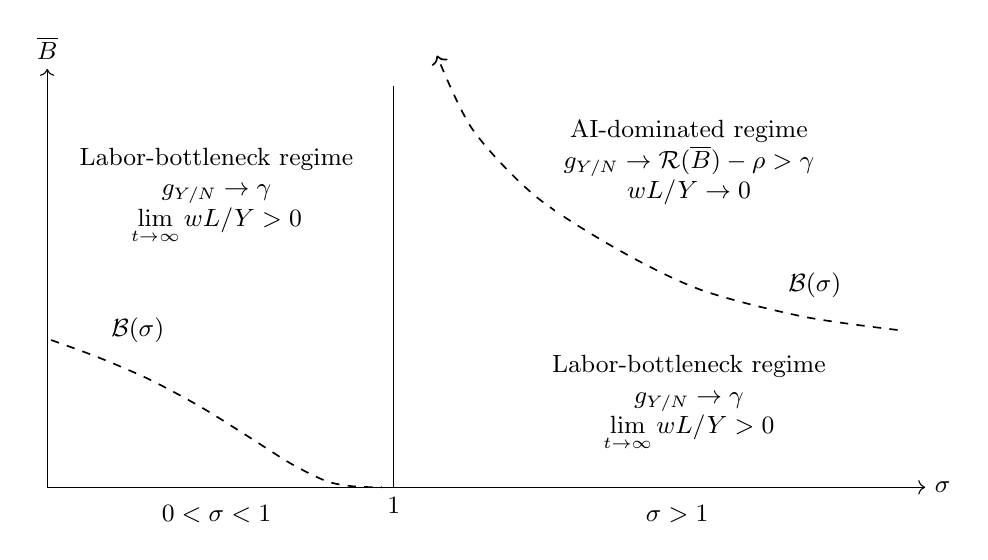
\begin{tikzpicture}[
 x=1.00cm,y=0.85cm,
 every node/.style={font=\small},
 regime/.style={align=center,inner sep=3pt,fill=white}
]
 \draw[->] (0,0) -- (11.15,0) node[right] {$\sigma$};
 \draw[->] (0,0) -- (0,6.25) node[above] {$\overline B$};
 \draw[semithick] (4.40,0) -- (4.40,6.00);
 \node[below] at (4.40,0) {$1$};
 \node[below] at (2.15,-0.12) {$0<\sigma<1$};
 \node[below] at (8.00,-0.12) {$\sigma>1$};

 % The complementary branch approaches zero as sigma approaches one
 % from below. It is not a continuation of the gross-substitutes branch.
 \draw[semithick,dashed]
  plot[smooth] coordinates
  {(0.05,2.20) (0.65,1.94) (1.30,1.61) (1.95,1.20)
   (2.55,0.76) (3.10,0.35) (3.55,0.09) (3.90,0.012)
   (4.25,0.001)};
 \node[regime] at (2.15,4.35)
  {Labor-bottleneck regime\\
   $g_{Y/N}\to\gamma$\\
   $\displaystyle\lim_{t\to\infty}wL/Y>0$};
 \node[regime] at (1.15,2.35) {$\mathcal B(\sigma)$};

 \draw[semithick,dashed,->]
  plot[smooth] coordinates
  {(10.80,2.35) (9.60,2.55) (8.30,2.95) (7.25,3.55)
   (6.20,4.35) (5.40,5.35) (4.95,6.45)};

 \node[regime] at (8.15,4.85)
  {AI-dominated regime\\
   $g_{Y/N}\to \mathcal R(\overline B)-\rho>\gamma$\\
   $wL/Y\to0$};
 \node[regime] at (8.15,1.25)
  {Labor-bottleneck regime\\
   $g_{Y/N}\to\gamma$\\
   $\displaystyle\lim_{t\to\infty}wL/Y>0$};
 \node[regime] at (9.75,3.02) {$\mathcal B(\sigma)$};
\end{tikzpicture}%
}
\caption{Growth regimes with an upper bound on AI efficiency. %For $0<\sigma<1$, $\overline B>\mathcal B(\sigma)$ is the condition for the positive-labor-share construction in Proposition~\ref{prop:rewrite-capped-complements-existence}. For $\sigma>1$, the curve separates the labor-bottleneck and AI-dominated equilibria in Proposition~\ref{prop:rewrite-capped-substitutes-labor-existence} and~\ref{prop:rewrite-capped-substitutes-existence}.
}
\label{fig:rewrite-frontier-regimes}
\end{figure}


Table~\ref{tab:rewrite-finite-existence} summarizes the four cases of Proposition~\ref{prop:rewrite-equilibrium-regimes}. For $\sigma>1$, an upper bound below $\mathcal B(\sigma)$ makes the return on capital at a vanishing labor share too low for capital and AI services to outgrow effective labor. Above the threshold, that return supports their faster growth along the AI-dominated equilibria. Across these equilibrium regimes, long-run wage growth exceeds $\gamma$ if and only if labor's income share converges to zero. %Proposition~\ref{prop:rewrite-output-wage-wedge} in Appendix~\ref{app:rewrite-proofs} derives the exact relationship between the wage-growth premium and the decline in labor's income share.


\begin{table}[H]
\centering
\caption{Long-run equilibrium characterization}
\label{tab:rewrite-finite-existence}
\small
\begin{tabular}{@{}cccccc@{}}
\toprule
Elasticity & AI efficiency bound & $\lim g_{Y/N}$ & $\lim g_w$ & $\lim wL/Y$ & $\lim r$ \\
\midrule
$0<\sigma<1$ & $\overline B>\mathcal B(\sigma)$ & $\gamma$ & $\gamma$ & Positive & $\rho+\gamma$ \\
$\sigma=1$ & Any finite $\overline B$ & $\gamma$ & $\gamma$ & $(1-\alpha)\omega_L$ & $\rho+\gamma$ \\
$\sigma>1$ & $\overline B<\mathcal B(\sigma)$ & $\gamma$ & $\gamma$ & Positive & $\rho+\gamma$ \\
$\sigma>1$ & $\overline B>\mathcal B(\sigma)$ & $\mathcal R(\overline B) -\rho$ & $\gamma+\frac{\mathcal R(\overline B)-\rho-\gamma}{\sigma}$ & Zero & $\mathcal R(\overline B)$ \\
\bottomrule
\end{tabular}
\end{table}


%I use this comparison as an economic regime threshold only for $\sigma>1$. For $\sigma<1$, $s_X\to1$ corresponds instead to AI services becoming scarce relative to effective labor. The condition $\overline B>\mathcal B(\sigma)$, or $\mathcal R(\overline B)>\rho+\gamma$, is then only a sufficient condition for the positive-labor-share construction in Proposition~\ref{prop:rewrite-capped-complements-existence}; it does not imply AI-dominated growth.


%Section~\ref{sec:rewrite-uncapped} studies the economy without an upper bound on AI efficiency. Those results require a separate equilibrium analysis.

\section{Competitive Equilibrium}
\label{sec:rewrite-competition}

I now replace the monopolistic developer with competitive AI suppliers.
This comparison separates the incentive to improve AI from the use of
technology already developed. I focus on $\sigma>1$, where both
labor-bottleneck and AI-dominated growth are possible. I first characterize
the competitive equilibrium and then compare it with the monopoly
equilibria in Section~\ref{sec:rewrite-regimes}.

\subsection{Characterization}
\label{subsec:rewrite-competitive-equilibrium}

Consider now the case where multiple AI suppliers have free access to the same efficiency $B$. Entry is free,
and any improvement becomes immediately available to every supplier,
without royalties or other compensation to its developer. There are no
research subsidies or publicly financed research. Suppliers and households
take prices and the common technology as given. Preferences, final-good
production, and the RSI technology remain unchanged.

Competition sets $p_X=1/B$. Since $X=BU$, revenue then exactly covers
inference compute: $p_XX=U$. Final-good firms continue to solve
problem~\eqref{eq:rewrite-final-firm-problem}, with production given by
equations~\eqref{eq:rewrite-output}--\eqref{eq:rewrite-ces}.
Their demand for AI services in equation~\eqref{eq:rewrite-ai-price}
then implies $U=(1-\alpha)s_XY$, since $X=B_0U$. The household continues to choose consumption and saving according to
the Euler equation~\eqref{eq:rewrite-euler} and the transversality
condition~\eqref{eq:rewrite-household-tvc}. Capital accumulation follows
the resource constraint~\eqref{eq:rewrite-resource} with $M=0$.
Competitive suppliers' optimality replaces
the monopolist's pricing, research, and shadow-price conditions.

As labor's income share vanishes, the net return on capital under
marginal-cost pricing approaches
\begin{equation}
 \mathcal R^{\mathrm{mc}}(B)
 =\alpha\left[(1-\alpha)B\,
 \omega_X^{\sigma/(\sigma-1)}\right]^{(1-\alpha)/\alpha}-\delta.
 \label{eq:rewrite-marginal-cost-return}
\end{equation}
Let $\mathcal B^{\mathrm{mc}}(\sigma)$ be the unique efficiency at which
$\mathcal R^{\mathrm{mc}}(\mathcal B^{\mathrm{mc}}(\sigma))=\rho+\gamma$.
Unlike the monopoly economy, the competitive economy cannot improve
from $B_0$ toward $\overline B$. Its long-run regime depends on the
efficiency inherited at the initial date.

\Needspace{24\baselineskip}
\begin{proposition}[Competitive equilibrium without private research]
\label{prop:rewrite-competitive-equilibrium}
Under the free-access arrangement described above, suppose $\sigma>1$.
For every $A_0,N_0,K_0>0$ and $0<B_0<\overline B$, there is a unique competitive equilibrium. At every date,
\begin{equation}
 M=0,\qquad B=B_0,\qquad p_{X}=1/B_0,\qquad \Pi=0.
 \label{eq:rewrite-competitive-no-research}
\end{equation}
Its long-run outcomes are as follows:
\begin{enumerate}[label=(\roman*),leftmargin=*,itemsep=0.5em]
\item If $B_0<\mathcal B^{\mathrm{mc}}(\sigma)$, labor remains a bottleneck:
\[
 g_{Y/N}\to\gamma,\qquad g_w\to\gamma,\qquad
 r\to\rho+\gamma,\qquad \lim_{t\to\infty}wL/Y>0.
\]
\item If $B_0>\mathcal B^{\mathrm{mc}}(\sigma)$, growth is AI-dominated:
\begin{gather}
 g_{Y/N}\to\mathcal R^{\mathrm{mc}}(B_0)-\rho>\gamma,\qquad
 g_w\to\gamma+
 \frac{\mathcal R^{\mathrm{mc}}(B_0)-\rho-\gamma}{\sigma}>\gamma,
 \label{eq:rewrite-competitive-ai-growth}\\
 r\to\mathcal R^{\mathrm{mc}}(B_0),\qquad wL/Y\to0.\nonumber
\end{gather}
\item At $B_0=\mathcal B^{\mathrm{mc}}(\sigma)$, both growth rates
converge to $\gamma$ and $r\to\rho+\gamma$, but $wL/Y\to0$.
\end{enumerate}
\end{proposition}
\begin{proof}
See Appendix~\ref{app:rewrite-proofs},
\hyperref[proof:rewrite-competitive-equilibrium]{Proof of
Proposition~\ref*{prop:rewrite-competitive-equilibrium}}.
\end{proof}

The absence of RSI does not eliminate AI-dominated growth. At fixed
efficiency, $X=B_0U$ can continue expanding through greater compute use.
When $B_0$ exceeds the competitive threshold
$\mathcal B^{\mathrm{mc}}(\sigma)$, capital and AI services
grow together faster than effective labor. This is the capital-accumulation
mechanism identified in Section~\ref{subsec:rewrite-equilibrium-existence},
now sustained without private research. Below the threshold, diminishing
returns bring the interest rate back to $\rho+\gamma$. Since $B=B_0$,
the competitive economy cannot escape this bottleneck through its own
research, even if the upper bound would permit much higher efficiency.
The equality case
is a boundary: capital per unit of effective labor grows without bound,
but its growth rate tends to zero, so the labor share vanishes without a
permanent growth premium.

AI-industry revenue remains distinct from profit. In the competitive
AI-dominated regime, $p_XX/Y\to1-\alpha$, just as under monopoly.
Here, however, all of that revenue pays for inference compute, and net
AI-industry profit is zero. A large AI revenue share therefore need not
represent monopoly rents.

\subsection{Comparison with monopoly}
\label{subsec:rewrite-monopoly-threshold}

I first compare the efficiency required under the two pricing rules,
holding the technology fixed. This isolates the effect of pricing from
the difference in research incentives.

\Needspace{12\baselineskip}
\begin{proposition}[Monopoly pricing and the AI-efficiency threshold]
\label{prop:rewrite-monopoly-threshold}
Suppose AI and labor are substitutes $(\sigma>1)$. Let
$\mathcal B(\sigma)$ and $\mathcal B^{\mathrm{mc}}(\sigma)$ denote the
AI-efficiency thresholds under monopoly pricing and marginal-cost
pricing, respectively.
These thresholds identify the efficiency needed for the return on
capital to reach $\rho+\gamma$ in the limit where labor's income share
vanishes. Monopoly pricing requires a higher AI efficiency:
\begin{equation}
 \mathcal B^{\mathrm{mc}}(\sigma)
 =(1-\alpha)\mathcal B(\sigma)<\mathcal B(\sigma).
 \label{eq:rewrite-marginal-cost-threshold}
\end{equation}
\end{proposition}
\begin{proof}
See Appendix~\ref{app:rewrite-proofs},
\hyperref[proof:rewrite-monopoly-threshold]{Proof of
Proposition~\ref*{prop:rewrite-monopoly-threshold}}.
\end{proof}

To understand why monopoly pricing raises the threshold, I compare the
same AI technology with the same capital and effective labor under the
two pricing rules. At marginal cost, AI services are cheaper, so final-good
firms use more of them and produce more with the same capital. This raises
the output--capital ratio and therefore the return on capital. For the
threshold comparison, I evaluate both returns as labor's income share
tends to zero. In this limit, monopoly pricing requires a higher AI
efficiency for the return on capital to reach the benchmark $\rho+\gamma$.
With $\alpha=0.33$, marginal-cost pricing reaches this benchmark at only
$67.0\%$ of the AI efficiency required under monopoly pricing.

Starting from the same initial state, the two economies need not retain
the same technology. Competitive efficiency remains at $B_0$, whereas
efficiency approaches $\overline B$ along the monopoly equilibria
characterized in Proposition~\ref{prop:rewrite-equilibrium-regimes}.
For example, if
\begin{equation}
 \mathcal B^{\mathrm{mc}}(\sigma)<B_0<\overline B<\mathcal B(\sigma),
 \label{eq:rewrite-competition-escapes-bottleneck}
\end{equation}
the competitive economy has AI-dominated growth, while any monopoly
equilibrium characterized by
Proposition~\ref{prop:rewrite-capped-substitutes-labor-existence}
remains labor-bottlenecked. This comparison applies to a nonempty set of
common initial states: choose
$\overline B\in(\mathcal B^{\mathrm{mc}}(\sigma),\mathcal B(\sigma))$
and $B_0$ sufficiently close to it in the monopoly existence construction.
The competitive equilibrium exists from each of those same states.

The efficiency gain from research must also be considered.
Conditional on both economies converging to AI-dominated
regimes, their limiting returns satisfy
\begin{equation}
 \mathcal R^{\mathrm{mc}}(B_0)\gtrless\mathcal R(\overline B)
 \quad\Longleftrightarrow\quad
 B_0\gtrless(1-\alpha)\overline B.
 \label{eq:rewrite-competitive-monopoly-growth-comparison}
\end{equation}
Equality holds on one side if and only if it holds on the other.
The same ordering applies to long-run output-per-worker and wage growth.
Thus, when both equilibria are AI-dominated, monopoly delivers faster
long-run growth if $B_0<(1-\alpha)\overline B$; competition delivers
faster growth if the inequality is reversed. The research-induced
efficiency gain must therefore be large enough to offset the monopoly
markup. This comparison is conditional on the existence of both
equilibrium trajectories from the same initial state. The competitive
existence result is global, but the monopoly construction in
Proposition~\ref{prop:rewrite-equilibrium-regimes} is local in initial
stocks. Equation~\eqref{eq:rewrite-competitive-monopoly-growth-comparison}
does not extend that existence result to initial states outside those
neighborhoods.

\subsection{Research incentives and policy}
\label{subsec:rewrite-competition-policy}

Holding $K$, $AL$, and $B$ fixed, marginal-cost pricing maximizes
$Y-X/B$ and leaves more resources available for consumption or capital
accumulation. In the free-access economy, however, it also removes the
private return to research. The comparison does not rank welfare:
that requires comparing consumption throughout the transition, including
the resource cost and future benefits of research under monopoly.

This raises a classic time-inconsistency problem \citep{kydlandprescott1977}.
A government may promise monopoly protection to encourage research, but
later wish to remove the markup once the technology has been developed.
Anticipating this policy reversal can weaken the developer's incentive to
invest in research. In the present setting, continued RSI makes the trade-off relevant
even after a valuable AI technology already exists: opening access to
that technology changes the rewards for improving it further.

An announced rule that ends monopoly protection at a specified efficiency
level is different from reneging on a promise. It nevertheless changes
the developer's problem. Without compensation, reaching that level would
remove future monopoly rents, potentially giving the developer an
incentive to delay reaching it. The threshold
$\mathcal B^{\mathrm{mc}}(\sigma)$ identifies the AI efficiency at which the
limiting return on capital under marginal-cost pricing reaches $\rho+\gamma$.
It does not identify the optimal time to end monopoly protection.
Choosing that time requires accounting for the
research response and comparing consumption paths under alternative rules.

\Needspace{3\baselineskip}
Patent buyouts offer a possible way to reward innovation without retaining
the monopoly markup. \citet{kremer1998} studies government purchases of
patents that are generally placed in the public domain. Applied here,
the idea would be to compensate the developer for the rights to an
existing AI technology and allow competing suppliers to use it.
Competitive supply at the same efficiency would require access to the
algorithms and model weights.
The buyout would also need a credible valuation and payment rule, a
source of financing, and arrangements to reward subsequent improvements.
Incentives for further development depend on
whether developers can appropriate its benefits. These issues are
particularly important for RSI, where today's technology is also an
input into tomorrow's research. I leave the design of such a policy,
including its effects on research and welfare, to an extension of the model.

\section{Equilibrium without an upper bound on AI efficiency}
\label{sec:rewrite-uncapped}

I now return to the monopoly economy, remove the upper bound on AI efficiency, and compare the three
substitution regimes. The RSI technology becomes
\begin{equation}
 \dot B=\chi(BM)^\eta.
 \label{eq:rewrite-uncapped-unit-law}
\end{equation}
All other primitives remain as in Section~\ref{sec:rewrite-model}.
In Definition~\ref{def:rewrite-equilibrium}, I set $\psi(B)=1$ and
$\psi'(B)=0$ and remove the upper restriction on $B$. Equilibrium still
requires finite allocations at every finite date, global agent optimality,
and both transversality conditions. %Removing the upper bound does not by itself imply that $B$ grows without bound.
%For any positive variable $V$, I write $g_V=\dot V/V$ for its growth rate.

The results differ in scope across substitution regimes. Under complementarity, long-run average output-per-worker growth cannot exceed the rate of labor-augmenting technological progress, even without an upper bound on AI efficiency. At unit elasticity, I give sufficient parameter restrictions for an analytically tractable balanced-growth equilibrium. Under substitution and sufficiently strong returns to research, the developer can make discounted net profit arbitrarily large even over a fixed finite horizon, ruling out an equilibrium with a finite-valued developer optimum.

\subsection{Complementarity}
\label{subsec:rewrite-uncapped-complements}

When $\sigma<1$, effective labor remains necessary even if AI becomes arbitrarily efficient. Equation~\eqref{eq:rewrite-ces} gives an upper bound for $Z$ and $Y$ which does not depend on $B$:
\begin{align}
 Z&\leq\omega_L^{\sigma/(\sigma-1)}AL,
 \label{eq:rewrite-uncapped-complements-z-bound}\\
 Y&\leq\omega_L^{\sigma(1-\alpha)/(\sigma-1)}
 K^\alpha(AL)^{1-\alpha}.
 \label{eq:rewrite-uncapped-complements-y-bound}
\end{align}

\Needspace{7\baselineskip}
\begin{proposition}[Production bounds under complementarity]
\label{prop:rewrite-uncapped-complements-bounds}
Let $0<\sigma<1$ and $\overline B=\infty$.
Along any feasible path satisfying the production equations~\eqref{eq:rewrite-output}
and~\eqref{eq:rewrite-ces}, labor-market clearing $L=N$ in
equation~\eqref{eq:rewrite-eq-labor},
and the resource constraint~\eqref{eq:rewrite-resource}, the following holds:
\begin{equation}
 \limsup_{t\to\infty}\frac1t
 \log\left(\frac{Y_t/N_t}{Y_0/N_0}\right)\leq\gamma.
 \label{eq:rewrite-uncapped-complements-growth-bound}
\end{equation}
%Neither $K$, $Y$, nor $B$ can become unbounded at a finite date.
\end{proposition}
\begin{proof}
See Appendix~\ref{app:rewrite-proofs},
\hyperref[proof:rewrite-uncapped-complements-bounds]{Proof of
Proposition~\ref*{prop:rewrite-uncapped-complements-bounds}}.
\end{proof}

%Thus a permanent growth rate of output per person above $\gamma$ is infeasible, although transitional growth can exceed it. %These are feasibility bounds, not an equilibrium-existence theorem. They also do not require $\eta<\alpha$: $0<\eta<1$ suffices to bound AI efficiency on a finite horizon once research expenditure is bounded by available resources.
Complementarity bounds long-run average output-per-worker growth despite RSI and the absence of an AI-efficiency upper bound. This does not prevent growth from temporarily exceeding $\gamma$.

%The monopoly matters for the limiting income shares. If its marginal cost $1/B$ tends to zero, the developer does not supply unlimited AI services. It approaches the quantity that maximizes revenue. The following conditional result states the implications without assuming that such an equilibrium has been constructed.

\Needspace{7\baselineskip}
\begin{proposition}[Long-run outcomes under complementarity without an AI efficiency upper bound]
\label{cond:rewrite-uncapped-complements-limits}
Suppose $0<\sigma<1$, $\overline B=\infty$, and an equilibrium satisfies
$B\to\infty$. Then
\begin{align}
 \frac KY&\to\frac{\alpha}{\rho+\gamma+\delta}>0,\qquad
 \frac CY\to1-\frac{\alpha(\delta+n+\gamma)}{\rho+\gamma+\delta}>0,
 \label{eq:rewrite-uncapped-complements-allocation-ratios}\\
 \frac UY&\to0,\qquad \frac MY\to0,
 \label{eq:rewrite-uncapped-complements-compute-shares}\\
 g_{Y/N}&\to\gamma,\qquad g_w\to\gamma,\qquad r\to\rho+\gamma,
 \label{eq:rewrite-uncapped-complements-rates}\\
 s_X&\to\frac{1-\sigma}{1-\alpha\sigma},
 \label{eq:rewrite-uncapped-complements-sx}\\
 \frac{wL}{Y}&\to\frac{\sigma(1-\alpha)^2}{1-\alpha\sigma}>0,
 \qquad
 \frac{p_XX}{Y}\to\frac{(1-\alpha)(1-\sigma)}{1-\alpha\sigma}>0.
 \label{eq:rewrite-uncapped-complements-income}
\end{align}
\end{proposition}
\begin{proof}
See Appendix~\ref{app:rewrite-proofs},
\hyperref[proof:rewrite-uncapped-complements-limits]{Proof of
Proposition~\ref*{cond:rewrite-uncapped-complements-limits}}.
\end{proof}

Conditional on $B\to\infty$, inference and research compute vanish as shares of output, not necessarily in levels. The AI industry nevertheless retains a positive revenue share.

%The limiting income shares follow from the static monopoly condition, equation~\eqref{eq:rewrite-monopoly-foc}. At positive limiting capital per unit of effective labor, $1/B\to0$ implies $e_X\to1$. Substituting into equation~\eqref{eq:rewrite-inverse-demand-elasticity} gives \eqref{eq:rewrite-uncapped-complements-sx}; equations~\eqref{eq:rewrite-wage} and~\eqref{eq:rewrite-ai-price} then give the income shares. The industry retains positive revenue even though its inference cost vanishes relative to output.

\subsection{Unit elasticity}
\label{subsec:rewrite-uncapped-unit-bgp}

At unit elasticity, production becomes
\begin{equation}
 Y=K^\alpha(AL)^{(1-\alpha)\omega_L}X^{(1-\alpha)\omega_X}.
 \label{eq:rewrite-uncapped-unit-elasticities}
\end{equation}
Consider a balanced-growth path (BGP) with positive constant $K/Y$, $C/Y$,
and $M/Y$. The AI-demand and
monopoly conditions, equations~\eqref{eq:rewrite-ai-price}
and~\eqref{eq:rewrite-monopoly-foc}, imply $U/Y=(1-\alpha)^2\omega_X^2$.
Along the BGP, $g_K=g_U=g_M=g_Y$. Substituting $X=BU$ into production,
equation~\eqref{eq:rewrite-uncapped-unit-elasticities}, and log-differentiating
this equation and the RSI technology in equation~\eqref{eq:rewrite-uncapped-unit-law}
yields
\begin{align}
 g_Y&=n+\gamma+\frac{\omega_X}{\omega_L}g_B,
 \label{eq:rewrite-uncapped-unit-production-growth}\\
 (1-\eta)g_B&=\eta g_Y.
 \label{eq:rewrite-uncapped-unit-research-growth}
\end{align}
The first relation describes how AI improvement raises production growth.
The second describes how expanding research resources sustain AI improvement.
Solving these relations gives candidate growth rates. The next proposition
establishes that they belong to an equilibrium.

\Needspace{7\baselineskip}
\begin{proposition}[An uncapped balanced-growth equilibrium and local convergence]
\label{prop:rewrite-uncapped-unit-bgp}
\label{prop:rewrite-uncapped-unit-local}
Suppose $\sigma=1$, $\overline B=\infty$, and
\begin{equation}
 \eta+\omega_X<1.
 \label{eq:rewrite-uncapped-unit-sufficient}
\end{equation}
\begin{enumerate}[label=(\roman*),leftmargin=*]
\item There is an equilibrium trajectory such that
\begin{align}
 g_{Y/N}=g_w& =\gamma+\frac{\eta\omega_X}{1-\eta-\omega_X}(n+\gamma),
 \label{eq:rewrite-uncapped-unit-wage-growth}\\
 r&=\rho+\gamma+\frac{\eta\omega_X}{1-\eta-\omega_X}(n+\gamma),
 \label{eq:rewrite-uncapped-unit-return}\\
 \frac{wL}{Y}&=(1-\alpha)\omega_L>0,
 \label{eq:rewrite-uncapped-unit-labor-share}\\
 g_B&=\frac{\eta(1-\omega_X)}{1-\eta-\omega_X}(n+\gamma).
 \label{eq:rewrite-uncapped-unit-efficiency-growth}
\end{align}
\item There is an open neighborhood of the initial condition
$(A_0,N_0,K_0,B_0)$ of the BGP in part (i) such that, from every initial
condition in that neighborhood, there exists an equilibrium trajectory
converging to the corresponding BGP in normalized variables.
\end{enumerate}
%Both agents attain finite-valued global optima; both transversality conditions hold.
\end{proposition}
\begin{proof}
See Appendix~\ref{app:rewrite-proofs},
\hyperref[proof:rewrite-uncapped-unit-bgp]{Proof of
Proposition~\ref*{prop:rewrite-uncapped-unit-bgp}}.
\end{proof}

Proposition~\ref{prop:rewrite-uncapped-unit-bgp} shows that RSI can sustain
permanently faster wage growth without a vanishing labor income share.
Equations~\eqref{eq:rewrite-uncapped-unit-wage-growth}
and~\eqref{eq:rewrite-uncapped-unit-labor-share} imply
$g_w=g_{Y/N}>\gamma$ while $wL/Y=(1-\alpha)\omega_L$ remains
constant and positive. Wages therefore keep pace with output per
worker. This contrasts with the regimes with an upper bound in
Proposition~\ref{prop:rewrite-equilibrium-regimes}, where a permanent
wage-growth premium occurs only in the AI-dominated regime and accompanies
a vanishing labor share. A declining labor share is therefore not a
necessary consequence of recursive self-improvement.

%Equations~\eqref{eq:rewrite-uncapped-unit-wage-growth} and~\eqref{eq:rewrite-uncapped-unit-efficiency-growth} quantify the two feedback loops. In the technological loop, a higher $B$ makes each unit of research compute more productive through $BM$. In the economic loop, better AI raises output, allowing more resources to be devoted to research. Along this BGP, the developer optimally chooses a positive constant $M/Y$, so research compute grows with output. Despite autonomous research, $g_B$ remains proportional to the growth rate of effective labor, $n+\gamma$. Human labor no longer enters the RSI technology, but at unit elasticity itremains essential to final-good production. 
Growth in effective labor expands the resources available for research, which raises $B$ and further
expands output. The common denominator $1-\eta-\omega_X$ captures
this reinforcement: a higher $\eta$ strengthens the research feedback,
while a higher $\omega_X$ makes output growth more responsive to AI
improvement.
A related dependence appears in \citet{jones1995}, where long-run growth
depends on an expanding research workforce. Here, effective labor supports
research indirectly through production, rather than entering the RSI
technology itself.

\subsection{Substitution}
\label{subsec:rewrite-uncapped}

With $\sigma>1$, Proposition~\ref{prop:rewrite-equilibrium-regimes}
establishes AI-dominated equilibria whose limiting interest rate is
$\mathcal R(\overline B)$, which grows without bound as
$\overline B\to\infty$. %This contrasts withpropositions \ref{prop:rewrite-capped-complements-existence} and \ref{prop:rewrite-uncapped-complements-bounds}: undercomplementarity, growth is bounded in the long run by the labor-augmenting technological progress.
The same function also bounds the equilibrium interest rate
without an efficiency upper bound:
\begin{equation}
 r_t\geq\mathcal R(B_t)%,\qquad \sigma>1
 .
 \label{eq:rewrite-uncapped-dated-return-bound}
\end{equation}
To see this, combine equations~\eqref{eq:rewrite-ai-output-limit},
\eqref{eq:rewrite-composite-ai-limit}, and~\eqref{eq:rewrite-output-capital-limit}
before taking the limit $s_X\to1$:
\begin{equation}
 \frac YK=
 \left[B(1-\alpha)\omega_X^{\sigma/(\sigma-1)}
 (1-e_X)s_X^{-1/(\sigma-1)}\right]^{(1-\alpha)/\alpha}.
 \label{eq:rewrite-substitutes-dated-output-capital}
\end{equation}
For fixed $B$ and $\sigma>1$, this expression decreases with $s_X$ and
approaches its lower limit as $s_X\to1$.
%\footnote{Using
%$e_X=(1-s_X)/\sigma+\alpha s_X$ from
%equation~\eqref{eq:rewrite-inverse-demand-elasticity},
%\[
% \frac{\mathrm d\log[(1-e_X)s_X^{-1/(\sigma-1)}]}
% {\mathrm d\log s_X}
% =\frac{(\sigma-2)(1-\alpha\sigma)s_X-(\sigma-1)}
% {\sigma(\sigma-1)(1-e_X)}<0.
%\]
%The denominator is positive for $\sigma>1$. The numerator is affine in
%$s_X$ and negative at both endpoints: $-(\sigma-1)$ at zero and
%$-[1-\alpha+\alpha(\sigma-1)^2]$ at one.}
Substitution into $r=\alpha Y/K-\delta$ gives
inequality~\eqref{eq:rewrite-uncapped-dated-return-bound}.
Thus $\mathcal R(B)$ is the lowest return compatible with the production
and monopoly conditions at that efficiency level, attained in the
zero-labor-share limit. If $B$ grows without bound along a trajectory, inequality~\eqref{eq:rewrite-uncapped-dated-return-bound} requires
$r\to\infty$ and $Y/K\to\infty$. Production also gives
$Z/Y=(Y/K)^{\alpha/(1-\alpha)}\to\infty$, while the Euler
equation~\eqref{eq:rewrite-euler} requires
$g_{C/N}=r-\rho\to\infty$.

\citet{davidsonetal2026} show that technological and economic feedback loops
can overcome diminishing returns to research and generate \emph{hyperbolic
growth}, with variables diverging at a finite date. This \emph{finite-time
singularity} is stronger than an indefinitely increasing growth rate.
Their benchmark fixes saving and factor-allocation shares; I therefore
cannot apply its explosion conditions directly to the optimal choices
studied here.

Under Definition~\ref{def:rewrite-equilibrium}, a finite-time singularity
cannot constitute an infinite-horizon equilibrium, which requires finite
allocations at every finite date. The return bound in
equation~\eqref{eq:rewrite-uncapped-dated-return-bound} does not determine
whether divergence occurs in finite or infinite time. The following
proposition instead shows that, when research returns are
sufficiently strong, the developer can make discounted net profit arbitrarily
large even over a fixed finite horizon. This is an unbounded optimization
problem, not a trajectory that attains infinite profit in finite time.

%The developer's problem distinguishes the cases $\eta<\alpha$ and $\eta>\alpha$.

\Needspace{8\baselineskip}
\begin{proposition}[Research expenditure and the developer's value]
\label{prop:rewrite-research-scale}
Suppose $\sigma>1$, $\overline B=\infty$ and $0<\alpha <\eta<1$.
Fix any $B_0>0$, any finite horizon $T>0$, positive continuous paths of
$K,A,L$, and an integrable interest-rate path. For the developer's
problem~\eqref{eq:rewrite-developer-reduced} restricted to $[0,T]$%:
%\begin{enumerate}[label=(\roman*),leftmargin=*]
%\item If $\eta<\alpha$, discounted net profit is bounded above over all
%research plans and tends to minus infinity as total research expenditure
%over $[0,T]$ tends to infinity.
%\item If $\eta>\alpha$, the developer can make discounted net profit arbitrarily large. Consequently, there is no infinite-horizon equilibrium
%with a finite-valued developer optimum.
%\end{enumerate}
, the developer can make discounted net profit arbitrarily large.
\end{proposition}
\begin{proof}
See Appendix~\ref{app:rewrite-proofs},
\hyperref[proof:rewrite-research-scale]{Proof of
Proposition~\ref*{prop:rewrite-research-scale}}.
\end{proof}

%When $\eta<\alpha$, research costs eventually dominate profit gains on a fixed horizon. When $\eta>\alpha$, expanding early research makes the gains outgrow the cost. Each deviating plan uses finite research expenditure and keeps AI efficiency finite on every finite interval. The obstruction is therefore an unbounded objective, not a finite-time singularity.

%The first case motivates the choice $\eta=0.20<\alpha=0.33$ in Section~\ref{sec:rewrite-quantitative}: it avoids this unbounded-payoff mechanism even without an efficiency cap. This is a modeling restriction, not an estimate of $\eta$. With a finite upper bound, $\eta<\alpha$ is not needed to bound the developer's finite-horizon value. Part (i) does not establish an infinite-horizon equilibrium without an upper bound. At $\eta=\alpha$, comparing the growth orders of benefits and costs alone is inconclusive.

% BEGIN COMMENTED PREVIOUS SECTION 5.3 (2026-09-13)
% Preserved verbatim below, with one comment prefix per line.
% Its proof file is retained but its input in appendix.tex is commented.
% \subsection{Substitution: unbounded returns and equilibrium existence}
% \label{subsec:rewrite-uncapped}
%
% Proposition~\ref{prop:rewrite-equilibrium-regimes} does not establish equilibrium existence without an upper bound for AI efficiency. I first fixed $\overline B$ and characterized an equilibrium for initial conditions near the steady state. Increasing $\overline B$ afterward differs from setting $\overline B=\infty$ at the outset. For $\sigma>1$, the limiting growth and interest rates of the AI-dominated equilibria become unbounded as $\overline B\to\infty$. This divergence is not a proof of a finite-time singularity or of equilibrium nonexistence in the uncapped economy.
%
% Without an upper bound, recursive improvement can make the developer's objective unbounded: higher $B$ raises both operating profit and research productivity. If $\sigma>1$ and $\eta>\alpha$, there is no uncapped equilibrium with a finite-valued developer optimum, as established in Proposition~\ref{prop:rewrite-research-scale} in Appendix~\ref{app:rewrite-proofs}. Expanding early research makes discounted net profit arbitrarily large on a fixed finite horizon. The developer can then resume any proposed continuation of research spending with higher AI efficiency and no lower operating profit. Thus every candidate with a finite value admits a profitable deviation. This failure of optimality does not require a finite-time singularity: each deviating plan uses finite research expenditure and keeps $B$ finite on every finite horizon. %Financing cannot resolve an unbounded objective or create the real resources used in research: equation~\eqref{eq:rewrite-eq-kdot} requires research compute to compete with consumption, inference compute, and physical investment.
%
% If $\eta<\alpha$ and $\sigma>1$, the same proposition gives a finite truncated value and shows that research costs eventually outgrow the benefits of increasing expenditure on a fixed horizon. This result takes the paths of capital, effective labor, and interest rates as given. It rules out that particular unbounded-payoff argument, without establishing an uncapped infinite-horizon equilibrium. Neither existence nor general nonexistence is established for this parameter range. On its own, this fixed-horizon result does not establish or rule out a finite-time singularity, which would violate the requirement of finite, feasible allocations at every date in Definition~\ref{def:rewrite-equilibrium}.
%
% The equilibrium in Section~\ref{subsec:rewrite-uncapped-unit-bgp} shows that
% unbounded AI efficiency is compatible with equilibrium at unit elasticity.
% It does not resolve existence for $\sigma>1$.
%
% At $\eta=\alpha$, the finite-horizon benefit and cost terms have the same
% order, so their coefficients determine whether that particular
% unbounded-payoff argument applies. Proposition~\ref{prop:rewrite-research-scale}
% does not settle equilibrium existence at this boundary.
%
% The return function derived in Section~\ref{subsec:rewrite-return-threshold}
% also gives a bound that holds at every date. For $\sigma>1$, the production
% and monopoly conditions imply
% \begin{equation}
%  r_t\geq\mathcal R(B_t).
%  \label{eq:rewrite-uncapped-dated-return-bound}
% \end{equation}
% The proof below derives this inequality without assuming $s_X\to1$ or
% $B\to\infty$. Thus, if AI efficiency grows without bound, the interest
% rate must do so too. Once $B_t>\mathcal B(\sigma)$, the Euler equation
% also gives $g_{C/N}=r_t-\rho>\gamma$. Unlike a comparison of long-run
% equilibria with different upper bounds, these are restrictions on a single
% trajectory.
%
% The literature suggests how to connect this return bound to a finite-time
% explosion. \citet{nordhaus2021} emphasizes the role of substitution, and
% \citet{davidsonetal2026} show how technological and capital-accumulation
% feedback can jointly overcome diminishing returns in research. Their
% benchmark holds saving and factor-allocation shares fixed; its discussion
% of endogenous saving draws on \citet{trammellkorinek2023}. I cannot apply
% its explosion theorem directly to the present model's optimal allocations.
% Instead, I use a comparison argument that allows investment shares to vary.
%
% \Needspace{7\baselineskip}
% \begin{proposition}[Investment restrictions without an efficiency upper bound]
% \label{prop:rewrite-uncapped-substitutes-explosion}
% Let $\sigma>1$, $\overline B=\infty$, $0<\alpha<1$, and $0<\eta<1$.
% No equilibrium in Definition~\ref{def:rewrite-equilibrium} can satisfy
% either of the following conditions:
% \begin{enumerate}[label=(\roman*),leftmargin=*,itemsep=0.4em]
% \item Both gross capital investment and research expenditure remain
% bounded below by positive shares of output. That is, there exist constants
% $\iota,\mu>0$ and a finite date $t_0$ such that
% \begin{equation}
%  \frac{\dot K_t+\delta K_t}{Y_t}\geq\iota,
%  \qquad \frac{M_t}{Y_t}\geq\mu
%  \qquad\text{for every }t\geq t_0.
% \label{eq:rewrite-uncapped-investment-floors}
% \end{equation}
% \item Both investment shares converge to finite limits:
% \begin{equation}
%  \lim_{t\to\infty}\frac{\dot K_t+\delta K_t}{Y_t}
%  \quad\text{and}\quad
%  \lim_{t\to\infty}\frac{M_t}{Y_t}
%  \quad\text{both exist and are finite.}
%  \label{eq:rewrite-uncapped-convergent-investment}
% \end{equation}
% These limits need not be positive; zero limiting shares are also excluded.
% \end{enumerate}
% \end{proposition}
% \begin{proof}
% See Appendix~\ref{app:rewrite-proofs},
% \hyperref[proof:rewrite-uncapped-substitutes-explosion]{Proof of
% Proposition~\ref*{prop:rewrite-uncapped-substitutes-explosion}}.
% \end{proof}
%
% In part (i), the constants $\iota$ and $\mu$ are lower bounds on expenditure shares,
% not additional parameters or imposed saving rules. The shares need not be
% constant or converge, and the proposition assumes neither $B\to\infty$
% nor $s_X\to1$. Persistent investment first prevents capital and output
% from disappearing and keeps research positive. AI efficiency must then
% eventually exceed every finite level. The return bound from Section~
% \ref{subsec:rewrite-return-threshold} makes depreciation negligible
% relative to investment and strengthens the feedback between capital and
% research. The proof obtains $\dot B\geq c_B B^{1/\alpha}$ for some
% constant $c_B>0$ at sufficiently late dates. Since $1/\alpha>1$, this
% inequality contradicts finite AI efficiency at every finite date. The
% argument works whether $\eta<\alpha$, $\eta=\alpha$, or $\eta>\alpha$.
%
% Part (ii) uses optimality to exclude the possibility that convergent
% investment shares avoid this feedback by tending to zero. If $B\to\infty$,
% the household Euler equation and feasibility imply
% \begin{equation}
%  \limsup_{t\to\infty}\frac{\dot K_t+\delta K_t}{Y_t}\geq\alpha.
%  \label{eq:rewrite-uncapped-capital-limsup}
% \end{equation}
% Thus a convergent capital-investment share cannot be zero. The research
% choice and the developer's transversality condition then rule out a zero
% limiting research share. The proof also excludes a finite limiting $B$
% under the same convergence hypothesis; divergence of $B$ is not assumed.
% Convergence of these two shares is weaker than balanced growth: neither
% constant growth rates nor convergence of their derivatives is required.
%
% Section~\ref{sec:rewrite-regimes} therefore supplies a key inequality for
% the proof, but not both investment bounds. Along its AI-dominated
% equilibria, for each fixed finite $\overline B$,
% \begin{equation}
%  \frac{\dot K+\delta K}{Y}
%  \longrightarrow
%  \frac{\alpha[n+\mathcal R(\overline B)-\rho+\delta]}
%  {\mathcal R(\overline B)+\delta}>0,
%  \qquad \frac MY\longrightarrow0.
%  \label{eq:rewrite-capped-investment-limits}
% \end{equation}
% The capital-investment limit follows from the limiting growth and return
% in Proposition~\ref{prop:rewrite-capped-substitutes-existence}; the research
% limit follows from the finite limiting level of $M$ in equation~
% \eqref{eq:rewrite-ai-terminal-values} in its proof. Raising the upper
% bound cannot turn these zero limiting research shares into a positive
% uniform lower bound. This does not imply that research shares vanish
% without an upper bound: that economy has a different research law.
%
% The developer's
% research condition~\eqref{eq:rewrite-research-foc}, costate
% equation~\eqref{eq:rewrite-costate}, and transversality
% condition~\eqref{eq:rewrite-developer-tvc} imply the necessary identity
% \begin{equation}
%  M_t^{1-\eta}=\eta\chi\int_t^\infty
%  \exp\left(-\int_t^s r_v\,\dd v\right)
%  U_s B_s^{\eta-1}\,\dd s.
%  \label{eq:rewrite-uncapped-research-pv}
% \end{equation}
% It equates current research incentives to future discounted savings in
% inference costs.\footnote{Write $P=M^{1-\eta}=\chi\eta qB^\eta$.
% Differentiating the research condition and using the uncapped costate
% equation gives $\dot P=rP-\eta\chi UB^{\eta-1}$.
% For $D_t=\exp(-\int_0^t r_v\,\dd v)$, the developer's transversality
% condition implies $D_tP_t\to0$, since
% $D_tP_t=\chi\eta(D_tq_tB_t)B_t^{\eta-1}$ and $B_t\geq B_0>0$.
% Integrating $\mathrm d(DP)/\mathrm dt$ proves
% equation~\eqref{eq:rewrite-uncapped-research-pv}.}
% Positive research at every date does not establish a positive lower bound
% on $M/Y$. Likewise, a higher interest rate raises consumption growth
% through the Euler equation but does not by itself determine how saving
% is divided between physical capital and research. These incentive
% conditions must be analyzed jointly with feasibility, as in the proof of
% part (ii). Any remaining equilibrium candidate must have investment shares
% that do not both converge and cannot both stay above positive lower bounds.
% This restriction does not establish that such a candidate exists. The result
% is not yet a proof of general equilibrium nonexistence for $\eta\leq\alpha$:
% paths with nonconvergent investment shares remain to be analyzed.
% END COMMENTED PREVIOUS SECTION 5.3

\section{Numerical simulations}
\label{sec:rewrite-quantitative}

\subsection{Parameters and initial conditions}
\label{subsec:rewrite-rsi-activation}

In this section, I compare the transitional dynamics across four parameter configurations corresponding to the cases in Proposition~\ref{prop:rewrite-equilibrium-regimes}. I study an unanticipated activation of RSI at date zero. Before date zero, the economy already uses AI production services, but AI efficiency is fixed at $B_0$. For the chosen value of $B_0$, each economy starts on a labor-bottleneck balanced growth path. I compute this path with the research productivity parameter $\chi$ equal to zero to obtain the corresponding initial capital stock $K_0$ for each parameter configuration. Setting $\chi=0$ rules out improvements in AI efficiency, not the expansion of AI services through inference compute $U$. By treating activation as unanticipated, I exclude the advance adjustment of consumption and saving emphasized in the technology-news literature reviewed by \citet{beaudryportier2014}.

I compare four economies with $\sigma=0.9,1.0,1.1,1.5$, holding all other parameters and the initial values $A_0$, $N_0$, and $B_0$ fixed. For each economy, I choose $K_0$ to place it on its pre-RSI balanced growth path. In particular, for each elasticity, I choose the pre-event capital stock to satisfy
\begin{equation}
 r_0=\rho+\gamma,\qquad
 \frac{K_0}{Y_0}=\frac{\alpha}{\rho+\gamma+\delta}=3.30.
 \label{eq:rewrite-rsi-initial-ratio}
\end{equation}
This setup guarantees that $Y$, $X$, $U$, $w$, $r$, and $p_X$ behave continuously rather than jumping at date zero.

Table~\ref{tab:rewrite-rsi-parameters} reports the parameter values and initial stocks used for the simulations. I use standard values for $\alpha$, $\delta$, and $\rho$, while $n$ and $\gamma$ are guided by long-run population and productivity projections. The AI production weight $\omega_X=0.10$ and research exponent $\eta=0.20$ are illustrative choices, not empirical estimates. I choose them to satisfy $\omega_X+\eta<1$, the condition for the uncapped unit-elastic balanced-growth equilibrium in Proposition~\ref{prop:rewrite-uncapped-unit-bgp}; this is not a requirement for the simulations with an upper bound considered here. The common upper bound on AI efficiency satisfies $\mathcal B(1.5)<\overline B<\mathcal B(1.1)$. Thus, AI and labor are substitutes in both the $\sigma=1.1$ and $\sigma=1.5$ cases, but only the latter converges to the AI-dominated regime.

I study two levels of research productivity for each of the four elasticities of substitution. They both led to the same long-run growth rates in all variables, but differ in the speed at which growth accelerates once RSI becomes available. In the first one, higher-productivity scenario, $\chi$ is equal to 7.5. In the second one,  the lower-productivity scenario, $\chi$ is equal to 1.5. These are also illustrative choices, but their contrast show how different parameter values can lead to significant differences in the short-run impact of AI.

%In Equation~\eqref{eq:rewrite-rsi-initial-ratio}, $Y_0$ is obtained from the production and monopoly conditions with AI already present. Thus $K_0$ differs across elasticities, while the initial capital--output ratio and interest rate are common. With $A_0=N_0=1$ and the common $B_0$, the four capital stocks are approximately $3.434$, $4.649$, $5.037$, and $5.505$. These are calibrated alternative economies, not different outcomes of introducing AI into one economy with the same capital stock. The ratio is a theoretical BGP reference, not an exact empirical fit: the PWT 11.0 comparison yields a 2023 current-price capital--output ratio of about $3.61$ for the covered world sample and $3.42$ for the United States, with capital definitions that differ from the one-good model \citep{pwt110}.

% Edit Table 2 here: formatting, all rows, and notes are in this file.
% Display values only; this file does not set simulation inputs.
\begin{table}[H]
\centering
\caption{Simulation parameters and initial stocks}
\label{tab:rewrite-rsi-parameters}
\small\setstretch{1.0}
\setlength{\tabcolsep}{4pt}
\renewcommand{\arraystretch}{1.14}
\begin{tabular}{P{0.08\textwidth}P{0.12\textwidth}P{0.30\textwidth}P{0.36\textwidth}}
\toprule
Symbol & Value & Interpretation & Source\\
\midrule
$\alpha$ & 0.33 & Capital share & Standard calibration value.\\
$\delta$ & 0.05 & Depreciation rate & Standard calibration value.\\
$\rho$ & 0.04 & Discount rate & Standard calibration value.\\
$n$ & 0.003 & Population growth rate & Rounded constant-rate approximation to the UN 2024--2100 world projection \citep{unwpp2024}.\\
$\gamma$ & 0.01 & Growth of labor-augmenting technology & OECD labor-productivity projections \citep{oecdlongrun2025}.\\
$\eta$ & 0.20 & Research exponent & Illustrative.\\
%$(\omega_X,\omega_L)$ & (0.10, 0.90) & AI production and effective-labor weights & Illustrative.\\
$\omega_X$ & 0.10 & AI production weight & Illustrative.\\
$\omega_L$ & 0.90 & Effective-labor weight & $1-\omega_X$.\\
$\chi$ & 7.5 (higher);\newline 1.5 (lower) & Research productivity after activation & Illustrative.\\
$\sigma$ & 0.90;\newline 1.00;\newline 1.10;\newline 1.50. & Elasticity of substitution & Illustrative.\\
$\overline B$ & 1,361 & AI-efficiency upper bound & $1.10 \times \mathcal B(1.50)$.\\
\midrule
%$A_0,N_0$ & 1; 1 & Initial technology and population & Normalizations.\\
$A_0$ & 1 & Initial labor-efficiency units & Normalization.\\
$N_0$ & 1 & Initial population & Normalization.\\
$B_0$ & 13.6 & Initial AI efficiency & $0.01 \times \overline B$.\\
$K_0$ & 3.43;\newline 4.65;\newline  5.04;\newline 5.50. & Initial capital & Adjusted to match $K_0/Y_0 =3.30$, the pre-RSI balanced growth path ratio.\\
%$K_0/Y_0$ & 3.30 & Initial capital--output ratio & Derived from the pre-RSI balanced growth path.\\
\bottomrule
\end{tabular}
\par\vspace{4pt}
%\parbox{0.98\textwidth}{\footnotesize\emph{Notes:} %Rates are annual. Values are rounded for display; the simulations retain their original precision. $L_0=N_0$. %Initial consumption $C_0$ and the developer's shadow value $q_0$ are selected endogenously by the BVP for each path, not supplied as inputs. $K_0/Y_0$ is a derived ratio, measured in years of date-zero output, not an additional parameter. Lists of four ratios follow the displayed order of $\sigma$.}
\end{table}



%Before activation, consumption satisfies
%\begin{equation}
% C(0^-)=Y_0-U_0-(\delta+n+\gamma)K_0>0.
% \label{eq:rewrite-rsi-pre-consumption}
%\end{equation}
%Only $K_0$ and $B_0$, together with the exogenous $A_0,N_0$, are inherited by the post-event equilibrium. The BVP selects $C(0^+)$ and $q(0^+)$ anew. 
%The pre-event BGP requires an unanticipated activation: announcing RSI earlier would generally change saving and consumption before date zero, as in the technology-news mechanisms reviewed by \citet{beaudryportier2014}.

%Unlike the scenario in \citet{jonestonetti2026}, where endogenous automation is already underway, this exercise studies an unanticipated activation of RSI and so subsequent AI-efficiency improvements are endogenous. However, the exercise omits the costs of expanding compute capacity as in \citep{erdiletal2025gate} and the complementary intangible investment studied by \citet{brynjolfssonrocksyverson2021}. Those mechanisms can delay adjustment or measured productivity gains. 

I do not model a separate stock of computing hardware or the costs of
rapidly expanding it. \citet{erdiletal2025gate} incorporate adjustment costs
for compute capacity and other physical capital. Introducing such frictions
could change the initial reallocation of resources and the timing of the
transition shown here.

Appendix~\ref{app:rewrite-algorithm}
describes the algorithm used to find the equilibrium and presents the links to replication files.

\subsection{Higher research productivity}
\label{subsec:rewrite-rsi-half-decline}

I first ask how research, consumption, and capital accumulation respond
when RSI becomes available under an existing monopoly, and how this
adjustment differs across economies approaching the two long-run regimes.
I compare the four elasticities under relatively high research
productivity, $\chi=7.5$. Research productivity
affects the transition, but not the limiting growth rates characterized in
Section~\ref{sec:rewrite-regimes}. All four economies inherit the pre-RSI
balanced growth paths described in Section~\ref{subsec:rewrite-rsi-activation}.
Table~\ref{tab:rewrite-rsi-parameters} reports their common parameters and
elasticity-specific initial capital stocks. I examine quantities first,
then wages and prices, and finally income shares.

% The generated numerical digest in rsi_chi_7_5_results.tex is retained,
% but not input here: editorial prose is organized around the three figures.
% Source: numerical_rewrite/rsi_chi_7_5/{summary,figure_manifest}.json.
I use Figure~\ref{fig:rewrite-rsi-half-accumulation} to present the annual growth rates of output, AI production services, and capital per unit of effective labor: $Y/(AL)$, $X/(AL)$, and $K/(AL)$. Zero therefore means that the corresponding aggregate grows at the same rate as effective labor, $n+\gamma$. The upper row shows two pre-event years and the first ten years after RSI activation. The lower row follows the same variables from year 10 to year 500. Throughout the three figures, green dashed, black solid, orange dotted, and blue dash-dotted lines denote $\sigma=0.90,1,1.10,1.50$, respectively. The vertical line marks RSI activation, and black dotted horizontal lines mark the analytical
limits for $\sigma=1.50$. %Vertical scales differ across time windows.

\begin{figure}[H]
 \centering
 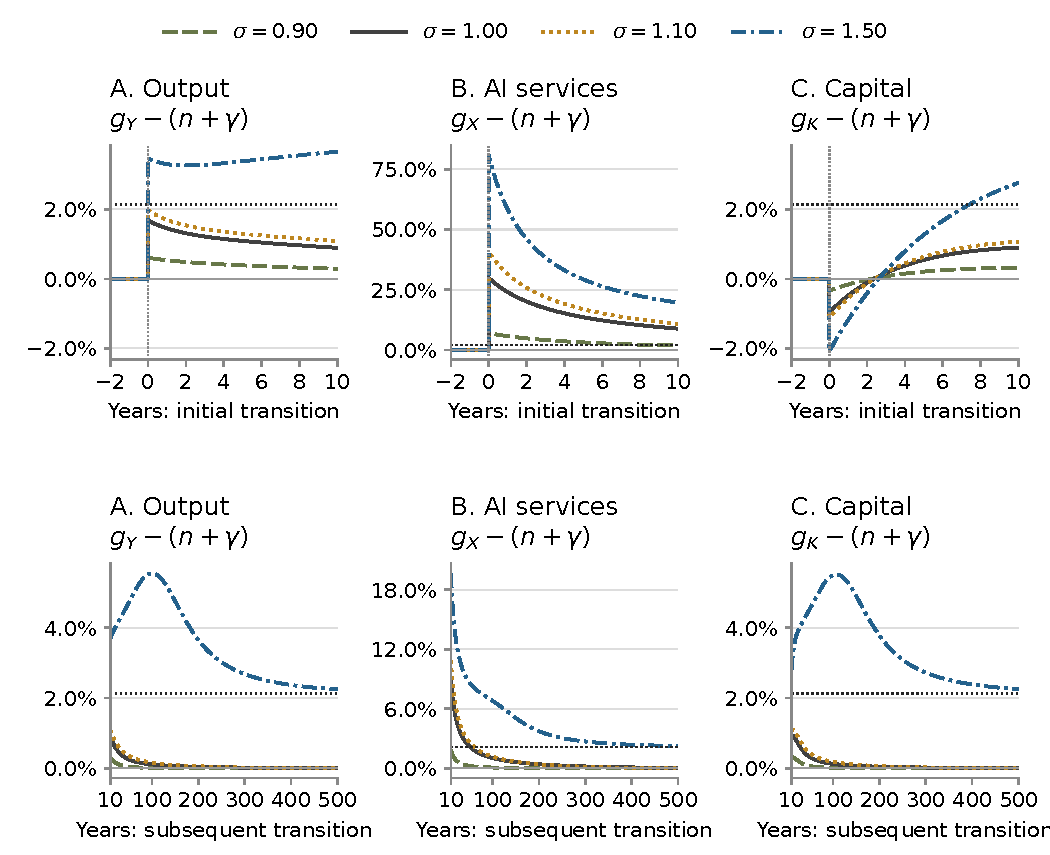
\includegraphics[width=\textwidth]{figures_rewrite/equilibrium_rsi_chi_7_5_accumulation_growth_windows.pdf}
 \caption{Higher research productivity ($\chi=7.5$): growth of output,
 AI production services, and capital per unit of effective labor. Rates
 are instantaneous annual rates. The upper row shows two pre-event years
 and years 0--10; the lower row shows years 10--500. Panels A and C share
 a scale within each row. The vertical line marks RSI activation.}
 \label{fig:rewrite-rsi-half-accumulation}
\end{figure}


The top row of Figure~\ref{fig:rewrite-rsi-half-accumulation} shows that AI services respond much more strongly than output. At $\sigma=1.50$, $X/(AL)$ initially grows at $80.8\%$ per year, whereas $Y/(AL)$ grows at $3.5\%$. Research begins to raise $B$, allowing more services to be obtained from compute through $X=BU$. Final production cannot expand at the same rate because it also requires capital and labor. Initial growth of $Y/(AL)$ is smaller at the other elasticities, reaching only $0.6\%$ at $\sigma=0.90$. The third panel shows the capital response: capital per unit of effective labor, $K/(AL)$, falls in every case. Households increase consumption at RSI activation while the developer starts spending on research. The resource constraint thus requires lower investment in physical capital. Capital accumulation
subsequently recovers as output expands and as the marginal product of capital increases.

The bottom row of Figure~\ref{fig:rewrite-rsi-half-accumulation} separates temporary growth gains from permanent ones. At $\sigma=0.90,1,1.10$, all three normalized growth rates decline
toward zero. This is the labor-bottleneck outcome in
Proposition~\ref{prop:rewrite-equilibrium-regimes}: output per worker eventually grows at $\gamma=1.0\%$. At $\sigma=1.50$, output and capital
growth instead rise further before declining toward their long-run values.
As explained in Section~\ref{subsec:rewrite-equilibrium-existence},
sufficient substitution and a sufficiently high efficiency bound allow
capital and inference compute to expand together without being limited
by effective-labor growth. Their limiting growth rates exceed effective-labor growth by $2.1$ percentage points; effective labor itself grows at $1.3\%$ per year.

I next examine wages and prices in Figure~\ref{fig:rewrite-rsi-half-prices}. The figure shows annual wage growth $g_w$, the annual net interest rate $r$, and the level of $p_X$ in final-good units on a logarithmic scale. The top panels present the short-run dynamics and the bottom panels present the long-run dynamics. Wage growth increases in all four economies, but the initial response is not ordered monotonically by substitutability: the immediate increase is larger at $\sigma=1$ than at $\sigma=1.50$. Wage growth in the highest-elasticity case soon surpasses the other cases. After the initial jump, wage growth declines in the labor-bottleneck cases but continues to rise in the AI-dominated case. Meanwhile, the interest rate starts at $5.0\%$ in every case and then rises as output initially outpaces capital. The higher return accompanies faster consumption-per-person growth, as required by the Euler condition in Equation~\eqref{eq:rewrite-euler}. A related mechanism underlies \citet{chowhalperinmazlish2026}, who link faster expected consumption growth to higher long-term real interest rates. Meanwhile, $p_X$ falls continuously as AI efficiency improves. %The pricing condition \eqref{eq:rewrite-eq-monopoly} links the price to the compute cost per service, $1/B$, and the markup. At unit elasticity the markup is constant, so the price falls in inverse proportion to $B$; its decline over the first 27 months is $39.6\%$, an outcome rather than a calibration target.

The bottom row of Figure~\ref{fig:rewrite-rsi-half-prices} shows the longer adjustment of wage growth, the interest rate, and the AI-service price. The three labor-bottleneck economies return toward wage growth of $1.0\%$ and an interest rate of $5.0\%$. At $\sigma=1.50$, both rates rise above their long-run values before declining. Equation~\eqref{eq:rewrite-substitutes-wage-growth} gives limiting wage growth of $2.4\%$, below output-per-worker growth of $3.1\%$ but above labor-augmenting technological progress of $1.0\%$. Meanwhile, the interest rate tends to $\mathcal R(\overline B)=7.1\%$, above its pre-RSI level. %At year 500, the corresponding wage growth and interest rate are still $2.5\%$ and $7.2\%$. The price approaches a positive level in every case, rather than falling forever at a constant proportional rate. In the AI-dominated limit, $s_X\to1$ and $e_X\to\alpha$, so the pricing condition gives $p_X\to1/[(1-\alpha)\overline B]\simeq0.00110$.

\begin{figure}[H]
 \centering
 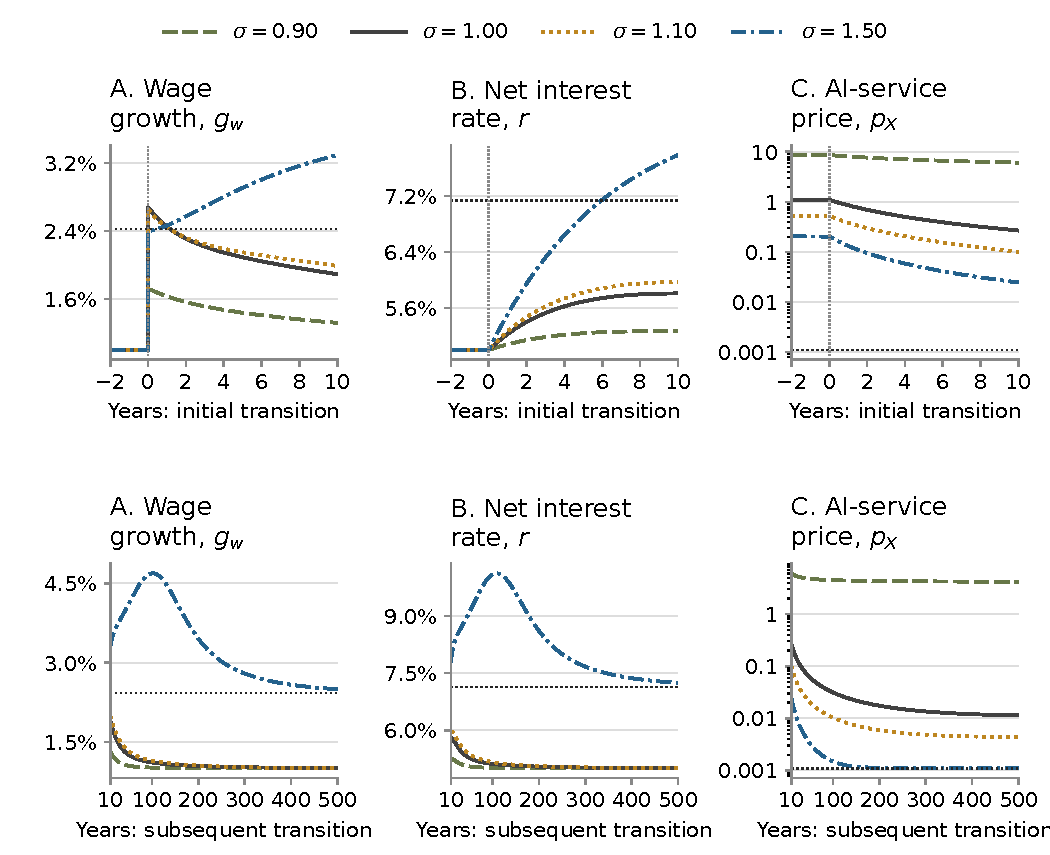
\includegraphics[width=\textwidth]{figures_rewrite/equilibrium_rsi_chi_7_5_growth_returns_windows.pdf}
 \caption{Higher research productivity ($\chi=7.5$): wage growth,
 the net interest rate, and the AI-service price. Rates are annual;
 the price is in final-good units on a logarithmic scale.
 The vertical line marks RSI activation.}
 \label{fig:rewrite-rsi-half-prices}
\end{figure}

Finally, I use Figure~\ref{fig:rewrite-rsi-half-distribution} to show labor income $wL/Y$, developer net profit $\Pi/Y$, inference expenditure $U/Y$, and research expenditure $M/Y$, all as a share of output. The top four panels show the short run and the bottom four panels show the long run. Line styles again identify the four elasticities. The omitted
gross capital income share remains $\alpha=33.0\%$.


\begin{figure}[H]
 \centering
 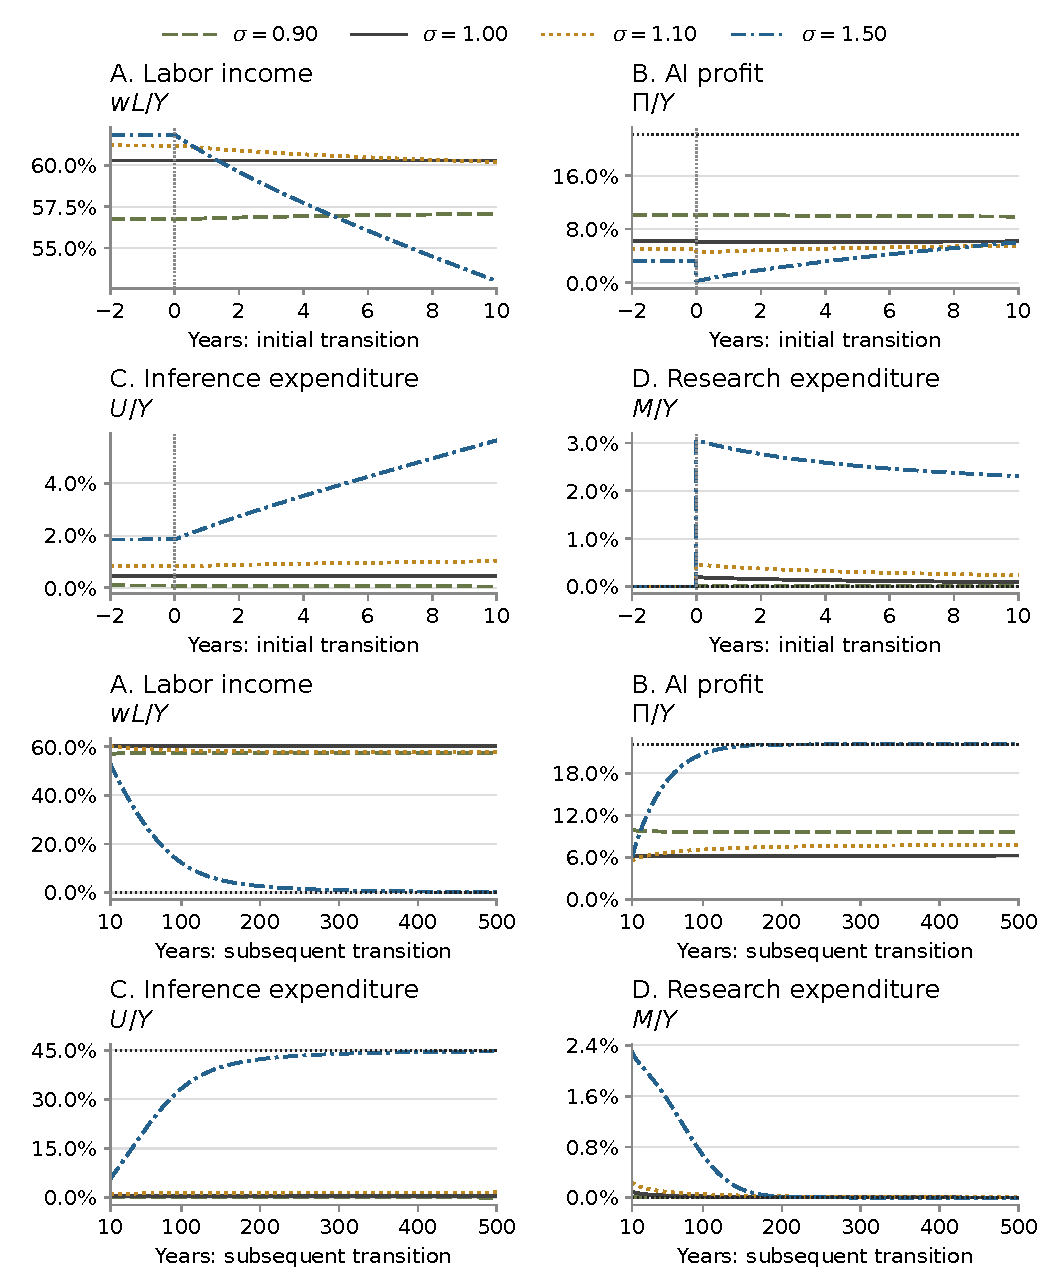
\includegraphics[width=\textwidth]{figures_rewrite/equilibrium_rsi_chi_7_5_ai_distribution_windows.pdf}
 \caption{Higher research productivity ($\chi=7.5$): labor income,
 AI net profit, inference expenditure, and research expenditure relative
 to output. The first two rows show the pre-event BGP and years 0--10;
 the last two show years 10--500. The omitted gross capital share
 remains $\alpha=0.33$. Short-run panels A and C use scales fitted to the
 initial trajectories and omit the long-run reference lines.}
 \label{fig:rewrite-rsi-half-distribution}
\end{figure}

In the short run, research spending as a share of output jumps in all four economies. The adjustment is strongest at $\sigma=1.50$: immediately after activation, research absorbs $59.4\%$ of AI revenue, compared with $35.9\%$ for inference compute. The developer's net profit therefore falls sharply. Profit subsequently recovers as research absorbs a smaller share of revenue and AI sales expand. Labor's income share also falls most strongly in this scenario, while changes are much smaller in the other three economies.

Over the longer horizon, the AI-dominated economy combines permanently faster wage growth with an even faster expansion of output per worker, so labor's income share tends to zero. Rising wages alongside a declining labor share also appear in \citet{autorkausik2026} and \citet{raymookherjee2022}. As labor's share falls, AI revenue rises relative to output. Inference compute eventually absorbs $67.0\%$ of AI revenue, while research expenditure vanishes relative to that revenue. These last proportions use AI revenue as the denominator, rather than output as in the figure.

\subsection{Lower research productivity}
\label{subsec:rewrite-rsi-research-share}

I now set $\chi=1.5$, one fifth of its value in
Section~\ref{subsec:rewrite-rsi-half-decline}. All other parameters and
initial stocks remain unchanged, including the elasticity-specific
pre-RSI capital stocks in Table~\ref{tab:rewrite-rsi-parameters}.
Consumption and research are solved again for each economy; the new
exercise changes both the initial adjustment and the timing of the
transition, but not the limiting growth rates, interest rates, and income shares.

% The generated numerical digest in rsi_chi_1_5_results.tex is retained,
% but not input here: editorial prose is organized around the three figures.
% Source: numerical_rewrite/rsi_chi_1_5/{summary,figure_manifest}.json.
I use Figure~\ref{fig:rewrite-rsi-research-accumulation} to present the growth of $Y/(AL)$, $X/(AL)$, and $K/(AL)$ in panels A--C, in percent
per year. As before, zero means growth at the rate of effective labor, $n+\gamma$. The upper row shows two pre-event years and the first ten years after RSI activation. The lower row follows the same trajectories
from year 10 to year 500. Throughout the three figures, line styles identify the same four elasticities as in Figure~\ref{fig:rewrite-rsi-half-accumulation}, and black dotted lines mark the analytical limits for $\sigma=1.50$. %Vertical scales differ between exercises.

\begin{figure}[H]
 \centering
 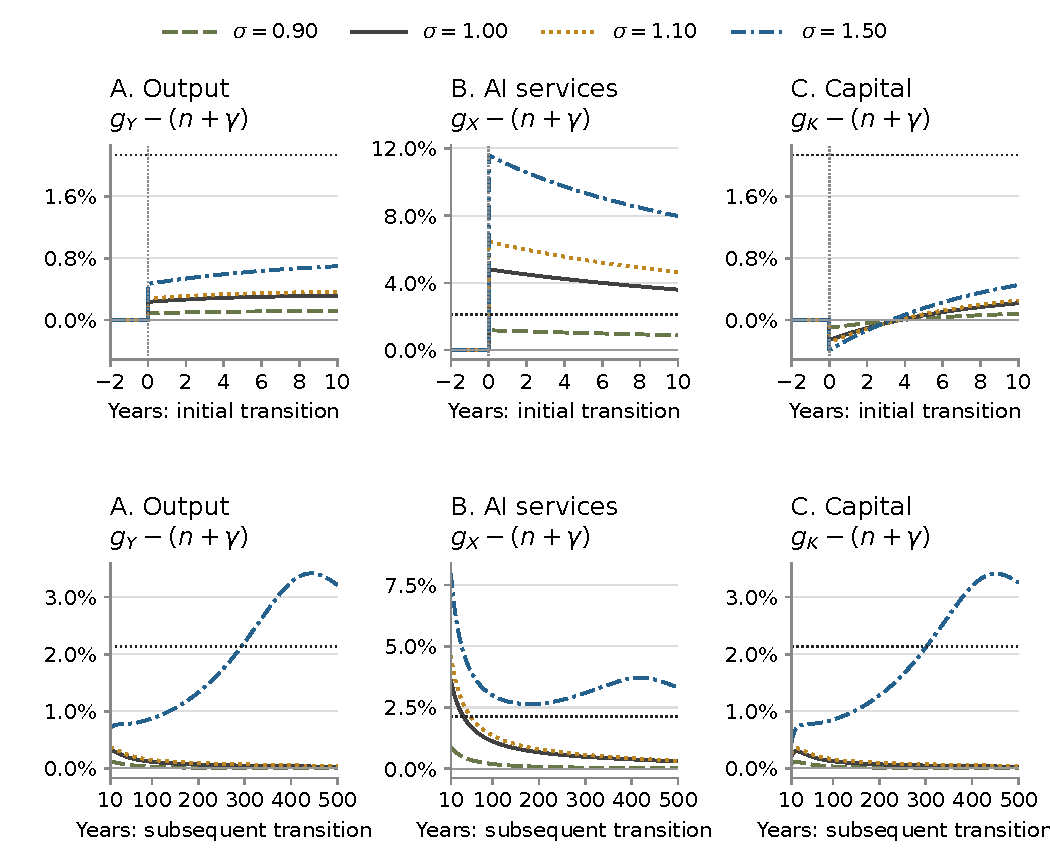
\includegraphics[width=\textwidth]{figures_rewrite/equilibrium_rsi_chi_1_5_accumulation_growth_windows.pdf}
 \caption{Lower research productivity ($\chi=1.5$): growth of output,
 AI production services, and capital per unit of effective labor.
 Rates are instantaneous annual rates. The upper row shows two pre-event
 years and years 0--10; the lower row shows years 10--500. Panels A and C
 share a scale within each row. The vertical line marks RSI activation.}
 \label{fig:rewrite-rsi-research-accumulation}
\end{figure}

The upper row shows a much smaller initial increase in growth.
Growth of $Y/(AL)$ ranges from $0.1\%$ to $0.5\%$ across the four
economies. AI services still grow faster than output, but their initial
normalized growth rate at $\sigma=1.50$ is $11.6\%$, compared with
$80.8\%$ in the preceding exercise. Lower research productivity and a
smaller research allocation produce slower efficiency improvements.
Consumption still rises at activation, and research uses resources that
could otherwise finance capital accumulation. Both adjustments are
smaller, however, so $K/(AL)$ falls less. As capital accumulation
recovers, output growth rises during the first decade even though
AI-service growth is already slowing. The four economies therefore
begin with more moderate growth and less pronounced differences.

The lower row reveals the eventual separation between regimes. At $\sigma=1.50$, output and capital growth rise for several centuries before declining. AI-service growth first slows, then rises again as capital and inference use expand. At year 500, $Y/(AL)$ still grows at $3.2\%$, above its $2.1\%$ long-run limit, showing a significantly slower transition.
A similar pattern of delayed acceleration appears in
\citet[pp.~11--12]{jones2026future}, drawing on
\citet{jonestonetti2026}. My simulations generate the transition
through private RSI investment and capital accumulation, without
modeling the progressive automation of additional tasks.
%Proposition~\ref{prop:rewrite-equilibrium-regimes} gives the same limits in both exercises of section \ref{subsec:rewrite-rsi-activation} and \ref{subsec:rewrite-rsi-half-decline}: output and capital growth rates tends to the effective labor growth rate in the three labor-bottleneck cases and remains above it at $\sigma=1.50$.

I next examine wages and prices in Figure~\ref{fig:rewrite-rsi-research-prices}. Panels A--C show annual wage growth $g_w$, the annual net interest rate $r$, and the level of $p_X$ in final-good units on a logarithmic scale. The top panels show the short run and the bottom panels the long run. Initially, wage growth rises modestly in all four economies. Unlike the preceding exercise, it continues to increase during the first years even in the labor-bottleneck cases: capital accumulation helps sustain the increase in labor's marginal product. The interest rate also rises more gradually as output outpaces capital. At $\sigma=1.50$, it reaches $5.5\%$ after ten years, compared with $7.8\%$ under higher research productivity. Meanwhile, slower efficiency improvements make the decline in $p_X$ more gradual.

In the bottom row, wage growth and the interest rate eventually turn down in all four economies. The three labor-bottleneck cases approach $1.0\%$ and $5.0\%$, respectively. At $\sigma=1.50$, the rise and
subsequent decline occur much later, and adjustment remains incomplete at year 500: the interest rate is still $8.2\%$, above its $7.1\%$
long-run value. The limiting wage-growth rate remains $2.4\%$, below output-per-worker growth of $3.1\%$. Lower research productivity therefore delays the transition without eliminating the long-run difference between these growth rates. %At year 500, the AI-service price in this case is already close to its positive limit, even though growth and interest rates are still adjusting.

\begin{figure}[H]
 \centering
 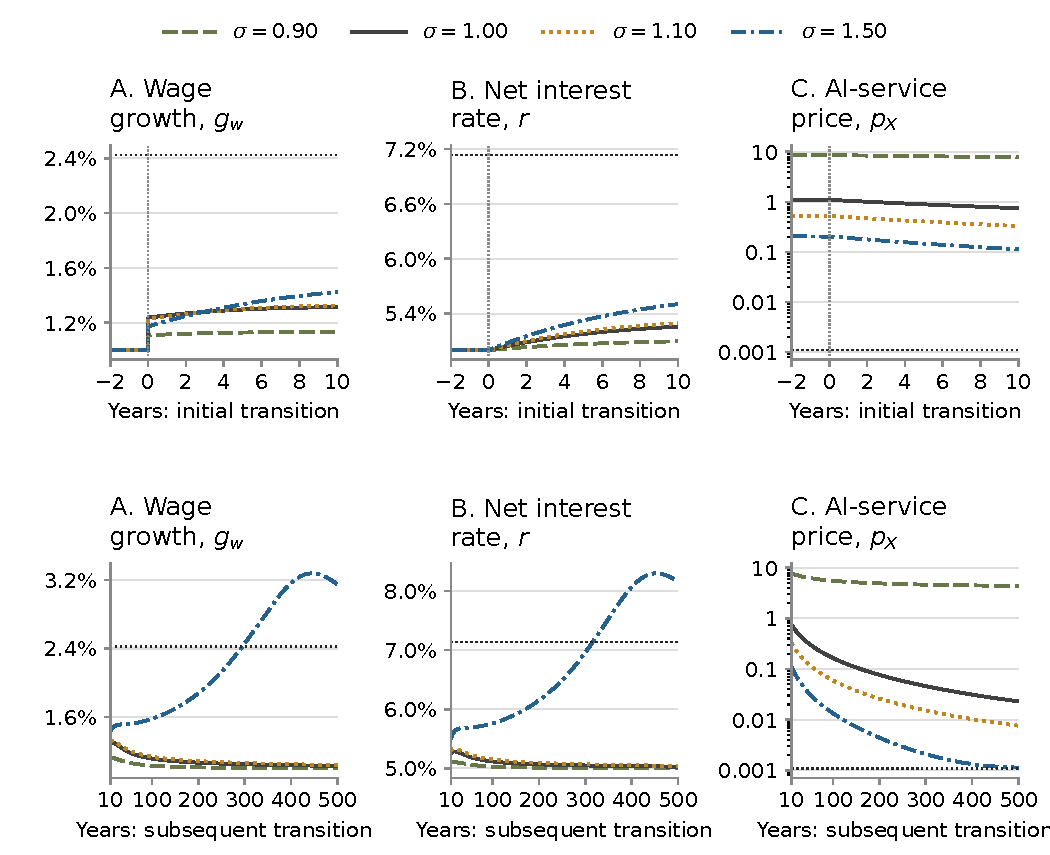
\includegraphics[width=\textwidth]{figures_rewrite/equilibrium_rsi_chi_1_5_growth_returns_windows.pdf}
 \caption{Lower research productivity ($\chi=1.5$): wage growth,
 the net interest rate, and the AI-service price. Rates are annual;
 the price is in final-good units on a logarithmic scale.
 The vertical line marks RSI activation.}
 \label{fig:rewrite-rsi-research-prices}
\end{figure}

I complete the comparison with Figure~\ref{fig:rewrite-rsi-research-distribution}. Panels A--D report
$wL/Y$, $\Pi/Y$, $U/Y$, and $M/Y$, all as percentages of output. The upper two rows cover the initial transition and the lower two cover years 10--500, with the same scenario lines. The omitted gross capital share remains $33.0\%$.

\begin{figure}[H]
 \centering
 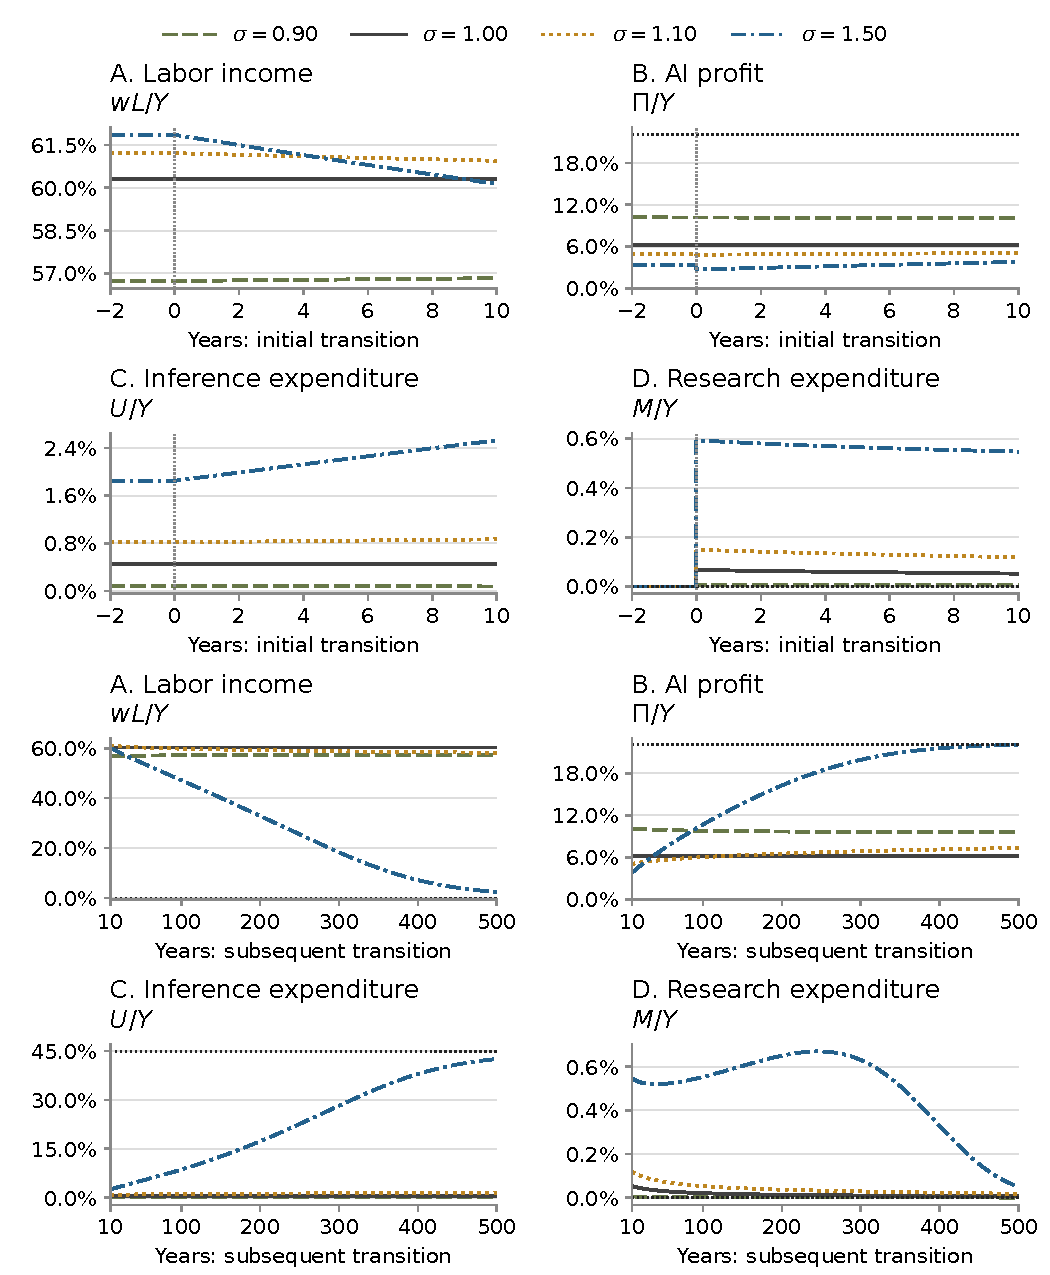
\includegraphics[width=\textwidth]{figures_rewrite/equilibrium_rsi_chi_1_5_ai_distribution_windows.pdf}
 \caption{Lower research productivity ($\chi=1.5$): labor income,
 AI net profit, inference expenditure, and research expenditure relative
 to output. The first two rows show the pre-event BGP and years 0--10;
 the last two show years 10--500. The omitted gross capital share
 remains $\alpha=0.33$. Short-run panels A and C use scales fitted to the
 initial trajectories and omit the long-run reference lines.}
 \label{fig:rewrite-rsi-research-distribution}
\end{figure}

In the short run, research absorbs a smaller share of output, leaving more of AI revenue as net profit. At $\sigma=1.50$, initial research expenditure is $0.6\%$ of output rather than $3.1\%$, and net profit is $2.7\%$ rather than $0.2\%$. Research spending reduces net profit at activation, but less sharply than in the preceding exercise. Inference expenditure and labor's income share change little in the labor-bottleneck cases. In the AI-dominated case, inference's share increases and labor's share declines, but both movements are initially gradual, consistent with the smaller output--wage growth gap.

The longer horizon shows the same eventual redistribution as in Figure~\ref{fig:rewrite-rsi-half-distribution}: labor's share tends to zero at $\sigma=1.50$, while inference expenditure and developer profit approach the same positive shares of output. Research expenditure relative to output first declines, then rises again before falling toward zero. Expanding AI sales provide an incentive for further research, while proximity to the upper bound eventually limits the efficiency gains it can deliver. %The research condition~\eqref{eq:rewrite-research-foc} balances these changing benefits against the cost of compute; $\chi$ alone does not determine the research path.
The other three economies retain a positive labor share. Lower research productivity changes the adjustment and delays the divergence between regimes without changing their limiting growth rates and income shares.

\subsection{From competitive provision to monopoly with RSI}
\label{subsec:rewrite-competitive-transition}

I now examine a different experiment: granting exclusive rights over AI
technology in an economy that initially supplies AI services competitively.
This allows me to compare the initial restriction in AI use with the
subsequent efficiency gains financed by monopoly rents. Unlike the
preceding exercises, RSI is available before date zero, with the same
positive $\chi$ as after the change. Research is nevertheless zero under
the free-access arrangement in Section~\ref{sec:rewrite-competition},
because improvements cannot be privately appropriated.

I retain the parameters in Table~\ref{tab:rewrite-rsi-parameters}, including
both research productivities and all four elasticities, but choose $K_0$
to place each economy on its competitive BGP at the same $B_0$. Before
the change, $p_X=1/B_0$, $r=\rho+\gamma$, and $K_0/Y_0=3.3$.
Table~\ref{tab:rewrite-competitive-transition} reports the new capital
stocks. In every case, continued competition would preserve the
labor-bottleneck BGP, with output per worker, consumption per person,
and wages growing at $\gamma$.

At date zero, an unexpected permanent exclusive right covers both the
existing AI technology and its subsequent improvements. In particular,
competitive suppliers can no longer use the old technology. The economy
then follows the monopoly equilibrium, inheriting $K_0$ and $B_0$ but
choosing consumption and research anew. This experiment changes research
incentives and pricing, not the RSI technology. It abstracts from the
cost of enforcing exclusivity and is not an optimal policy exercise.

\begin{table}[H]
 \centering
 \caption{Competitive initial capital and the impact of exclusive AI rights}
 \label{tab:rewrite-competitive-transition}
 \small\setstretch{1.0}
 \begin{tabular}{cccc}
 \toprule
 $\sigma$ & $K_0$ & Change in output & Change in wage\\
 \midrule
 0.9 & 6.235 & $-32.4\%$ & $-36.6\%$\\
 1.0 & 6.278 & $-17.6\%$ & $-17.6\%$\\
 1.1 & 6.324 & $-13.7\%$ & $-11.9\%$\\
 1.5 & 6.535 & $-10.4\%$ & $-5.4\%$\\
 \bottomrule
 \end{tabular}
 \par\vspace{4pt}
 \parbox{0.95\textwidth}{\footnotesize\emph{Notes:} The capital stocks are
 derived from the competitive BGP, not selected independently. All other
 parameters and initial stocks are in Table~\ref{tab:rewrite-rsi-parameters}.
 Changes compare levels immediately after and before the grant. They are
 identical for both values of $\chi$, since $K$ and $B$ cannot jump.
 The ratio $K_0/Y_0=3.3$ applies before the grant, not after output falls.}
\end{table}

I first consider $\chi=7.5$ in
Figure~\ref{fig:rewrite-competitive-high-levels}. Panels A--C show output
per worker, wages, and consumption per person, each relative to continued
competition from the same initial stocks. The line styles identify the
four elasticities as in the preceding figures. The upper row includes
two pre-event years and years 0--10; the middle row shows years 10--100;
the lower row shows years 10--500. The competitive benchmark is
$100.0\%$ in the upper row and one in the logarithmic lower rows.
The intermediate window makes recoveries visible that would be
compressed in the 500-year view.

The initial markup reduces AI use, output, and wages before efficiency
can improve. At $\sigma=1.5$, output and wages fall by $10.4\%$ and
$5.4\%$, respectively. Research subsequently raises efficiency, and
output first regains its competitive counterpart around year 3.8;
wages do so around year 4.6. Consumption instead rises by $8.2\%$ at
the grant, even as output falls. The household chooses less capital
accumulation, while reduced inference use releases some resources.
The consumption response therefore need not have the same sign as the
output response.

\begin{figure}[H]
 \centering
 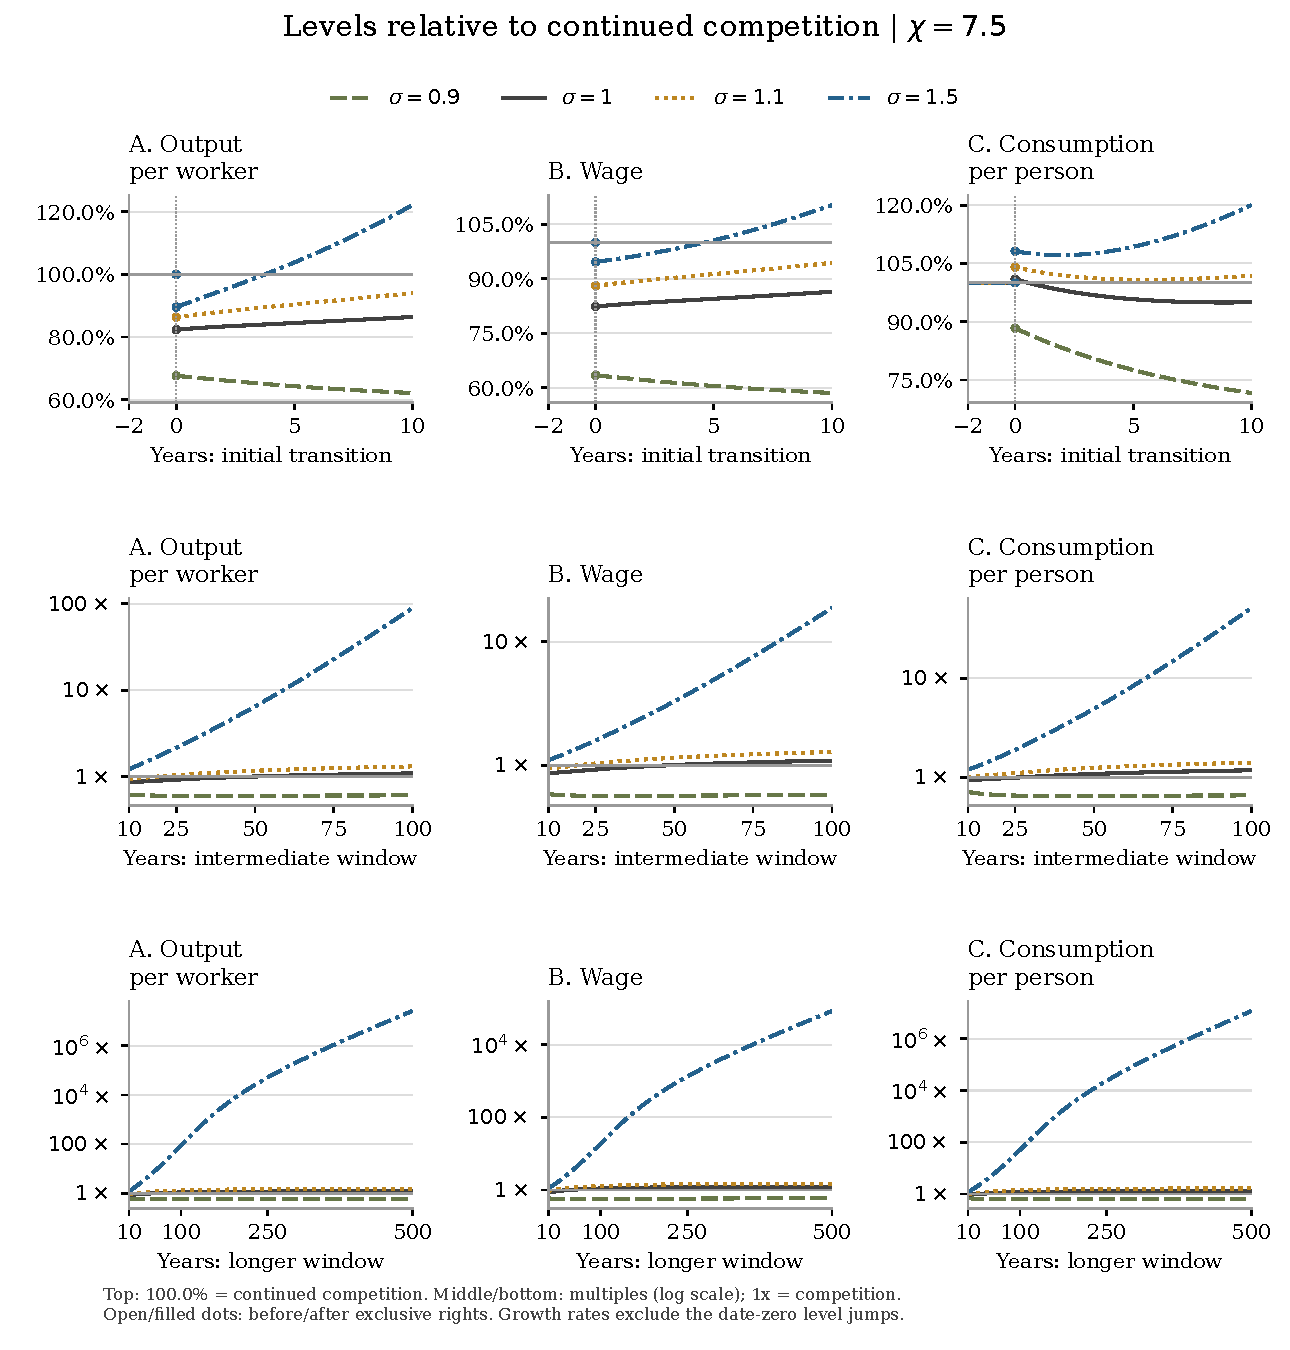
\includegraphics[width=\textwidth]{figures_rewrite/competitive_to_monopoly/competitive_to_monopoly_chi_7_5_levels.pdf}
 \caption{From competition to monopoly with RSI, $\chi=7.5$: levels
 relative to continued competition. The rows cover years $-2$--10,
 10--100, and 10--500. The upper row uses percentages; the middle and
 lower rows use multiples on logarithmic scales. The horizontal
 benchmark is $100.0\%$ or $1\times$. Open and filled dots mark levels
 before and after the grant. Vertical scales differ across windows
 and between the two research-productivity exercises.}
 \label{fig:rewrite-competitive-high-levels}
\end{figure}

The middle row shows that recovery is not confined to the AI-dominated
case. Output catches up around year 18.2 at $\sigma=1.1$ and year 46.9
at $\sigma=1$. These economies obtain level gains even though their
long-run output-per-worker and wage growth return to $\gamma$.
By contrast, the lower row shows an expanding gap at $\sigma=1.5$:
the monopoly economy approaches the AI-dominated regime, while the
competitive counterfactual remains labor-bottlenecked. At $\sigma=0.9$,
neither output nor wages recover within 500 years. Higher AI efficiency
does not necessarily compensate for restricted access to AI services.

I next lower research productivity to $\chi=1.5$ in
Figure~\ref{fig:rewrite-competitive-low-levels}, using the same stocks,
comparison, and time windows. The initial output and wage losses are
unchanged, but research absorbs less output: at $\sigma=1.5$, its initial
share is $0.6\%$ rather than $3.3\%$. Consumption initially rises by
$3.7\%$ rather than $8.2\%$. Lower research productivity thus changes
the initial allocation as well as the speed of subsequent improvement.
Output and wages at $\sigma=1.5$ remain below the competitive benchmark
throughout the first decade, recovering only around years 24.0 and
26.0. Output at $\sigma=1.1$ recovers around year 87.3, whereas at
$\sigma=1$ recovery falls outside the intermediate window, around
year 212.3.

\begin{figure}[H]
 \centering
 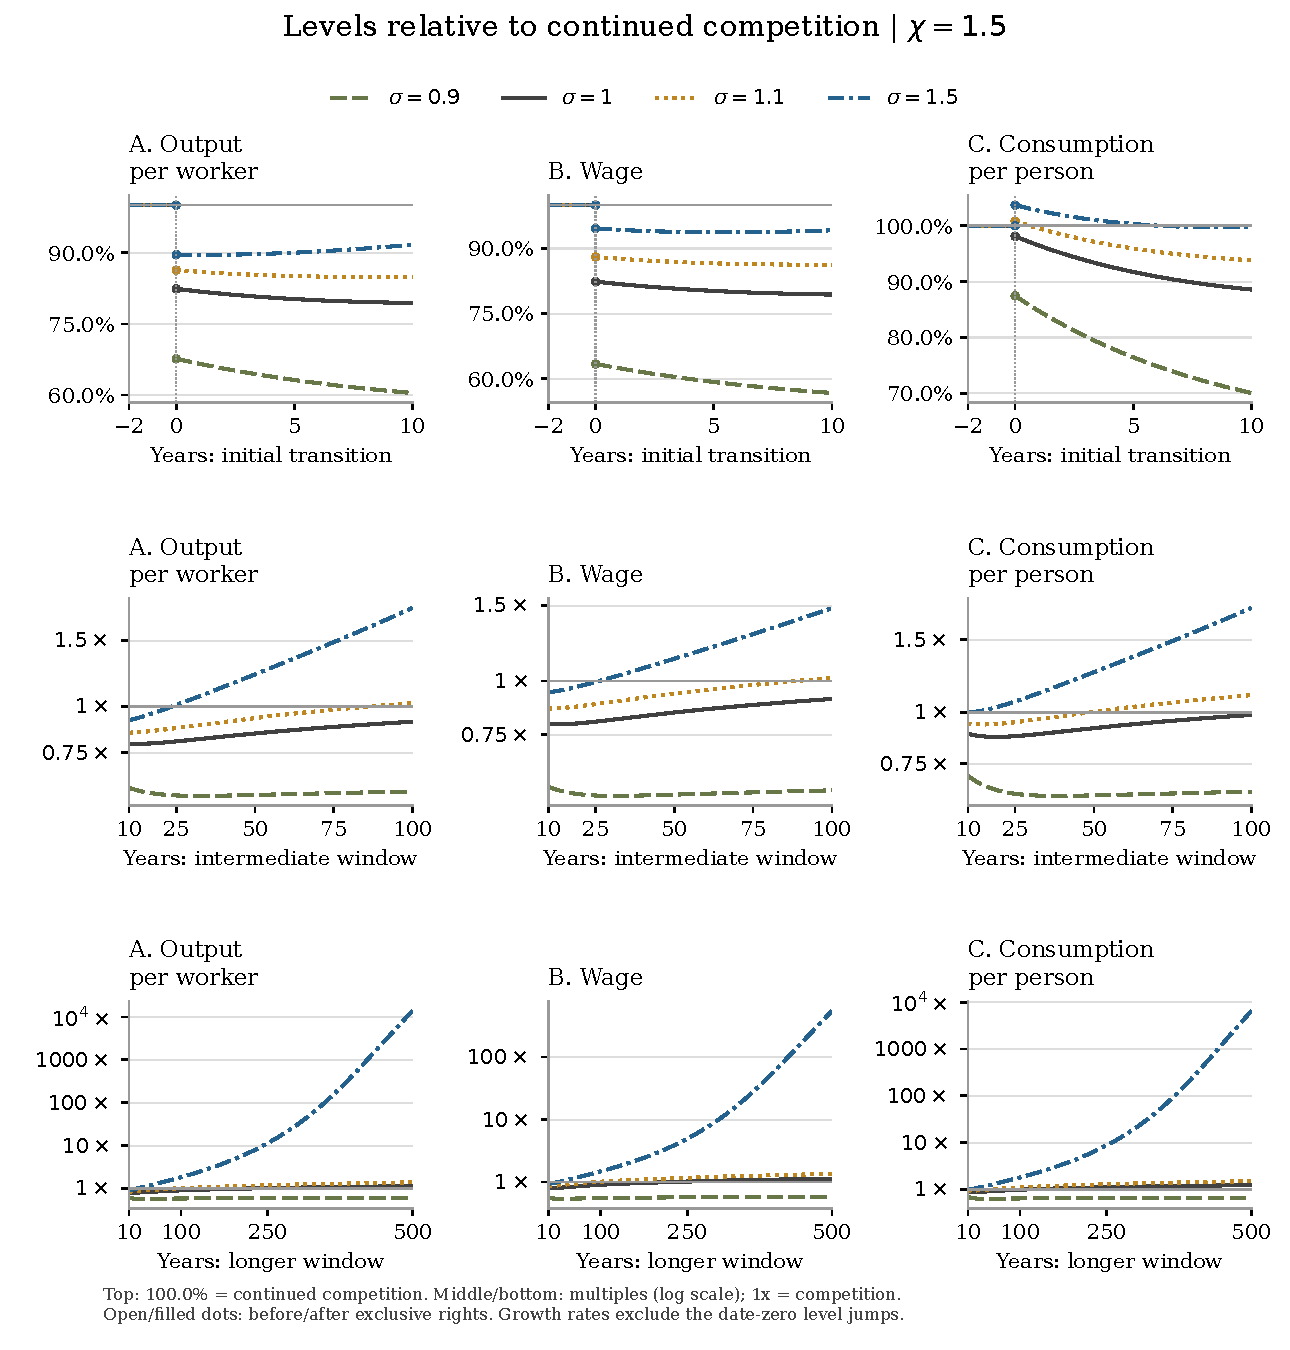
\includegraphics[width=\textwidth]{figures_rewrite/competitive_to_monopoly/competitive_to_monopoly_chi_1_5_levels.pdf}
 \caption{From competition to monopoly with RSI, $\chi=1.5$: output
 per worker, wages, and consumption per person relative to continued
 competition. Windows, normalizations, and line styles match
 Figure~\ref{fig:rewrite-competitive-high-levels}; vertical scales are
 fitted to this exercise. The middle row reveals recoveries outside
 the first decade, while the lower row retains the longer transition.}
 \label{fig:rewrite-competitive-low-levels}
\end{figure}

Research productivity changes these recoveries, not the monopoly limits
in Proposition~\ref{prop:rewrite-equilibrium-regimes}. At $\sigma=1.5$,
limiting output-per-worker growth, wage growth, and the interest rate
are $3.1\%$, $2.4\%$, and $7.1\%$ under either $\chi$. The lower rows
show the separation from continued competition, not completed
convergence: the interest rate at year 500 is still $7.2\%$ with high
research productivity and $8.2\%$ with low research productivity.
Appendix~\ref{app:rewrite-competitive-transition} reports growth,
prices, income shares, and compute expenditure for all eight paths.

I interpret these simulations as an institutional counterfactual, not
as a calibrated prediction of granting AI exclusivity. In particular,
the impact price at $\sigma=0.9$ is about 131 times its competitive
level, a large distortion implied by the inherited parameters.
The recovery dates compare contemporaneous levels, not cumulative
gains or household welfare. Evaluating the policy would require the
entire consumption path, not just the date at which output or wages
overtake continued competition.

% Section 6.4 is silenced at the author's request; its source remains intact.
% Uncomment the following input to restore it.
%\input{sections_rewrite/11_rsi_limitations}
\section{Conclusion}
\label{sec:rewrite-conclusion}

This paper endogenizes investment in AI research, which in turn affects the pace of economic growth. Even under RSI, computing requires resources that compete with consumption and accumulation of physical capital. Algorithms and model weights, by contrast, are non-rival: using them does not deplete them. Following \citet{romer1990}, I use monopoly rents to make research investment profitable. In practice, firms compete to develop algorithms and train models. However, as
\citet{korinekvipra2025} explain, access to better AI can improve the advantage of a leading developer, so an eventual monopoly does not seem to be far-fetched. The prospect of future monopoly rents can help explain intense competition among firms.  %Allowing entry, competing developers, and knowledge diffusion would help determine how competition changes investment, prices, income distribution, and the pace of economic growth.

With an upper bound on AI efficiency, permanently faster wage growth requires sufficient substitution between AI and labor and sufficiently high attainable efficiency. In this AI-dominated regime, output and AI revenue per worker grow faster than wages, so labor's income share vanishes even as wages rise. AI-dominated growth can permanently increase the return on capital, raising questions about
wealth concentration not examined here \citep{bergbuffiezanna2018,mollrachelrestrepo2022}. When labor remains a production bottleneck, the growth rates of output per worker and wages instead return to the exogenous rate of labor-augmenting technological progress. The upper bound on AI efficiency matters for these growth and distributional outcomes: without it, the unit-elasticity case can sustain both growth rates above this exogenous rate while preserving a positive labor share.

RSI is not sufficient for permanently faster output-per-worker growth, nor does such growth require continuing improvements in AI efficiency. AI efficiency can improve even when labor remains a production bottleneck. Under complementarity, output-per-worker growth cannot permanently exceed the rate of labor-augmenting technological progress, even without an upper bound on AI efficiency. With
sufficient substitution and sufficiently high attainable AI efficiency,
capital accumulation and expanding inference compute sustain permanently
faster growth in both output per worker and wages, even as AI efficiency
converges to its upper bound.

The comparison with competition separates the efficiency needed to
sustain AI-dominated growth from the incentives to reach it. Under free
access to AI models and their improvements, competitive suppliers do not
finance RSI. Nevertheless, sufficiently high initial efficiency sustains
AI-dominated growth without monopoly or further research. From a lower
initial efficiency, monopoly rents can finance improvements that allow
an escape from the labor bottleneck. But markups restrict AI use and
raise the efficiency required relative to marginal-cost pricing.
Competition can therefore sustain AI-dominated growth where monopoly
produces more efficient AI but leaves the economy labor-bottlenecked.
Even when both economies are AI-dominated, monopoly delivers faster
growth only if its efficiency gains outweigh this restriction.
Neither market structure nor efficiency alone determines which economy
grows faster. These comparisons do not rank welfare.

Removing monopoly rents after innovation
can undermine the credibility of the incentives offered beforehand.
Patent buyouts could instead reward the developer while opening access
to existing AI technology \citep{kremer1998}. An extension could study
how to value and finance such buyouts while preserving incentives
for further RSI.

Simulations show that early output-per-worker growth can look similar across economies approaching different long-run regimes. The question remains whether human labor will be essential enough for wages to keep pace with output per worker.



% END REVISED CONCLUSION

%The bottleneck mechanism has antecedents in \citet{aghionjonesjones2019}, and rising wages alongside a declining labor share are not themselves new predictions \citep{jones2026future}. In the equilibria I characterize with private investment in RSI, substitutability alone does not suffice: attainable AI efficiency must alsoexceed a threshold that makes capital accumulation sufficiently productive. Above it, higher attainable efficiency raises long-run growth and the interest rate. The wage-growth premium over the exogenous rate equals the output-per-worker growth premium divided by the substitution elasticity, which measures how much of the growth acceleration reaches wages.

%Complementarity prevents output per worker from growing permanently faster than labor-augmenting technological progress. At unit elasticity, however, continued AI improvement can sustain faster output and wage growth with a positive labor share. With substitution and sufficiently strong research returns, the developer's discounted net profit is unbounded even on a fixed finite horizon. This is a failure of the optimization problem, not a proof that an equilibrium reaches a finite-time singularity. Equilibrium existence without an upper bound remains unresolved for the remaining substitution cases.

%The simulations show that moderate early growth can precede either the AI-dominted regime or the labor-bottleneck regime. long-run regime. Research productivity changes both the initial reallocation of resources and the timing of the divergence, not just the speed along a fixed path. It does not change the limiting outcomes in the finite-upper-bound regimes studied here. These are illustrative scenarios, not joint empirical fits to AI revenues, research expenditure, and prices. Limited information on compute allocation also constrains calibration \citep{korinekmckelvey2026}. I therefore place more weight on the conditional long-run results than on the dates of takeoff.

%The abrupt initial adjustment depends on an unanticipated activation of RSI, reversible capital, and compute supplied without installation delays. Gradual adoption and an explicit compute sector with investment frictions would test how much of this adjustment remains when capacity takes time to expand. The model of \citet{erdiletal2025gate} provides a framework for such frictions. Introducing human research tasks and allowing attainable efficiency to evolve would also test the technological assumptions, drawing on the research networks and bottlenecks in \citet{davidsonetal2026}.

%Permanent monopoly restricts the relationship between AI revenue, prices, and research incentives. Together with the production technology, it can imply a substantial AI revenue share even under complementarity; a profitable AI industry need not signal permanently faster growth. Revenue also differs from net profit after inference and research costs. I retain the AI production weight as an illustrative parameter, not an estimate of the industry's size. The concentration and competition mechanisms discussed by \citet{korinekvipra2025} motivate an extension with entry and competing developers to examine how market structure affects private RSI investment.

%The aggregate labor input excludes differences across occupations and the creation of new tasks in which workers retain a comparative advantage. Incorporating the displacement and reinstatement mechanisms of \citet{acemoglurestrepo2019} would allow labor's role to change through task creation and automation, rather than only through relative input use. The present model cannot determine which workers gain or lose during the transition. Nor should its aggregate substitution threshold be interpreted as a restriction on models with different task structures.

%Finally, a declining labor share does not by itself determine household inequality or workers' economic power. The representative household owns capital and the AI developer, so I do not distinguish workers who rely on wages from households that receive most of the profits. As \citet{jones2026future} emphasizes, asset ownership and redistribution matter for who shares in AI-driven prosperity. In \citet{mollrachelrestrepo2022}, automation increases wealth concentration by raising returns to wealth. Heterogeneous ownership and a fiscal sector would allow me to study how capital income and transfers modify the distribution of gains described here through wages and factor shares.

%\enlargethispage{\baselineskip}
%If there is no bound on AI capabilities, the question becomes whether human labor will remain sufficiently essential for wages to keep pace with the rest of the economy.


\appendix
\Needspace{12\baselineskip}
\section{Proofs}
\label{app:rewrite-proofs}

\Needspace{7\baselineskip}
\begin{lemma}[Static AI-service choice]
\label{lem:rewrite-monopoly-choice}
For $K,A,L,B>0$, $0<\alpha<1$, $\sigma>0$, and strictly positive CES weights
that sum to one, problem~\eqref{eq:rewrite-service-choice} has a unique,
strictly positive global maximizer. It is characterized by
condition~\eqref{eq:rewrite-monopoly-foc} and depends smoothly on the positive
variables $K,A,L,B$, for each fixed $\sigma$.
\end{lemma}

\begin{proof}[Proof of Lemma~\ref{lem:rewrite-monopoly-choice}]
Fix \(K,A,L,B>0\) and let \(R(X)=p_X(X)X\).
The demand elasticity in \eqref{eq:rewrite-inverse-demand-elasticity} and the
CES-share derivative imply
\[
 R'(X)=p_X(X)(1-e_X),\qquad
 \frac{\dd s_X}{\dd\ln X}=\left(1-\frac1\sigma\right)s_X(1-s_X).
\]
Wherever marginal revenue is positive, direct differentiation gives
\begin{equation}
 -\frac{XR''(X)}{p_X(X)}
 =e_X(1-e_X)+\left(\alpha-\frac1\sigma\right)
 \left(1-\frac1\sigma\right)s_X(1-s_X).
 \label{eq:rewrite-monopoly-proof-curvature}
\end{equation}
If \((\alpha-1/\sigma)(1-1/\sigma)\geq0\), the right-hand side is positive.
If this product is negative, the parameter restrictions imply
\(0<\alpha<1/\sigma<1\), and
\[
 \begin{aligned}
 -\frac{XR''(X)}{p_X(X)}
 ={}&\frac1\sigma\left(1-\frac1\sigma\right)(1-s_X)^2\\
 &+\left[\frac1{\sigma^2}+2\alpha-\frac{3\alpha}{\sigma}\right]s_X(1-s_X)
 +\alpha(1-\alpha)s_X^2.
 \end{aligned}
\]
The middle coefficient is positive because
\[
 \frac1{\sigma^2}+2\alpha-\frac{3\alpha}{\sigma}
 =\left(\frac1\sigma-\alpha\right)^2
 +\alpha\left(2-\frac1\sigma-\alpha\right)>0.
\]
Thus marginal revenue decreases strictly whenever it is positive.

As \(X\downarrow0\), revenue is proportional to \(X^{1-1/\sigma}\) when
\(\sigma>1\), to \(X^{(1-\alpha)\omega_X}\) when \(\sigma=1\), and to
\(X^{1-\alpha}\) when \(\sigma<1\). Every exponent lies between zero and
one, so \(R'(X)\to\infty\). As \(X\to\infty\), marginal revenue converges to
zero from above if \(\sigma\geq1\); if \(\sigma<1\), it eventually
becomes negative. Hence \(R'(X)=1/B\) has exactly one solution. Operating profit
increases before this solution and decreases after it. The linear cost \(X/B\)
dominates revenue as \(X\to\infty\), so this solution is the unique global
maximum. Equation \eqref{eq:rewrite-monopoly-proof-curvature} also proves the
strict second-order condition:
\begin{equation}
 e_X(1-e_X)
 +\left(\alpha-\frac1\sigma\right)\left(1-\frac1\sigma\right)s_X(1-s_X)>0.
 \label{eq:rewrite-monopoly-soc}
\end{equation}
At the unique solution of $R'(X)=1/B$, $R''(X)<0$.
The implicit-function theorem therefore makes the maximizing service choice
smooth in $K,A,L,B$.
\end{proof}

\begin{lemma}[Optimal research expenditure]
\label{lem:rewrite-developer-verification}
Consider a feasible research trajectory $\{B_t,M_t\}_{t\geq0}$
for problem~\eqref{eq:rewrite-developer-reduced}, starting from
$B_0$ and satisfying the RSI technology
\eqref{eq:rewrite-capability-law}. Suppose $M_t>0$ and the
present value of net profit is finite. Suppose there exists
a continuously differentiable shadow-price trajectory
$\{q_t\}_{t\geq0}$ satisfying the research condition
\eqref{eq:rewrite-research-foc}, the costate equation
\eqref{eq:rewrite-costate}, and the transversality condition
\eqref{eq:rewrite-developer-tvc}.

Suppose $0<B_0<\overline B<\infty$ and, for every $t\geq0$
and every $b\in[B_0,\overline B)$,
\begin{equation}
 \begin{aligned}
 \pi_t(b)-\pi_t(B_t)
 &+\frac{1-\eta}{\eta}M_t
 \left[
 \left(\frac{b}{B_t}\right)^{\eta/(1-\eta)}-1
 \right]\\
 &\leq
 \frac{\overline B-B_t}{B_t}(U_t+M_t)
 \log\!\left(
 \frac{\overline B-B_t}{\overline B-b}
 \right),
 \end{aligned}
 \label{eq:rewrite-hamiltonian-support}
\end{equation}
where $\pi_t(b)$ is operating profit as defined in
equation~\eqref{eq:rewrite-service-choice}.
Then $\{M_t\}_{t\geq0}$ solves the developer's
problem~\eqref{eq:rewrite-developer-reduced}:
no other feasible research trajectory starting from
the same $B_0$ yields a higher present value of net profit.
\end{lemma}

\begin{proof}[Proof of Lemma~\ref{lem:rewrite-developer-verification}]
For the proof, define the transformed AI-efficiency state, or research depth, by
\begin{equation}
 R_B(B)=-\overline B\log\left(1-\frac{B}{\overline B}\right),
 \qquad
 B(R_B)=\overline B\left(1-e^{-R_B/\overline B}\right).
 \label{eq:rewrite-research-depth}
\end{equation}
It maps $B\in[B_0,\overline B)$ into
$R_B\in[R_{B,0},\infty)$, where $R_{B,t}=R_B(B_t)$ and
$R_{B,0}=R_B(B_0)$. Since $R_B'(B)=1/\psi(B)$, this transformation removes
the factor $\psi(B)$ from the RSI technology~\eqref{eq:rewrite-capability-law}:
\begin{equation}
 \dot R_B=\chi[B(R_B)M]^\eta.
 \label{eq:rewrite-research-depth-law}
\end{equation}
The corresponding current-value shadow price is $q_{R,t}=q_t\psi(B_t)$,
which is positive by the research condition~\eqref{eq:rewrite-research-foc}.
At each date $t$, hold $q_{R,t}$ at its value along the candidate trajectory
and define the maximized Hamiltonian for an alternative state $\widetilde R_B$:
\[
 \widehat{\mathcal H}_t(\widetilde R_B)
 \equiv\max_{\widetilde M\geq0}
 \left\{\pi_t(B(\widetilde R_B))-\widetilde M
 +q_{R,t}\chi[B(\widetilde R_B)\widetilde M]^\eta\right\}.
\]
Because $0<\eta<1$, the expression being maximized is strictly concave in
research expenditure. Using the candidate's research
condition~\eqref{eq:rewrite-research-foc}, the maximizing expenditure at
$\widetilde R_B$ is
\[
 M_t\left[\frac{B(\widetilde R_B)}{B_t}\right]^{\eta/(1-\eta)},
\]
where $M_t$ is the candidate's research expenditure. Substitution gives
\begin{equation}
 \widehat{\mathcal H}_t(\widetilde R_B)
 =\pi_t(B(\widetilde R_B))+
 \frac{1-\eta}{\eta}M_t
 \left[\frac{B(\widetilde R_B)}{B_t}\right]^{\eta/(1-\eta)}.
 \label{eq:rewrite-maximized-depth-hamiltonian}
\end{equation}
Differentiating the maximized Hamiltonian with respect to its state argument
and using the envelope condition~\eqref{eq:rewrite-profit-envelope} gives
\begin{equation}
 \widehat{\mathcal H}'_t(R_{B,t})
 =\frac{\psi(B_t)}{B_t}(U_t+M_t).
 \label{eq:rewrite-depth-hamiltonian-slope}
\end{equation}
Because
\[
 R_B(b)-R_{B,t}
 =\overline B\log\!\left(\frac{\overline B-B_t}{\overline B-b}\right),
\]
condition~\eqref{eq:rewrite-hamiltonian-support} is equivalent to the
following inequality for every $\widetilde R_B\geq R_{B,0}$:
\[
 \widehat{\mathcal H}_t(\widetilde R_B)
 \leq\widehat{\mathcal H}_t(R_{B,t})
 +\widehat{\mathcal H}'_t(R_{B,t})
 (\widetilde R_B-R_{B,t}).
\]

Let $D_t=\exp(-\int_0^t r_s\dd s)$ be the discount factor and
$\mu_t=D_tq_{R,t}$ the present-value shadow price of research depth.
The research condition~\eqref{eq:rewrite-research-foc} and the RSI
technology~\eqref{eq:rewrite-capability-law} imply $q_t\eta\dot B_t=M_t$.
Differentiating $q_{R,t}=q_t\psi(B_t)$ and using the costate
equation~\eqref{eq:rewrite-costate} therefore gives
\[
 \dot q_{R,t}=r_tq_{R,t}-\frac{\psi(B_t)}{B_t}(U_t+M_t),
 \qquad
 \dot\mu_t=-D_t\widehat{\mathcal H}'_t(R_{B,t}).
\]

Consider any feasible alternative $\{\widetilde B_t,\widetilde M_t\}_{t\geq0}$
starting from the same $B_0$, and write $\widetilde R_{B,t}=R_B(\widetilde B_t)$.
Here feasible expenditure is nonnegative and integrable on every finite
interval, with a locally absolutely continuous state satisfying the RSI
technology almost everywhere.
Let
\[
 J_T=\int_0^T D_t[\pi_t(B_t)-M_t]\dd t
\]
denote discounted net profit through date $T$ under the candidate, and define
$\widetilde J_T$ analogously for the alternative.
At each date, the alternative's Hamiltonian cannot exceed
$\widehat{\mathcal H}_t(\widetilde R_{B,t})$, whereas the candidate attains
$\widehat{\mathcal H}_t(R_{B,t})$. Applying
condition~\eqref{eq:rewrite-hamiltonian-support} and the transformed costate
equation yields, for almost every $t$,
\[
 \begin{aligned}
 &D_t\left[
 \pi_t(\widetilde B_t)-\widetilde M_t
 -\pi_t(B_t)+M_t
 \right]\\
 &\quad\leq D_t\widehat{\mathcal H}'_t(R_{B,t})
 (\widetilde R_{B,t}-R_{B,t})
 -\mu_t(\dot{\widetilde R}_{B,t}-\dot R_{B,t})\\
 &\quad=-\frac{\mathrm d}{\mathrm dt}
 \left[\mu_t(\widetilde R_{B,t}-R_{B,t})\right].
 \end{aligned}
\]
Integrating from zero to $T$ and using the common initial
state gives
\[
 \widetilde J_T-J_T
 \leq-\mu_T(\widetilde R_{B,T}-R_{B,T})
 \leq\mu_TR_{B,T},
\]
where the second inequality uses $\mu_T>0$ and $\widetilde R_{B,T}\geq0$.
Since
\[
 \psi(B_t)R_{B,t}
 =-(\overline B-B_t)\log\left(1-\frac{B_t}{\overline B}\right)
 \leq B_t,
\]
the developer's transversality condition~\eqref{eq:rewrite-developer-tvc} gives
\[
 0\leq\mu_TR_{B,T}
 =D_Tq_T\psi(B_T)R_{B,T}
 \leq D_Tq_TB_T\longrightarrow0.
\]
The candidate's present value is finite by assumption. Hence
\[
 \limsup_{T\to\infty}\widetilde J_T
 \leq\lim_{T\to\infty}J_T<\infty,
\]
so no feasible alternative yields a higher present value of net profit.
The argument requires a global upper tangent at the candidate state at each
date, not concavity at every counterfactual state.
\end{proof}

\Needspace{8\baselineskip}
\begin{lemma}[Sufficient conditions for Hamiltonian concavity]
\label{lem:rewrite-hamiltonian-concavity}
Consider the maximized Hamiltonian in
equation~\eqref{eq:rewrite-maximized-depth-hamiltonian} for a feasible
trajectory satisfying the research condition~\eqref{eq:rewrite-research-foc},
with $M_t>0$ and $0<B_0<\overline B<\infty$.
Let $X_t^*(b)$ denote the optimal AI-service choice in
problem~\eqref{eq:rewrite-service-choice} at efficiency $b$, and let
$\varepsilon_{B,t}(b)=\partial\ln X_t^*(b)/\partial\ln b$
denote its elasticity with respect to AI efficiency.
Suppose that, for every $t\geq0$ and $b\in[B_0,\overline B)$,
\begin{equation}
 \psi(b)[\varepsilon_{B,t}(b)-2]\leq\frac{b}{\overline B},
 \label{eq:rewrite-capped-concavity-gate}
\end{equation}
and
\begin{equation}
 \frac{B_0}{\overline B}\geq
 \max\left\{0,\frac{2\eta-1}{\eta}\right\}.
 \label{eq:rewrite-depth-research-concavity}
\end{equation}
Then the maximized Hamiltonian is concave in the transformed state
$R_B\in[R_B(B_0),\infty)$ at every date. Consequently, the support
condition~\eqref{eq:rewrite-hamiltonian-support} in
Lemma~\ref{lem:rewrite-developer-verification} holds.
\end{lemma}

\begin{proof}[Proof of Lemma~\ref{lem:rewrite-hamiltonian-concavity}]
Fix a date $t$. Lemma~\ref{lem:rewrite-monopoly-choice} ensures that
$X_t^*(b)$ is unique and smooth. Let $s_{X,t}(b)$ and $e_{X,t}(b)$ be the
corresponding elasticities defined in equations~\eqref{eq:rewrite-sx}
and~\eqref{eq:rewrite-inverse-demand-elasticity}. Implicit differentiation
of the monopoly condition~\eqref{eq:rewrite-monopoly-foc} gives
\begin{equation}
 \varepsilon_{B,t}(b)\equiv
 \frac{\partial\ln X_t^*(b)}{\partial\ln b}
 =\frac{1-e_{X,t}(b)}{e_{X,t}(b)[1-e_{X,t}(b)]
 +(\alpha-\sigma^{-1})(1-\sigma^{-1})
 s_{X,t}(b)[1-s_{X,t}(b)]}.
 \label{eq:rewrite-service-capability-elasticity}
\end{equation}
The denominator is strictly positive by
equation~\eqref{eq:rewrite-monopoly-soc}. The envelope
condition~\eqref{eq:rewrite-profit-envelope} gives
$\pi_t'(b)=X_t^*(b)/b^2$, so
\begin{equation}
 \pi_t''(b)=\frac{X_t^*(b)}{b^3}[\varepsilon_{B,t}(b)-2].
 \label{eq:rewrite-profit-curvature}
\end{equation}

The transformation~\eqref{eq:rewrite-research-depth} satisfies
$B'(R_B)=\psi(b)$ and $B''(R_B)=-\psi(b)/\overline B$, where $b=B(R_B)$.
The chain rule therefore gives
\begin{equation}
 \frac{\mathrm d^2\pi_t(B(R_B))}{\mathrm dR_B^2}
 =\frac{X_t^*(b)\psi(b)}{b^3}
 \left[\psi(b)(\varepsilon_{B,t}(b)-2)
 -\frac{b}{\overline B}\right].
 \label{eq:rewrite-capped-profit-curvature}
\end{equation}
Condition~\eqref{eq:rewrite-capped-concavity-gate} makes this derivative
nonpositive throughout the reachable state domain.

The research term in \eqref{eq:rewrite-maximized-depth-hamiltonian} is a
positive multiple of $B(R_B)^{\eta/(1-\eta)}$. Its curvature is
\begin{equation}
 \frac{\mathrm d^2 B(R_B)^{\eta/(1-\eta)}}{\mathrm dR_B^2}
 =\frac{\eta}{1-\eta}b^{\eta/(1-\eta)-2}\psi(b)
 \left[\frac{2\eta-1}{1-\eta}\psi(b)-\frac b{\overline B}\right].
 \label{eq:rewrite-depth-research-curvature}
\end{equation}
The bracket is nonpositive exactly when $b/\overline B\geq(2\eta-1)/\eta$.
Since $b\geq B_0$, condition~\eqref{eq:rewrite-depth-research-concavity}
makes the research term concave as well. The maximized Hamiltonian is
therefore concave, so its tangent at the candidate state is a global upper
bound. As shown in the proof of
Lemma~\ref{lem:rewrite-developer-verification}, this is
condition~\eqref{eq:rewrite-hamiltonian-support}.

If $\eta\leq1/2$, condition~\eqref{eq:rewrite-depth-research-concavity}
holds automatically. But for every fixed
$0<\eta<1$ its right-hand side is strictly below one, so it also holds
without this restriction when initial efficiency is sufficiently close to
the upper bound. These curvature tests are sufficient, not necessary: they
can fail even when the Hamiltonian has the required supporting tangent at
the candidate state.
\end{proof}

\Needspace{4\baselineskip}
\phantomsection
\label{app:rewrite-finite-existence}
\label{proof:rewrite-equilibrium-regimes}
\begin{proof}[Proof of Proposition~\ref{prop:rewrite-equilibrium-regimes}]

The proof has three tasks. First, Lemma~\ref{lem:rewrite-monopoly-choice}
gives a unique, smooth, globally optimal within-date service choice at given
states. I combine this choice with the other equilibrium equations to
identify candidate long-run values and verify their admissibility, including
positive consumption. Finding these values does not yet establish the
existence of a trajectory approaching them.

Second, I write the exact dynamic equations in coordinates with finite
candidate limits. The linearization identifies the stable directions; I
also check that they can accommodate every sufficiently nearby initial
state. Counting stable directions alone would not establish this property.
The stable-manifold and inverse-function theorems then select the initial
consumption and shadow price for those states. They establish convergent
solutions of the nonlinear equations for all future time, not merely
solutions of their linear approximation.

Third, I reconstruct the original variables and verify feasibility,
market clearing, and both transversality conditions. Household concavity
and Lemma~\ref{lem:rewrite-developer-verification} establish optimality.
For the developer, I verify the curvature conditions of
Lemma~\ref{lem:rewrite-hamiltonian-concavity} at every AI-efficiency level
reachable under alternative research policies from the initial efficiency.
The upper bound makes this possible for initial efficiency sufficiently
close to it. These final checks turn the constructed solutions of the
first-order conditions into equilibria. The result is local in initial
states, not in the time horizon.

\par\medskip\noindent\textit{Step 1. Feasible efficiency and candidate long-run values.}

Let \(D=\overline B-B\). The state equation with an upper bound gives
\[
 \frac{\dot D}{D}=-\frac{\chi}{\overline B}(BM)^\eta.
\]
Integration gives
\begin{equation}
 \overline B-B_t=(\overline B-B_0)
 \exp\left\{-\frac{\chi}{\overline B}
 \int_0^t(B_sM_s)^\eta\dd s\right\}>0.
 \label{eq:rewrite-cap-gap}
\end{equation}
Local integrability makes the exponent finite at every finite date, so
\(D_t>0\).

For the candidate limits, impose $B=\overline B$ only in the normalized
boundary equations. Actual trajectories will satisfy $B<\overline B$
at every finite date.


Write $\theta=(1-\alpha)/\alpha$. For $\sigma\ne1$, let
$\varphi=(\sigma-1)/\sigma$ and define
\[
 m(s)=1-\frac{1-s}{\sigma}-\alpha s,\qquad
 \mathcal H_\sigma(s)=
 \left[(1-\alpha)s\,m(s)
       \left(\frac{\omega_X}{s}\right)^{1/\varphi}\right]^\theta.
\]
Here $m(s)=1-e_X$ is the marginal-revenue factor, not research compute.
The static monopoly optimum has $m(s_X)>0$ by
Lemma~\ref{lem:rewrite-monopoly-choice}. The CES share, monopoly condition,
and production function, equations~\eqref{eq:rewrite-eq-sx},
\eqref{eq:rewrite-eq-monopoly}, and \eqref{eq:rewrite-eq-y}, imply
\begin{align}
 \frac{X}{AN}
 &=\left[\frac{\omega_Ls_X}{\omega_X(1-s_X)}\right]^{1/\varphi},
 &
 \frac{U}{Y}&=(1-\alpha)s_Xm(s_X), \label{eq:rewrite-frontier-static-shares}\\
 \frac{Y}{K}&=B^\theta\mathcal H_\sigma(s_X).
 \label{eq:rewrite-frontier-share-map}
\end{align}
The identities $Z=X(\omega_X/s_X)^{1/\varphi}$ and
$X=B(1-\alpha)s_Xm(s_X)Y$ give the output--capital ratio in
\eqref{eq:rewrite-frontier-share-map}.

If $0<\sigma<1$, positive marginal revenue requires
\[
 s>s_{\min}\equiv\frac{1-\sigma}{1-\alpha\sigma}.
\]
On $(s_{\min},1)$, both $m(s)$ and $s^{-1/(\sigma-1)}$ increase strictly.
Since
\[
 \mathcal H_\sigma(s)^{1/\theta}
 =(1-\alpha)\omega_X^{1/\varphi}
 m(s)s^{-1/(\sigma-1)},
\]
the share map increases from zero to
$\mathcal H_\sigma(1)=[(1-\alpha)^2\omega_X^{1/\varphi}]^\theta$.
Thus the equation
\begin{equation}
 \frac{\rho+\gamma+\delta}{\alpha}
 =\overline B^\theta\mathcal H_\sigma(\overline s_X)
 \label{eq:rewrite-terminal-share-root}
\end{equation}
has exactly one interior solution if and only if
$\overline B>\mathcal B(\sigma)$.

If $\sigma>1$, the share map decreases strictly on $(0,1)$.
To verify the sign, put $a=\sigma^{-1}-\alpha$, so $m(s)=\varphi+as$.
Its logarithmic derivative has the sign of $a(\sigma-2)s-\varphi$.
If $a(\sigma-2)\leq0$ this is negative. If $\sigma>2$ and $a>0$,
$a(\sigma-2)<(\sigma-2)/\sigma<\varphi$; if $1<\sigma<2$ and $a<0$,
$a(\sigma-2)<(1-\sigma^{-1})(2-\sigma)<\varphi$.
The map therefore decreases from infinity to $\mathcal H_\sigma(1)$.
Equation~\eqref{eq:rewrite-terminal-share-root} has exactly one interior
solution if and only if $\overline B<\mathcal B(\sigma)$.
Since $\mathcal R(B)=\alpha B^\theta\mathcal H_\sigma(1)-\delta$,
these calculations also derive
\eqref{eq:rewrite-ai-terminal-ratio}--\eqref{eq:rewrite-critical-frontier}.
The interior-share condition is therefore
$\mathcal R(\overline B)>\rho+\gamma$ for $\sigma<1$, but
$\mathcal R(\overline B)<\rho+\gamma$ for $\sigma>1$.

\Needspace{4\baselineskip}
For either interior-share case, let $x,y,u,k,c$ denote $X,Y,U,K,C$ divided
by $AN$, respectively. Construct the normalized terminal values sequentially:
\begin{align}
 \overline x&=
 \left[\frac{\omega_L\overline s_X}
 {\omega_X(1-\overline s_X)}\right]^{1/\varphi},
 &\overline u&=\frac{\overline x}{\overline B},\nonumber\\
 \overline y&=
 \frac{\overline u}{(1-\alpha)\overline s_Xm(\overline s_X)},
 &\overline k&=\frac{\alpha\overline y}{\rho+\gamma+\delta},\nonumber\\
 \overline c&=\overline y-\overline u
       -(\delta+n+\gamma)\overline k,
 &\overline r&=\rho+\gamma.
 \label{eq:rewrite-labor-terminal-values}
\end{align}
At $\sigma=1$, define $\beta=(1-\alpha)\omega_X$.
The exact static solution is
\[
 y=\left[(\beta^2B)^\beta k^\alpha\right]^{1/(1-\beta)},
 \qquad u=\beta^2y,\qquad x=Bu.
\]
The equation $y/k=(\rho+\gamma+\delta)/\alpha$ has exactly one positive
solution for every finite $\overline B>0$:
\begin{equation}
 \overline k=
 \left[(\beta^2\overline B)^\beta
 \left(\frac{\rho+\gamma+\delta}{\alpha}\right)^{\beta-1}
 \right]^{1/(1-\alpha-\beta)}.
 \label{eq:rewrite-unit-terminal-capital}
\end{equation}
Set
$\overline y=[(\rho+\gamma+\delta)/\alpha]\overline k$,
$\overline u=\beta^2\overline y$,
and $\overline x=\overline B\,\overline u$, with $\overline c,\overline r$
as in \eqref{eq:rewrite-labor-terminal-values}.

Consumption positivity does not require an additional restriction.
Positive marginal revenue implies $0<m(\overline s_X)<1$.
Since $0<\overline s_X<1$, in all three cases
\[
 \frac{\overline u}{\overline y}
 =(1-\alpha)\overline s_Xm(\overline s_X)<1-\alpha,\qquad
 \frac{(\delta+n+\gamma)\overline k}{\overline y}
 =\frac{\alpha(\delta+n+\gamma)}{\rho+\gamma+\delta}<\alpha.
\]
It follows that $\overline c/\overline y>0$.

\par\medskip\noindent\textit{Step 2. The three positive-labor-share cases.}

The cases in Proposition~\ref{prop:rewrite-capped-complements-existence},
\ref{prop:rewrite-capped-unit-existence}, and
\ref{prop:rewrite-capped-substitutes-labor-existence} share one
normalization. Divide capital, consumption, and the AI-efficiency shadow
price by effective labor, and multiply the remaining efficiency gap by
effective labor:
\begin{equation}
 k=\frac K{AN},\quad c=\frac C{AN},\quad
 d=(\overline B-B)AN,\quad \widetilde q=\frac q{AN},
 \quad \tau=(AN)^{-1}.
 \label{eq:rewrite-labor-proof-coordinates}
\end{equation}
Dividing by $AN$ removes effective-labor growth. Multiplying the shrinking
gap by $AN$ allows it to converge to a positive value:
$\dot d/d=n+\gamma-\dot B/(\overline B-B)$.
The variable $d$ measures the scaled gap, not its rate of closure.
The constants $\overline k,\overline d$ are the limiting values of $k,d$;
they are determined by the model, not additional parameters.
Also $\dot\tau=-(n+\gamma)\tau$, so $\tau\to0$.
These coordinates leave the model unchanged: $K=k/\tau$ and
$B=\overline B-d\tau$ at every finite date.

Given $k,B$, solve the unique static monopoly
problem for $y,x,u$, and set $r=\alpha y/k-\delta$.
Define $a=\dot B/(\overline B-B)$, the proportional rate of closure of the
AI-efficiency gap. The research condition gives
\[
 B=\overline B-d\tau,\qquad
 M=\left[\widetilde qd\,\chi\eta\frac{B^\eta}{\overline B}
       \right]^{1/(1-\eta)},\qquad
 a=\chi\frac{B^\eta M^\eta}{\overline B}.
\]
Substituting \eqref{eq:rewrite-eq-research} and
\eqref{eq:rewrite-equilibrium-dynamics} gives the exact dynamic equations
\begin{subequations}
\label{eq:rewrite-labor-proof-dynamics}
\begin{align}
 \frac{\dot k}{k}&=\frac{y-c-u-M\tau}{k}-\delta-n-\gamma,\\
 \frac{\dot c}{c}&=r-\rho-\gamma,\\
 \frac{\dot d}{d}&=n+\gamma-a,\\
 \frac{\dot{\widetilde q}}{\widetilde q}
 &=r-\frac{x}{\widetilde qB^2}
   -\eta\frac{ad\tau}{B}+a-n-\gamma,\\
 \dot\tau&=-(n+\gamma)\tau.
\end{align}
\end{subequations}
In particular, population growth cancels from the normalized consumption
equation; it is not subtracted a second time.

Complete the terminal construction by setting
\begin{equation}
 \overline M=
 \left[\frac{(n+\gamma)\overline B^{1-\eta}}{\chi}\right]^{1/\eta},
 \qquad
 \overline{\widetilde q}=\frac{\overline x}{\overline r\,\overline B^2},
 \qquad
 \overline d=\frac{\overline M}{\eta(n+\gamma)\overline{\widetilde q}}.
 \label{eq:rewrite-labor-terminal-research}
\end{equation}
All are positive. Direct substitution shows that
$(\overline k,\overline c,\overline d,\overline{\widetilde q},0)$
is a fixed point of \eqref{eq:rewrite-labor-proof-dynamics}.
This boundary point is a device for constructing paths with $\tau>0$ and
$B<\overline B$, not an admissible date-zero state itself.

I next verify saddle-path stability. Write $\mu=\eta/(1-\eta)$,
$r_k=\partial r/\partial\log k$, and
$a_k=\partial[(y-u)/k]/\partial\log k+\overline c/\overline k$,
evaluated at the fixed point. In
$(\log k,\log c,\log d,\log\widetilde q,\tau)$ coordinates the Jacobian has
two diagonal blocks: one for capital and consumption, and one for the scaled
efficiency gap and normalized shadow price,
\begin{equation}
 J_R=\begin{pmatrix}
 a_k&-\overline c/\overline k\\ r_k&0
 \end{pmatrix},
 \qquad
 J_B=\begin{pmatrix}
 -(n+\gamma)\mu&-(n+\gamma)\mu\\
 (n+\gamma)\mu&\overline r+(n+\gamma)\mu
 \end{pmatrix},
 \label{eq:rewrite-labor-proof-blocks}
\end{equation}
and the additional eigenvalue $-(n+\gamma)$. There can be forcing from
$\tau$ to both blocks and from $(k,c)$ to $(d,\widetilde q)$, but not in the
reverse directions at the fixed point.

To check $r_k<0$, let $s=s_X$, $u_\sigma=1/\sigma$, $e=e_X$, and let $D(s)$
be the positive curvature expression in
\eqref{eq:rewrite-monopoly-proof-curvature}. Implicit differentiation of the
monopoly condition gives
\[
 \frac{\partial\log X}{\partial\log K}
 =\frac{\alpha(1-e)}{D(s)},\qquad
 r_k=(r+\delta)(1-\alpha)
 \left[\frac{\alpha s(1-e)}{D(s)}-1\right].
\]
Moreover,
\[
 D(s)-\alpha s(1-e)
 =(1-s)\{u_\sigma(1-e)+
       (\alpha-u_\sigma)(1-u_\sigma)s\}>0.
\]
The sign is immediate when $u_\sigma\geq1$ or $u_\sigma\leq\alpha$.
For $\alpha<u_\sigma<1$, the braces are linear in $s$, with positive
endpoint values $u_\sigma(1-u_\sigma)$ and
$u_\sigma^2+\alpha(1-2u_\sigma)$.
The latter is positive if $u_\sigma\leq1/2$; otherwise $\alpha<u_\sigma$
implies it exceeds $u_\sigma(1-u_\sigma)>0$.
Thus $r_k<0$ in every interior-share case.

Both blocks have negative determinants:
\[
 \det J_R=(\overline c/\overline k)r_k<0,\qquad
 \det J_B=-(n+\gamma)\mu\overline r<0.
\]
There are therefore three stable and two unstable eigenvalues. The stable
direction in $J_R$ has a nonzero $k$ component, and the stable direction in
$J_B$ has a nonzero $d$ component. To verify that their number suffices to
select the jump variables, consider a vector in the stable subspace whose
state components $(k,d,\tau)$ are all zero. Its linearized $\tau$ path is
zero. The unforced capital--consumption block must then follow its stable direction;
its zero initial $k$ component forces its $c$ component to be zero as well.
With that forcing absent, the same argument in the research block forces
$\widetilde q=0$. The projection of the three-dimensional stable subspace
onto the three predetermined coordinates is therefore injective and hence
invertible. This argument also covers repeated stable eigenvalues.

Lemma~\ref{lem:rewrite-monopoly-choice} makes the static solution smooth.
The normalized vector field extends smoothly through $\tau=0$, since
$B=\overline B-d\tau$ remains positive nearby. The stable-manifold theorem
and the inverse-function theorem therefore give a local graph
$(c,\widetilde q)$ over $(k,d,\tau)$; see \citet{dyatlov2018}.
Choose a small neighborhood of the full fixed point and then a smaller
initial-state neighborhood $\mathcal U_L$ of
$(\overline k,\overline d,0)$. The size of this neighborhood depends on the parameters
and the case under consideration. In original initial stocks the restriction is
\begin{equation}
 (k_0,d_0,\tau_0)=
 \left(\frac{K_0}{A_0N_0},\,
       (\overline B-B_0)A_0N_0,\,
       \frac{1}{A_0N_0}\right)\in\mathcal U_L.
 \label{eq:rewrite-labor-local-initial}
\end{equation}
Closeness is required in all three coordinates; $B_0$ close to
$\overline B$ alone is not sufficient. The point with $\tau=0$
is a long-run limit, not a finite-date initial state.
Every physical initial state satisfying
\eqref{eq:rewrite-labor-local-initial} has a solution on this
graph that stays in the full neighborhood for all future time and converges
to the fixed point. It is unique among solutions with those properties.
Positivity of $\tau,d,c,\widetilde q,k$ and the original RSI technology
ensure $0<B_t<\overline B$ and $M_t>0$ at every finite date.
Reconstruction gives the original initial stocks, the equilibrium equations,
and the limiting rates in
\eqref{eq:rewrite-complements-terminal}--\eqref{eq:rewrite-substitutes-labor-terminal}.
Indeed, the normalized vector field tends to zero at its fixed point, so
the time derivatives of its smooth static ratios tend to zero as well.
This step, not convergence of ratios alone, establishes convergence of
the growth rates.
Optimality and transversality are verified below.

\par\medskip\noindent\textit{Step 3. The AI-dominated case.}

Let $\sigma>1$ and $\overline B>\mathcal B(\sigma)$.
Here $\varphi=(\sigma-1)/\sigma\in(0,1)$.
I seek an equilibrium in which capital grows faster than effective labor.
Along such a trajectory, $K/(AN)$ would diverge, so I normalize consumption
and the shadow value by capital and scale the remaining AI-efficiency gap
by capital:
\[
 h=(AN/K)^\varphi,\quad d=(\overline B-B)K,\quad
 c=C/K,\quad v=q/K,\quad \tau=(AN)^{-1}.
\]
Within this construction, $y,x,u$ denote $Y/K,X/K,U/K$, respectively.
The constant $\overline d$ now denotes the limit of $(\overline B-B)K$,
not of $(\overline B-B)AN$; no original state or control is redefined.
Then
\[
 B=\overline B-d\tau h^{1/\varphi},\quad
 M=\left[vd\,\chi\eta B^\eta/\overline B\right]^{1/(1-\eta)},\quad
 a=\chi B^\eta M^\eta/\overline B,\quad r=\alpha y-\delta.
\]
Capital's growth rate is $g_K=y-c-u-M\tau h^{1/\varphi}-\delta$.
The exact equations are
\begin{subequations}
\label{eq:rewrite-ai-proof-dynamics}
\begin{align}
 \dot h&=\varphi h(n+\gamma-g_K),\\
 \dot d/d&=g_K-a,\\
 \dot c/c&=n+r-\rho-g_K,\\
 \dot v/v&=r-x/(vB^2)-\eta ad\tau h^{1/\varphi}/B+a-g_K,\\
 \dot\tau&=-(n+\gamma)\tau.
\end{align}
\end{subequations}
The CES term divided by capital is
$[\omega_Lh+\omega_Xx^\varphi]^{1/\varphi}$.
At $h=0$ the monopoly equation has the strictly positive curvature
$D(1)=\alpha(1-\alpha)$. Its implicit static solution is therefore smooth
in $(h,B)$ near $(0,\overline B)$. For the remaining terms, replacing
$h^{1/\varphi}$ by $\max\{h,0\}^{1/\varphi}$ outside the physical domain
gives a $C^1$ extension because $1/\varphi>1$. The $C^1$ stable-manifold
theorem applies; see \citet[p.~7]{feldman2021stable}. The extension is only a
mathematical device and does not change any equation on $h\geq0$.

The limiting interest and aggregate growth rates are
\begin{equation}
 \overline r=\mathcal R(\overline B),\qquad
 \overline g=n+\overline r-\rho>n+\gamma.
 \label{eq:rewrite-substitutes-terminal-growth}
\end{equation}
At $h=\tau=0$, the terminal constants are
\begin{align}
 \overline y&=\frac{\mathcal R(\overline B)+\delta}{\alpha},&
 \overline u&=(1-\alpha)^2\overline y,&
 \overline x&=\overline B\,\overline u,\nonumber\\
 \overline r&=\mathcal R(\overline B),&
 \overline g&=n+\overline r-\rho,&
 \overline c&=\alpha(1-\alpha)\overline y+\rho-n>0,\nonumber\\
 \overline v&=\overline x/(\overline r\,\overline B^2),&
 \overline M&=
 \left[\overline g\,\overline B^{1-\eta}/\chi\right]^{1/\eta},&
 \overline d&=\overline M/(\eta\overline g\,\overline v).
 \label{eq:rewrite-ai-terminal-values}
\end{align}
The threshold implies $\overline g>n+\gamma>0$ and
$\overline r>\rho+\gamma>0$, so all constants are positive.
Substitution verifies the fixed point
$(0,\overline d,\overline c,\overline v,0)$.

The $h$ and $\tau$ eigenvalues are
$\varphi(n+\gamma-\overline g)<0$ and $-(n+\gamma)<0$.
The first equals $\varphi[\rho+\gamma-\mathcal R(\overline B)]$.
It becomes zero at $\mathcal R(\overline B)=\rho+\gamma$, which is why
this stable-manifold argument does not cover the threshold.
The consumption-ratio eigenvalue is $\overline c>0$.
The remaining block in $(\log d,\log v)$ is
\[
 \begin{pmatrix}
 -\overline g\mu&-\overline g\mu\\
 \overline g\mu&\overline r+\overline g\mu
 \end{pmatrix},
 \qquad \det=-\overline g\mu\overline r<0.
\]
The linearized system is triangular in the order
$(h,\tau),c,(d,v)$. A stable vector with zero state components $(h,d,\tau)$
has zero $h,\tau$ paths; its consumption component must be zero because the
unforced consumption equation is unstable. The research block then has zero
$d$ component and hence zero $v$ component, as in the previous construction.
Thus the three-dimensional stable subspace projects invertibly onto
$(h,d,\tau)$. The same graph argument gives a neighborhood
$\mathcal U_A$ of $(0,\overline d,0)$ such that the initial-state condition is
\begin{equation}
 \left[\left(\frac{A_0N_0}{K_0}\right)^\varphi,\;
       (\overline B-B_0)K_0,\; \frac{1}{A_0N_0}\right]\in\mathcal U_A.
 \label{eq:rewrite-ai-local-initial}
\end{equation}
It constructs a convergent trajectory for every admissible initial state
in this neighborhood, with a unique nearby convergent choice
of $C_0,q_0$ and positive quantities at every finite date.

The normalized vector field tends to zero, so the time derivatives of the
smooth positive ratios $Y/K$, $X/K$, and $C/K$ tend to zero.
Consequently $g_Y,g_X,g_C,g_K\to\overline g$ and $s_X\to1$.
Log differentiation of the CES share in
equation~\eqref{eq:rewrite-eq-sx} and the wage equation
\eqref{eq:rewrite-eq-w} gives the exact identity
\[
 g_w=g_Y-n+\frac{\sigma-1}{\sigma}s_X(n+\gamma-g_X).
\]
Taking limits yields
\[
 g_w\to\overline g-n+\frac{\sigma-1}{\sigma}(n+\gamma-\overline g)
 =\gamma+\frac{\overline r-\rho-\gamma}{\sigma}.
\]
This proves the growth and distribution limits in
Proposition~\ref{prop:rewrite-capped-substitutes-existence}.

\par\medskip\noindent\textit{Step 4. Optimality and transversality.}

In either construction let $\overline g$ denote the terminal aggregate
growth rate: $n+\gamma$ in the positive labor-share case and
$n+\overline r-\rho$ in the AI-dominated case. The constructions imply
\[
 a\to\overline g,\qquad
 M\to\left[\frac{\overline g\,\overline B^{1-\eta}}{\chi}\right]^{1/\eta}>0,
 \qquad g_q\to\overline g,\qquad g_B\to0,\qquad M/Y\to0.
\]
Both transversality expressions in Definition~\ref{def:rewrite-equilibrium}
have limiting logarithmic growth
\begin{equation}
 -\rho+n+g_K-g_C\to n-\rho<0,\qquad
 -r+g_q+g_B\to\overline g-\overline r=n-\rho<0.
 \label{eq:rewrite-finite-existence-tvcs}
\end{equation}
They therefore converge to zero, rather than merely remaining bounded.

Household utility is finite because $\log(C/N)$ grows at most linearly and
$\rho>n$, as imposed in the household problem. Log utility is concave, and the
household budget is linear at given prices and distributed profits. More explicitly,
let $\lambda_t=e^{-\rho t}N_t/C_t$, so $\dot\lambda_t=-r_t\lambda_t$ by
\eqref{eq:rewrite-euler}. Concavity of log utility and equal initial capital
give, for any admissible alternative $(\widetilde C,\widetilde K)$,
\[
 \int_0^T e^{-\rho t}N_t
 \log\frac{\widetilde C_t}{C_t}\,\dd t
 \leq\int_0^T\lambda_t(\widetilde C_t-C_t)\,\dd t
 =-\lambda_T(\widetilde K_T-K_T)\leq\lambda_TK_T\to0.
\]
Here $\widetilde K_T\geq0$ and the last limit is the household TVC.
Final-good optimality follows from concavity and constant returns.
The pointwise monopoly optimum is global by
Lemma~\ref{lem:rewrite-monopoly-choice}.

For the dynamic developer, feasibility and first-order conditions still
require a sufficiency argument. Let $S_t= A_tN_t$ in the positive-share
construction and $S_t=K_t$ in the AI-dominated construction, and let
$D_t=\exp(-\int_0^t r_s\,\dd s)$. Homogeneity of the static problem and
compactness of the normalized state neighborhood give a constant $C_\pi$
such that $0\leq\pi_t(b)\leq C_\pi S_t$ for every date and every
$b\in[B_0,\overline B]$. Since
$\mathrm d\log(D_tS_t)/\mathrm dt\to\overline g-\overline r=n-\rho<0$,
$\int_0^\infty D_tS_t\,\dd t<\infty$. Thus discounted operating profit
is uniformly bounded above across all alternative research policies.
The candidate's present value of net profit is finite, because its research compute is
bounded and $r_t\to\overline r>0$. An alternative with infinite discounted
research expenditure has payoff $-\infty$ and cannot improve on it.

It remains to verify the curvature conditions of
Lemma~\ref{lem:rewrite-hamiltonian-concavity},
\eqref{eq:rewrite-capped-concavity-gate} and
\eqref{eq:rewrite-depth-research-concavity} for every date and every alternative
AI-efficiency level in $[B_0,\overline B)$, not just on the selected path.
First fix a compact normalized-state neighborhood and an interval of
alternative AI-efficiency levels $[b_*,\overline B]$, with $0<b_*<\overline B$.
In the positive labor-share construction, $K/(AN)$ stays in a compact
neighborhood of $\overline k>0$. Smoothness of the static monopoly solution
bounds $\varepsilon_{B,t}(b)$ uniformly for these states and for AI-efficiency levels near
$\overline B$. In the AI-dominated construction, $h$ stays near zero, and
the same uniform bound follows from the smooth static limit
$\varepsilon_{B,t}(b)\to1/\alpha$. Thus in either case there is a finite constant
$E$ with $\varepsilon_{B,t}(b)-2\leq E$ throughout that state domain.
This bound is chosen before shrinking the initial-state neighborhood.
Because $\mu=\eta/(1-\eta)$ is finite for each $0<\eta<1$, choose
$b_{**}\in[b_*,\overline B)$ sufficiently close to $\overline B$ that
\[
 (1-b_{**}/\overline B)\max\{E,\mu-1,0\}<b_{**}/\overline B.
\]
Shrink the open neighborhood $\mathcal U_L$ or $\mathcal U_A$ so that
$B_0>b_{**}$.
This is possible because $B_0=\overline B-d_0\tau_0$ in the first
construction and $B_0=\overline B-d_0\tau_0h_0^{1/\varphi}$ in the second.
Every feasible research policy has $b\geq B_0$, so the two curvature
conditions hold throughout the entire alternative-state domain at every
date. Lemma~\ref{lem:rewrite-hamiltonian-concavity} therefore gives the
support inequality~\eqref{eq:rewrite-hamiltonian-support}.
Lemma~\ref{lem:rewrite-developer-verification} and the verified TVC
then establish global developer optimality without imposing
$\eta\leq1/2$. The curvature conditions follow from the primitives and the
chosen initial-state neighborhood.

All quantities remain finite at every finite date, and market clearing and
the original initial conditions hold by reconstruction. The paths are
therefore equilibria, not merely solutions of the
canonical equations. The result is local only in its set of initial
stocks. For $\sigma>1$, at $\overline B=\mathcal B(\sigma)$ the interior-share terminal
point reaches the boundary and a stable eigenvalue in the boundary
normalization becomes zero; this proof does not apply. For
$\sigma<1$ and $\overline B\leq\mathcal B(\sigma)$, it does not rule out
equilibria with different long-run ratios. Nor does it imply existence at
arbitrary initial stocks or in the uncapped limit.

\par\medskip\noindent\textit{Step 5. Initial-state sets and the four conclusions.}

The preimage of each open neighborhood under its continuous
initial-state map, restricted to $A_0,N_0,K_0>0$ and
$0<B_0<\overline B$, is open in the original initial stocks.
It is nonempty. In the positive-labor-share cases, choose
$k_0,d_0$ close to $\overline k,\overline d$ and $\tau_0>0$
sufficiently small. Then $A_0N_0=1/\tau_0$,
$K_0=k_0/\tau_0$, and $B_0=\overline B-d_0\tau_0$ are admissible.
In the AI-dominated case, choose $d_0$ near $\overline d$ and
$h_0,\tau_0>0$ sufficiently small. The inverse relations are
$A_0N_0=1/\tau_0$, $K_0=1/(\tau_0h_0^{1/\varphi})$, and
$B_0=\overline B-d_0\tau_0h_0^{1/\varphi}$.
Any positive factorization of $A_0N_0$ supplies $A_0,N_0$.
These choices also satisfy the strict efficiency restriction in Step 4.

For each initial state in the resulting set, the local graph selects
$C_0,q_0>0$. These jump values are unique among the trajectories
that remain near the indicated normalized limit and converge to it.
The argument does not assert global uniqueness.

For $\sigma<1$ with $\overline B>\mathcal B(\sigma)$, and for
$\sigma>1$ with $\overline B<\mathcal B(\sigma)$, Step 1 gives a unique
interior $\overline s_X$. Step 2 then yields
$g_Y-n\to\gamma$, $g_w\to\gamma$, and $r\to\rho+\gamma$.
At $\sigma=1$, the exact CES limit gives $s_X=\omega_X$ at every date,
and the same construction works for every finite positive upper bound.
These establish the first three cases of the proposition.
Step 3 gives $s_X\to1$, $r\to\mathcal R(\overline B)$,
$g_Y-n\to\mathcal R(\overline B)-\rho$, and the wage-growth limit in
\eqref{eq:rewrite-substitutes-wage-growth}, establishing the fourth case.
Step 4 verifies the agent-optimality and transversality requirements of
Definition~\ref{def:rewrite-equilibrium} for all these trajectories.
\end{proof}

%\Needspace{20\baselineskip}
%\begin{proposition}[Wage growth and labor's income share]
%\label{prop:rewrite-output-wage-wedge}
%Consider the long-run equilibria constructed in Proposition~\ref{prop:rewrite-equilibrium-regimes}. Then
%\[
% \lim_{t\to\infty}g_w>\gamma
% \quad\Longleftrightarrow\quad
% \lim_{t\to\infty}\frac{wL}{Y}=0,
%\]
%and either condition holds precisely when the equilibrium is AI-dominated. Along such an equilibrium, output per person grows asymptotically faster than the real wage:
%\begin{equation}
% \lim_{t\to\infty}\bigl[(g_Y-n)-g_w\bigr]
% =\left(1-\frac{1}{\sigma}\right)
%  (\overline r-\rho-\gamma)>0.
% \label{eq:rewrite-output-wage-wedge}
%\end{equation}
%Because $L=N$, the same wedge is the asymptotic rate at which labor's income share falls:
%\begin{equation}
% \lim_{t\to\infty}\frac{\mathrm d}{\mathrm dt}
% \log\left(\frac{wL}{Y}\right)
% =-\left(1-\frac{1}{\sigma}\right)
%  (\overline r-\rho-\gamma)<0.
% \label{eq:rewrite-labor-share-decline-rate}
%\end{equation}
%Equivalently,
%\begin{equation}
% -\lim_{t\to\infty}\frac{\mathrm d}{\mathrm dt}
%  \log\left(\frac{wL}{Y}\right)
% =(\sigma-1)\lim_{t\to\infty}(g_w-\gamma)>0.
% \label{eq:rewrite-wage-premium-share-decline}
%\end{equation}
%\end{proposition}

%\Needspace{4\baselineskip}
%\phantomsection
%\label{proof:rewrite-output-wage-wedge}
%\begin{proof}[Proof of Proposition~\ref{prop:rewrite-output-wage-wedge}]
%The first three cases of Proposition~\ref{prop:rewrite-equilibrium-regimes} give $g_w\to\gamma$ and a positive limiting labor share, using $wL/Y=(1-\alpha)(1-s_X)$. Proposition~\ref{prop:rewrite-capped-substitutes-existence} implies both $g_w\to\gamma+(\overline r-\rho-\gamma)/\sigma>\gamma$ and $wL/Y\to0$. This proves the equivalence. Subtract the wage-growth limit in \eqref{eq:rewrite-substitutes-wage-growth} from the per-person output-growth limit in \eqref{eq:rewrite-substitutes-ai-limits}. Moreover, $\mathrm d\log(wL/Y)/\mathrm dt=g_w+n-g_Y$ because $L=N$. Finally, combine \eqref{eq:rewrite-labor-share-decline-rate} with \eqref{eq:rewrite-substitutes-wage-growth}.
%\end{proof}

\Needspace{7\baselineskip}
\begin{proof}[Proof of Proposition~\ref{prop:rewrite-uncapped-complements-bounds}]
\phantomsection
\label{proof:rewrite-uncapped-complements-bounds}
Equations~\eqref{eq:rewrite-uncapped-complements-z-bound}
and~\eqref{eq:rewrite-uncapped-complements-y-bound} follow because
$\sigma/(\sigma-1)<0$. Define $k=K/(AL)$. The resource constraint
\eqref{eq:rewrite-eq-kdot}, nonnegative consumption and compute expenditure,
and $L=N$ imply
\begin{equation}
 \dot k\leq
 \omega_L^{\sigma(1-\alpha)/(\sigma-1)}k^\alpha
 -(\delta+n+\gamma)k.
 \label{eq:rewrite-uncapped-complements-k-bound}
\end{equation}
Since $\delta+n+\gamma>0$ and $0<\alpha<1$, the right-hand side is
negative above a finite positive level. In particular,
\[
 k_t\leq
 \max\left\{k_0,
 \left[\frac{\omega_L^{\sigma(1-\alpha)/(\sigma-1)}}
 {\delta+n+\gamma}\right]^{1/(1-\alpha)}\right\}.
\]
Equation~\eqref{eq:rewrite-uncapped-complements-y-bound} then bounds
$Y/(AL)$ uniformly. Since $A_t=A_0e^{\gamma t}$ and $L=N$,
$Y/N$ is bounded above by a constant times $e^{\gamma t}$.
Taking logarithms, dividing by $t$, and taking the upper limit gives
\eqref{eq:rewrite-uncapped-complements-growth-bound}.
\end{proof}

% Additional results retained for possible later use; not part of the proposition.
% The same bounds keep $K$ and $Y$ finite on every bounded time interval.
% For any such horizon $T$, integrating the resource constraint gives
% \[
%  \int_0^T M_t\dd t\leq K_0+\int_0^T Y_t\dd t<\infty.
% \]
% The uncapped RSI technology and H\"older's inequality imply
% \begin{align}
%  B_T^{1-\eta}
%  &=B_0^{1-\eta}+(1-\eta)\chi\int_0^T M_t^\eta\dd t
%  \nonumber\\
%  &\leq B_0^{1-\eta}
%  +(1-\eta)\chi T^{1-\eta}
%  \left(\int_0^T M_t\dd t\right)^\eta<\infty.
%  \label{eq:rewrite-uncapped-complements-b-bound}
% \end{align}
% Thus $B$ cannot diverge at a finite date either. This argument bounds
% stocks and output; it is not a regularity theorem for all instantaneous
% control choices or an equilibrium-existence proof.
%
% There is also no finite-horizon unbounded-payoff argument of the kind used
% for substitution in Proposition~\ref{prop:rewrite-research-scale}.
% At given positive continuous paths of $K,A,L$ on $[0,T]$, optimized operating
% profit satisfies
% \[
%  0\leq\pi_t(B)\leq p_XX\leq(1-\alpha)Y
%  \leq(1-\alpha)\omega_L^{\sigma(1-\alpha)/(\sigma-1)}
%  K_t^\alpha(A_tL_t)^{1-\alpha}.
% \]
% This upper bound is independent of the developer's choice of $B$.
% For a given locally integrable $r$, the discount factor
% $D_t=\exp(-\int_0^t r_s\dd s)$ has a positive minimum on $[0,T]$.
% Discounted operating revenue is bounded, whereas the cost of research
% tends to infinity with $\int_0^T M_t\dd t$. The developer's truncated
% supremum is therefore finite, and net payoff tends to minus infinity as
% total research expenditure diverges. This conclusion holds for every
% $0<\eta<1$, but does not prove that an infinite-horizon optimum exists.

\Needspace{7\baselineskip}
\begin{proof}[Proof of Proposition~\ref{cond:rewrite-uncapped-complements-limits}]
\phantomsection
\label{proof:rewrite-uncapped-complements-limits}
All auxiliary variables below are confined to this proof. Write
$x=X/(AL)$, $k=K/(AL)$, $c=C/(AL)$, $y=Y/(AL)$, $u=U/(AL)$,
$m=M/(AL)$, $d=\rho-n>0$, and $\nu=\delta+n+\gamma$.
No convergence of a growth rate or allocation ratio is assumed.

\textit{Step 1. Static optimality gives a limiting production function.}
Put $\varphi=(\sigma-1)/\sigma<0$ and
$f(x)=[\omega_L+\omega_Xx^\varphi]^{(1-\alpha)/\varphi}$, so $y=k^\alpha f(x)$.
The monopoly condition~\eqref{eq:rewrite-monopoly-foc} requires
$e_X=(1-s_X)/\sigma+\alpha s_X<1$. Thus
\begin{align}
 s_X>s_\infty&:=\frac{1-\sigma}{1-\alpha\sigma},&
 0<x<x_\infty&:=
 \left[\frac{\omega_Ls_\infty}{\omega_X(1-s_\infty)}\right]^{1/\varphi}.
 \label{eq:rewrite-uncapped-complements-x-limit}
\end{align}
Define $f_\infty=f(x_\infty)>0$.
In particular, $y\leq f_\infty k^\alpha$ and $0<u\leq x_\infty/B$.

The monopoly condition can be written
\[
 k^\alpha v(x)=1/B,\qquad
 v(x)=\frac{(1-\alpha)s_Xf(x)(1-e_X)}x.
\]
On $(0,x_\infty)$, $v$ is strictly decreasing, from infinity to zero.
Indeed, with a prime here denoting differentiation with respect to $\log x$,
$e_X'=(\alpha-\sigma^{-1})\varphi s_X(1-s_X)>0$ and
$-\mathrm d\log v/\mathrm d\log x=e_X+e_X'/(1-e_X)>\alpha s_X$.
Consequently $x$ increases with $B$ and $k$, while
\[
 \frac{\partial\log y}{\partial\log k}
 =\alpha+\frac{\alpha(1-\alpha)s_X}{e_X+e_X'/(1-e_X)}<1.
\]
Thus $y/k$ decreases with $k$ and increases with $B$.
For $k$ in any compact interval bounded away from zero, as $B\to\infty$,
\[
 x\to x_\infty,\qquad y\to f_\infty k^\alpha,\qquad u\to0
\]
uniformly. These are properties of the monopoly allocation at given $k,B$,
not assumptions about the equilibrium path. They also imply that, for any
prescribed finite return, sufficiently small $k$ and sufficiently large $B$
make $r$ exceed that return, uniformly over those small values of $k$.

\textit{Step 2. Household and developer optimality bound consumption.}
Proposition~\ref{prop:rewrite-uncapped-complements-bounds} bounds $k$ and
$y$ above by finite constants $k_{\max},y_{\max}$.
The household Euler equation and $r\geq-\delta$ give
$\dot c/c\geq-(\delta+\rho+\gamma)$.
Integrating the resource constraint over $[t,t+1]$ therefore gives
\[
 c_t\int_0^1 e^{-(\delta+\rho+\gamma)v}\dd v
 \leq\int_t^{t+1}c_s\dd s\leq k_{\max}+y_{\max}.
\]
Hence $c$ has a finite uniform upper bound $c_{\max}$.

Write $D_{t,s}=\exp(-\int_t^s r_v\dd v)$.
Euler implies $\int_t^\infty D_{t,s}C_s\dd s=C_t/d$.
Integrating the household budget~\eqref{eq:rewrite-household-budget}
and using its TVC~\eqref{eq:rewrite-household-tvc} shows that
the discounted integral of labor income plus developer net profit converges.
Since labor income is nonnegative, the discounted integral of developer net
profit has a limit that is either finite or minus infinity. The latter is impossible:
the developer can stop research and obtain nonnegative operating profits.
By continuation optimality, the developer's continuation value
$V_t=\int_t^\infty D_{t,s}\Pi_s\dd s$ is therefore finite and nonnegative.
It follows that
\begin{equation}
 \frac{C_t}{d}
 =K_t+V_t+\int_t^\infty D_{t,s}w_sL_s\dd s,\qquad
 c_t\geq dk_t,\qquad
 \int_t^\infty D_{t,s}w_sL_s\dd s\leq\frac{C_t}{d}.
 \label{eq:rewrite-complements-household-wealth-bound}
\end{equation}
Here $V_t$ is an auxiliary continuation value, not an additional traded
asset or a change to the household budget.

\textit{Step 3. Discounted research spending vanishes relative to effective labor.}
Fix a positive rate $a$. Step 1 permits a small $k_a>0$ and a sufficiently
late date such that $r-(n+\gamma)\geq a$ whenever $k\leq k_a$.
On $[k_a,k_{\max}]$, the wage equation~\eqref{eq:rewrite-wage} and the
static monopoly allocation give a uniform positive lower bound $\ell_a$ on $w/A$.
Since $r\geq-\delta$, there is a finite constant $H_a>0$ such that
\[
 a\leq r-(n+\gamma)+H_a w/A
\]
at every sufficiently late date. Multiplication by $D_{t,s}A_sL_s$,
integration, and~\eqref{eq:rewrite-complements-household-wealth-bound} give
\begin{equation}
 \int_t^\infty D_{t,s}A_sL_s\dd s
 \leq\frac{A_tL_t+H_aC_t/d}{a}
 \leq J A_tL_t
 \label{eq:rewrite-complements-effective-labor-pv-bound}
\end{equation}
for a fixed finite $J$. The omitted terminal contribution from discounted
effective labor is nonpositive; no discount-rate limit is used.

The research condition~\eqref{eq:rewrite-research-foc} and costate
equation~\eqref{eq:rewrite-costate} imply
\begin{equation}
 \frac{\mathrm d(qB)}{\mathrm dt}
 =rqB-U+\frac{1-\eta}{\eta}M.
 \label{eq:rewrite-complements-shadow-stock}
\end{equation}
Since $B$ is nondecreasing, $U_s\leq x_\infty A_sL_s/B_t$ for $s\geq t$.
Integrating~\eqref{eq:rewrite-complements-shadow-stock} first over finite
intervals and then using the developer TVC~\eqref{eq:rewrite-developer-tvc} gives
\begin{equation}
 q_tB_t+\frac{1-\eta}{\eta}
       \int_t^\infty D_{t,s}M_s\dd s
 =\int_t^\infty D_{t,s}U_s\dd s
 \leq\frac{x_\infty J}{B_t}A_tL_t.
 \label{eq:rewrite-complements-research-pv-bound}
\end{equation}
The right side is finite by~\eqref{eq:rewrite-complements-effective-labor-pv-bound};
nonnegativity then ensures that the research integral is finite as well.
Its value divided by $A_tL_t$ tends to zero. This argument requires
$0<\eta<1$, but neither $\eta\leq1/2$ nor $\eta<\alpha$.

\textit{Step 4. Capital cannot repeatedly approach zero.}
Let $F(k)=f_\infty k^\alpha-\nu k$.
Choose $\varepsilon>0$ small enough that $F$ is positive and increasing on
$(0,\varepsilon]$. Step 1 also permits a sufficiently late date and
$a>0$ such that $\dot c/c=r-\rho-\gamma\geq a$ whenever $k\leq\varepsilon$.
For any $j\leq\varepsilon$, the equilibrium path cannot enter
$\{k\leq j,\ c\geq F(j)\}$: there $\dot k\leq F(k)-c\leq0$,
whereas $c$ continues to grow at least at rate $a$, contradicting its upper bound.

If $k$ stayed below $\varepsilon$ forever, consumption would likewise
exceed its upper bound. Hence the path eventually reaches $\varepsilon$.
Suppose arbitrarily late crossings from $\varepsilon$ to $\varepsilon/2$
were possible. Let $t_0$ be the last crossing of $\varepsilon$ before the
first subsequent crossing $t_1$ of $\varepsilon/2$.
Throughout this interval $k\in[\varepsilon/2,\varepsilon]$ and $c$ increases.
Equation~\eqref{eq:rewrite-complements-household-wealth-bound} gives
$c_{t_0}\geq d\varepsilon$, so
\[
 t_1-t_0\leq T_\varepsilon
 :=a^{-1}\log\!\left(\frac{c_{\max}}{d\varepsilon}\right)<\infty.
\]
At $t_1$, the preceding invariant-region argument requires
$c_{t_1}<F(\varepsilon/2)$. Thus $c_s<F(\varepsilon/2)$ throughout the crossing.
The uniform convergence in Step 1, applied on the crossing interval, yields
numbers $\epsilon_{t_0}\to0$ such that
\[
 \dot k_s
 =y_s-u_s-\nu k_s-c_s-m_s
 \geq-\epsilon_{t_0}-m_s.
\]
On this interval $r$ is bounded above by a fixed positive $R_\varepsilon$.
Since $n+\gamma>0$, equation~\eqref{eq:rewrite-complements-research-pv-bound}
then implies
\[
 \frac{\varepsilon}{2}
 \leq T_\varepsilon\epsilon_{t_0}+\int_{t_0}^{t_1}m_s\dd s
 \leq T_\varepsilon\epsilon_{t_0}
 +e^{R_\varepsilon T_\varepsilon}
   \frac{\eta x_\infty J}{(1-\eta)B_{t_0}}
 \longrightarrow0,
\]
a contradiction. Therefore $k$ is eventually bounded away from zero,
and so is $c\geq dk$. In particular, $r$ is now bounded above.

\textit{Step 5. Research per unit of effective labor vanishes and Ramsey dynamics determine the limit.}
Differentiating the research condition and using the costate equation gives
\begin{equation}
 (1-\eta)g_M
 =r-\frac{\eta\chi UB^{\eta-1}}{M^{1-\eta}}\leq r.
 \label{eq:rewrite-complements-research-growth-bound}
\end{equation}
Choose a positive $R$ above all eventual values of $r$ and put $H=R/(1-\eta)$.
Then $M_s\geq M_t e^{-H(t-s)}$ on $[t-1,t]$ at sufficiently late dates.
Consequently
\[
 \frac1{A_{t-1}L_{t-1}}
 \int_{t-1}^t D_{t-1,s}M_s\dd s
 \geq e^{n+\gamma-R-H}m_t.
\]
The left side tends to zero by~\eqref{eq:rewrite-complements-research-pv-bound}.
Hence $m\to0$, and Step 1 already gives $u\to0$.

The normalized equilibrium equations therefore approach, uniformly on
the compact positive region containing the path, the Ramsey system
\begin{equation}
 \dot k=F(k)-c,\qquad
 \dot c=c\,[\alpha f_\infty k^{\alpha-1}-\delta-\rho-\gamma].
 \label{eq:rewrite-complements-limiting-ramsey}
\end{equation}
For clarity, the following argument verifies convergence rather than
inferring it solely from convergence of the equations.
This limiting system has one positive stationary point,
\[
 k_\infty=
 \left[\frac{\alpha f_\infty}{\rho+\gamma+\delta}\right]^{1/(1-\alpha)},
 \qquad c_\infty=F(k_\infty)>0.
\]
Its Jacobian has negative determinant, so it is a saddle.
The standard Ramsey phase portrait is discussed by \citet{groth2013ramsey}.
There is no nonconstant complete orbit confined to a compact subset of
the positive quadrant. To see this, the multiplier $1/c^2$ gives
\[
 \frac{\partial}{\partial k}\frac{F(k)-c}{c^2}
 +\frac{\partial}{\partial c}
   \frac{\alpha f_\infty k^{\alpha-1}-\delta-\rho-\gamma}{c}
 =\frac{\rho-n}{c^2}>0.
\]
The Bendixson--Dulac argument excludes both periodic orbits and homoclinic
loops. The planar limit-set theorem, the unique stationary point, and its
saddle character then exclude a nonconstant complete orbit confined to
such a compact set: its forward and backward limits would otherwise
require a periodic orbit or a connection back to that same saddle.

For any sequence of dates tending to infinity, time translations of our
bounded positive path have a subsequence converging on every bounded
time interval to a complete orbit of
\eqref{eq:rewrite-complements-limiting-ramsey}. This follows from bounded
derivatives, uniform convergence of the vector fields, and the integral
form of the differential equations. The preceding paragraph forces that
orbit to be the stationary point. Thus every accumulation point is
$(k_\infty,c_\infty)$, proving convergence of the original path.

It follows that $y\to y_\infty=f_\infty k_\infty^\alpha>0$ and
\begin{equation}
 r\to\rho+\gamma,\qquad
 \frac KY\to\frac{\alpha}{\rho+\gamma+\delta},\qquad
 \frac CY\to1-\frac{\alpha(\delta+n+\gamma)}{\rho+\gamma+\delta}>0.
 \label{eq:rewrite-complements-euler-limit}
\end{equation}
Positivity follows because the numerator of the final expression is
$\rho-n+(1-\alpha)(\delta+n+\gamma)>0$.
This proves~\eqref{eq:rewrite-uncapped-complements-allocation-ratios}.
Since $u,m\to0$ and $y\to y_\infty>0$, it follows that
$U/Y=u/y\to0$ and $M/Y=m/y\to0$, proving
\eqref{eq:rewrite-uncapped-complements-compute-shares}.
It also gives $\dot k\to0$ and $g_C\to n+\gamma$.

\textit{Step 6. Output and wage growth converge as well.}
A convergent level need not have a convergent derivative.
The bound on $g_M$ from Step 5 and the RSI technology give
\[
 B_t^{1-\eta}
 \geq(1-\eta)\chi M_t^\eta\int_0^1e^{-\eta H v}\dd v.
\]
Thus $g_B=\chi M^\eta/B^{1-\eta}$ is bounded above.
At $x_\infty$, the marginal-revenue function $v$ defined in Step 1 has
a simple zero: $v(x_\infty)=0$ and $v'(x_\infty)<0$, where the prime
now denotes differentiation with respect to $x$.
Differentiating $k^\alpha v(x)=1/B$ yields
\[
 \dot x=-\frac{v(x)}{v'(x)}
 \left(g_B+\alpha\frac{\dot k}{k}\right)\longrightarrow0.
\]
Hence $\dot y\to0$ and $\dot s_X\to0$.
Since $y_\infty>0$ and $1-s_\infty>0$, $g_{Y/N}\to\gamma$ and,
by~\eqref{eq:rewrite-wage}, $g_w\to\gamma$.
The limiting income shares follow by substituting $s_\infty$ into
\eqref{eq:rewrite-wage} and~\eqref{eq:rewrite-ai-price}.
The result is conditional on equilibrium existence and $B\to\infty$,
not an equilibrium-existence theorem or an assumption of balanced growth.
\end{proof}

\Needspace{7\baselineskip}
\begin{proof}[Proof of Proposition~\ref{prop:rewrite-uncapped-unit-bgp}]
\phantomsection
\label{proof:rewrite-uncapped-unit-bgp}
Use the definitions in Appendix~\ref{app:rewrite-uncapped-unit}.
\textit{The reference BGP.}
First, all candidate ratios are positive. The research denominator
$\rho-n+\eta g_Y^*$ is positive. Moreover,
\[
 i^*=\frac{\alpha(g_Y^*+\delta)}{\rho-n+g_Y^*+\delta}<\alpha,
 \qquad
 m^*<\frac{u^*\eta}{1-\eta}.
\]
Since $\Delta=(1-\alpha)(1-\eta-\omega_X)>0$,
$\omega_X<1-\eta$ and $\omega_X<1$. Consequently,
\[
 u^*+m^*<\frac{u^*}{1-\eta}<(1-\alpha)\omega_X<1-\alpha,
 \qquad c^*=1-u^*-i^*-m^*>0.
\]
Thus positive consumption follows from the stated conditions; it is not
an additional assumption.

For given $A_0,N_0>0$, choose the reference initial stocks as
\begin{align}
 B_0^*&=\left[
 A_0N_0(k^*)^{\alpha/[(1-\alpha)\omega_L]}(u^*)^{\omega_X/\omega_L}
 m^*\left(\frac{\chi}{g_B^*}\right)^{1/\eta}
 \right]^{\eta\omega_L/(1-\eta-\omega_X)},
 \label{eq:rewrite-uncapped-unit-initial-b}\\
 Y_0^*&=A_0N_0(k^*)^{\alpha/[(1-\alpha)\omega_L]}
 (u^*B_0^*)^{\omega_X/\omega_L},
 \qquad K_0^*=k^*Y_0^*.
 \label{eq:rewrite-uncapped-unit-initial-y-k}
\end{align}
The exponent is positive. These choices solve simultaneously the initial
production equation and
$g_B^*B_0^*=\chi(B_0^*m^*Y_0^*)^\eta$.
Set $U_0^*=u^*Y_0^*$, $M_0^*=m^*Y_0^*$, $C_0^*=c^*Y_0^*$,
$X_0^*=B_0^*U_0^*$, and
\begin{equation}
 q_0^*=\frac{M_0^*}{\eta g_B^*B_0^*}.
 \label{eq:rewrite-uncapped-unit-initial-q}
\end{equation}
Let $Y_t^*=Y_0^*e^{g_Y^*t}$, $B_t^*=B_0^*e^{g_B^*t}$,
$K_t^*=k^*Y_t^*$, $C_t^*=c^*Y_t^*$, $U_t^*=u^*Y_t^*$,
$M_t^*=m^*Y_t^*$, and $q_t^*=q_0^*e^{(g_Y^*-g_B^*)t}$.
Use the exogenous $A_t,N_t$ and set $L_t=N_t$ and $X_t^*=B_t^*U_t^*$.
The static equilibrium equations determine all remaining quantities and prices.

The two growth identities
\eqref{eq:rewrite-uncapped-unit-production-growth}
and~\eqref{eq:rewrite-uncapped-unit-research-growth} ensure that the production
equation and the RSI technology hold at every date once they hold initially.
The static monopoly condition gives $p_XX=(1-\alpha)\omega_XY$ and $U=u^*Y$.
Equation~\eqref{eq:rewrite-uncapped-unit-initial-q} gives
$M=\eta q\dot B$, which is the research first-order condition
\eqref{eq:rewrite-eq-research} with $\psi=1$.
The definitions of $k^*$, $r^*$, and $c^*$ verify the capital-return,
Euler, and resource equations. The costate equation reduces to
\[
 g_Y^*-g_B^*
 =r^*-\frac{u^*\eta g_B^*}{m^*}-\eta g_B^*.
\]
This holds by equation~\eqref{eq:rewrite-uncapped-unit-research-share}
and $(1-\eta)g_B^*=\eta g_Y^*$.
All allocations are positive and finite at every finite date.

Both transversality conditions are explicit:
\begin{align}
 e^{-\rho t}\frac{N_tK_t^*}{C_t^*}
 &=\frac{N_0k^*}{c^*}e^{-(\rho-n)t}\longrightarrow0,
 \label{eq:rewrite-uncapped-unit-household-tvc}\\
 e^{-r^*t}q_t^*B_t^*
 &=q_0^*B_0^*e^{-(\rho-n)t}\longrightarrow0.
 \label{eq:rewrite-uncapped-unit-developer-tvc}
\end{align}
Discounted developer profit is a constant multiple of
$e^{-(\rho-n)t}$. Discounted household utility is
$N_0e^{-(\rho-n)t}[\log(C_0^*/N_0)+(g_Y^*-n)t]$.
Both improper objective integrals are finite.

It remains to establish global optimality, rather than only the dated
necessary conditions. At given paths of $K,A,L$, static optimization gives
\begin{equation}
 \begin{split}
 \pi_t(B)={}&(1-\alpha)\omega_X[1-(1-\alpha)\omega_X]
 \bigl[K_t^\alpha(A_tL_t)^{(1-\alpha)\omega_L}\bigr]^{1/[1-(1-\alpha)\omega_X]}\\
 &\times\bigl[(1-\alpha)^2\omega_X^2B\bigr]^{(1-\alpha)\omega_X/[1-(1-\alpha)\omega_X]}.
 \end{split}
 \label{eq:rewrite-uncapped-unit-profit}
\end{equation}
For this verification, define the invertible state transformation and its
current-value costate by
\begin{equation}
 \nu=\frac{1-\eta}{\eta},\qquad
 S=B^\nu,\qquad p=\frac{q}{\nu B^{\nu-1}}.
 \label{eq:rewrite-uncapped-unit-transformed-state}
\end{equation}
The RSI technology becomes
\[
 \dot S=\nu\chi S^{1-\eta}M^\eta,
\]
which is jointly concave in $S,M$ for every $0<\eta<1$.
At given $K,A,L$, equation~\eqref{eq:rewrite-uncapped-unit-profit} is a
positive time-dependent coefficient times
\[
 S^{\frac{(1-\alpha)\omega_X}
 {\nu[1-(1-\alpha)\omega_X]}}.
\]
Since $\eta+\omega_X<1$ implies $(1-\alpha)\omega_X<1-\eta$, this
exponent lies strictly between zero and one. Operating profit is therefore
concave in $S$. With $p>0$, the transformed Hamiltonian
$\pi_t(S^{1/\nu})-M+p_t\nu\chi S^{1-\eta}M^\eta$ is jointly concave.
The research condition~\eqref{eq:rewrite-research-foc} and costate
equation~\eqref{eq:rewrite-costate}, with $\psi=1$, give its control
first-order condition and costate equation by the chain rule.

Write $D_t=\exp(-\int_0^t r_s\dd s)$ and
$J_T=\int_0^T D_t[\pi_t(B_t)-M_t]\dd t$.
For any admissible alternative with the same initial $B$, concavity,
the research condition, and the costate equation give, after integration
by parts,
\begin{equation}
 \widetilde J_T-J_T
 \leq-D_Tp_T(\widetilde S_T-S_T)
 \leq D_Tp_TS_T
 =\frac{D_Tq_TB_T}{\nu}\longrightarrow0.
 \label{eq:rewrite-uncapped-unit-developer-verification}
\end{equation}
The last limit follows from the developer TVC. Since the transformation
preserves feasible research paths and their payoffs, no admissible
alternative has a greater limiting payoff, or a greater upper limit of
truncated payoff, than this finite-valued candidate. The same verification
applies to nearby candidates satisfying the uncapped equations and the
developer TVC; it does not require exact balanced growth.

For the household, set $\Lambda_t=e^{-\rho t}N_t/C_t$.
Euler implies $\dot\Lambda=-r\Lambda$.
Concavity of log utility and the linear budget give, for any feasible
alternative with the same $K_0$ and the same given prices and distributions,
\[
 \int_0^T e^{-\rho t}N_t
 \left[\log(\widetilde C_t/N_t)-\log(C_t/N_t)\right]\dd t
 \leq-\Lambda_T(\widetilde K_T-K_T)
 \leq\Lambda_TK_T\longrightarrow0.
\]
This establishes global household optimality. Competitive final-good firms
face a concave constant-returns technology, and
Lemma~\ref{lem:rewrite-monopoly-choice} establishes global static monopoly
optimality. The constructed path satisfies Definition~\ref{def:rewrite-equilibrium}
with the uncapped RSI technology~\eqref{eq:rewrite-uncapped-unit-law}.

\medskip
\textit{Local convergence from nearby initial stocks.}
\phantomsection
\label{proof:rewrite-uncapped-unit-local}
Use the ordering $\xi=(\xi_K,\xi_B,\xi_C,\xi_q)'$ in
\eqref{eq:rewrite-uncapped-unit-deviations}, and let $e_K,e_B,e_C,e_q$
be the corresponding unit row vectors. Define the row vectors
\begin{align}
 y_\xi&=\left(\frac{\alpha}{1-(1-\alpha)\omega_X},
 \frac{(1-\alpha)\omega_X}{1-(1-\alpha)\omega_X},0,0\right),
 \label{eq:rewrite-uncapped-unit-output-row}\\
 m_\xi&=\frac{\eta e_B+e_q}{1-\eta},
 \label{eq:rewrite-uncapped-unit-research-row}\\
 b_\xi&=g_B^*[(\eta-1)e_B+\eta m_\xi].
 \label{eq:rewrite-uncapped-unit-efficiency-row}
\end{align}
The reduced production equation gives the log deviation of output as
$y_\xi\xi$. The research FOC implies
$M=(q\chi\eta B^\eta)^{1/(1-\eta)}$, so the log deviation of $M$ is
$m_\xi\xi$. Differentiating $g_B=\chi B^{\eta-1}M^\eta$ at the BGP
gives the level deviation $b_\xi\xi$.

The four rows of $J^*$, derived from capital accumulation, AI research,
the household Euler equation, and the developer costate equation, are
\begin{align}
 J_K^*&=\frac{1-u^*}{k^*}y_\xi-(g_Y^*+\delta)e_K
 -\frac{c^*}{k^*}e_C-\frac{m^*}{k^*}m_\xi,
 \label{eq:rewrite-uncapped-unit-jacobian-k}\\
 J_B^*&=b_\xi,
 \label{eq:rewrite-uncapped-unit-jacobian-b}\\
 J_C^*&=(r^*+\delta)(y_\xi-e_K),
 \label{eq:rewrite-uncapped-unit-jacobian-c}\\
 J_q^*&=(r^*+\delta)(y_\xi-e_K)
 -(\rho-n+\eta g_Y^*)(y_\xi-e_q-e_B)-\eta b_\xi.
 \label{eq:rewrite-uncapped-unit-jacobian-q}
\end{align}
The last row uses $U/(qB)=\rho-n+\eta g_Y^*$ at the BGP.
All entries depend on growth rates and ratios, which are independent of
$\chi$. No terminal restrictions were used to derive this Jacobian.

I next establish the two local properties
\eqref{eq:rewrite-uncapped-unit-local-spectrum}
and~\eqref{eq:rewrite-uncapped-unit-local-projection} from the parameter
restrictions, rather than impose them. Retain $\nu$ from
\eqref{eq:rewrite-uncapped-unit-transformed-state} and, for this linearization,
define
\begin{align*}
 a_K&=\frac{\alpha}{1-(1-\alpha)\omega_X},&
 a_T&=\frac{(1-\alpha)\omega_X\eta}
 {[1-(1-\alpha)\omega_X](1-\eta)},\\
 d&=\rho-n,&P&=r^*+\delta,&h&=\rho-n+\eta g_Y^*.
\end{align*}
All six quantities are positive, and the restriction $\eta+\omega_X<1$ gives
\begin{equation}
 1-a_K-a_T
 =\frac{(1-\alpha)(1-\eta-\omega_X)}
 {[1-(1-\alpha)\omega_X](1-\eta)}>0.
 \label{eq:rewrite-uncapped-unit-local-gap}
\end{equation}
Make the invertible linear change of deviations
\[
 \widehat\xi=(\xi_K,\nu\xi_B,\xi_C,\xi_q+(1-\nu)\xi_B)'.
\]
This changes neither the model nor the eigenvalues. Applying it to
\eqref{eq:rewrite-uncapped-unit-jacobian-k}--\eqref{eq:rewrite-uncapped-unit-jacobian-q}
gives a similar matrix
\begin{equation}
 \widehat J=
 \begin{pmatrix}
  \mathsf A&\mathsf B&-\mathsf C&-\mathsf V\\
  0&0&0&\mathsf D\\
  -\mathsf G&\mathsf H&0&0\\
  -\mathsf E&\mathsf F&0&d
 \end{pmatrix},
 \label{eq:rewrite-uncapped-unit-local-similarity}
\end{equation}
where the following letters abbreviate matrix coefficients only:
\begin{align*}
 \mathsf A&=d+(1-\alpha)\omega_X P,&
 \mathsf B&=\frac{(1-u^*)a_T-m^*}{k^*},&
 \mathsf C&=\frac{c^*}{k^*},\\
 \mathsf V&=\frac{m^*}{k^*(1-\eta)},&
 \mathsf D&=\frac{\eta g_Y^*}{1-\eta},&
 \mathsf G&=P(1-a_K),\\
 \mathsf H&=Pa_T,&
 \mathsf E&=\mathsf G+ha_K,&
 \mathsf F&=\mathsf H+h(1-a_T).
\end{align*}
All coefficients other than $\mathsf B$ are positive by their definitions.
The BGP allocation
ratios imply the identities
\begin{align}
 \mathsf L&\equiv\mathsf B-\frac{\mathsf Vd}{\mathsf D}
 =\frac{(1-\alpha)\omega_X\eta}{(1-\eta)k^*}>0,
 \label{eq:rewrite-uncapped-unit-local-l}\\
 \mathsf G\mathsf F-\mathsf H\mathsf E
 &=hP(1-a_K-a_T)>0.
 \label{eq:rewrite-uncapped-unit-local-minor}
\end{align}
Set $\mathsf N=\mathsf C\mathsf G+\mathsf V\mathsf E>0$ and
$\mathsf Q=\mathsf C\mathsf H+\mathsf V\mathsf F>0$.
Expanding the determinant gives the characteristic polynomial
\begin{equation}
 \begin{split}
 p(\ell)&=\det(\ell I-\widehat J)\\
 &=(\ell^2-\mathsf A\ell-\mathsf N)
 (\ell^2-d\ell-\mathsf D\mathsf F)
 -\mathsf D\mathsf E(\mathsf Q-\mathsf L\ell).
 \end{split}
 \label{eq:rewrite-uncapped-unit-local-polynomial}
\end{equation}
In particular,
\[
 p(0)=\mathsf D\mathsf C hP(1-a_K-a_T)>0.
\]
Let $\mu=(d-\sqrt{d^2+4\mathsf D\mathsf F})/2<0$, the negative
root of the second quadratic factor. Then
$p(\mu)=-\mathsf D\mathsf E(\mathsf Q-\mathsf L\mu)<0$.
Since $p(\ell)\to+\infty$ as $\ell\to-\infty$, there is one
negative root below $\mu$ and another between $\mu$ and zero.
These are the only negative roots: the cubic coefficient of $p$ is
$-(\mathsf A+d)<0$, its linear coefficient is
$\mathsf A\mathsf D\mathsf F+d\mathsf N+\mathsf L\mathsf D\mathsf E>0$,
and its constant coefficient is positive. Thus the coefficient signs of
$p(-x)$, in descending powers, are $(+,+,\text{arbitrary},-,+)$.
Descartes' rule of signs gives exactly two sign changes, regardless of
the quadratic coefficient. The two negative roots are therefore real,
distinct, and simple. Write them as $\ell_1<\mu<\ell_2<0$.
The remaining two roots have positive product and positive sum, because
$p(0)>0$ and the sum of all four roots is $\mathsf A+d>0$.
If real, both are positive; if complex, their real parts are positive.
This proves \eqref{eq:rewrite-uncapped-unit-local-spectrum}.

To establish the state projection, write a stable eigenvector in transformed
coordinates as $(x,y,z,u)'$. Its second component cannot be zero:
the second, fourth, and first rows would successively imply $u=x=z=0$.
Normalize $y=1$. The second and fourth rows then give
\[
 x(\ell)=\frac{\mathsf D\mathsf F+d\ell-\ell^2}{\mathsf D\mathsf E}.
\]
The ordering of the roots implies $x(\ell_1)<0<x(\ell_2)$.
Hence the two projected stable eigenvectors $(x(\ell_1),1)'$ and
$(x(\ell_2),1)'$ are linearly independent. Returning to $(\xi_K,\xi_B)$
only rescales their second component by $1/\nu>0$, so
\eqref{eq:rewrite-uncapped-unit-local-projection} follows as well.

The exact normalized vector field is continuously differentiable near
$\xi=0$. The spectral property just proved and the stable-manifold
theorem supply a two-dimensional local manifold
whose trajectories remain near zero and converge exponentially.
The derivative of its projection onto $(\xi_K,\xi_B)$ is $V_{KB}$.
The nonsingularity just proved and the
inverse-function theorem therefore make this manifold locally the
graph of a continuously differentiable function selecting $(\xi_C,\xi_q)$
from the two initial stock deviations. Since exponentiation is a local
diffeomorphism, the same holds for $(C_0,q_0)$ as functions of $(K_0,B_0)$.
More explicitly, for some constants $a,H>0$, trajectories on a sufficiently
small stable manifold satisfy
\[
 \|\xi(t)\|\leq H e^{-at}\|\xi(0)\|,\qquad t\geq0.
\]
For any sufficiently small open neighborhood $\mathcal V$ of zero,
choose a ball contained in $\mathcal V$. Continuity of the graph selecting
the two jump variables permits an open neighborhood $\mathcal U$ of the
initial stock deviations for which $H\|\xi(0)\|$ is smaller than that
ball's radius. Every initial stock pair in $\mathcal U$ therefore has a
trajectory staying in $\mathcal V$ for all $t\geq0$ and converging to zero.
Exponentiation maps $\mathcal U$ to an open neighborhood of
$(K_0^*,B_0^*)$. Shrinking these neighborhoods preserves positivity,
feasibility, and existence for every $t\geq0$. Local uniqueness follows
because every trajectory remaining in this local region and converging
to zero belongs to the same stable manifold, which is a graph over stocks.
This does not assert convergence from arbitrary initial $C_0,q_0$ or
exclude equilibrium trajectories that leave the region.

The statement also permits nearby $A_0,N_0$. Equations
\eqref{eq:rewrite-uncapped-unit-initial-b}
and~\eqref{eq:rewrite-uncapped-unit-initial-y-k} make the reference
$B_0^*,K_0^*$ smooth functions of these two positive initial values.
After normalization by the corresponding BGP, the exact vector field
depends only on the parameters and BGP ratios, not on $A_0,N_0$.
The set of $(A_0,N_0,K_0,B_0)$ whose stock deviations belong to
$\mathcal U$ is therefore open and contains the reference initial condition.
From each such initial condition, the construction converges to the BGP
associated with its own $A_0,N_0$, not necessarily to the same levels as
the original reference path.

Since $f(\xi(t))\to0$, growth rates converge to their BGP values, not only
normalized levels. The static equations give the same convergence for
the interest rate, wage growth, and allocation ratios. The unit-elastic
labor income share remains $(1-\alpha)\omega_L$ at every date.

Exponential convergence implies that $r_t-r^*$ is integrable. Thus
$D_t/e^{-r^*t}$ tends to a finite positive constant, and both TVC expressions
equal their BGP counterparts in
\eqref{eq:rewrite-uncapped-unit-household-tvc}
and~\eqref{eq:rewrite-uncapped-unit-developer-tvc} times factors tending
to finite positive limits. Both TVCs hold. Output and all expenditure
flows are bounded multiples of $e^{g_Y^*t}$, while log consumption per
person is a linear function of time plus a bounded deviation. Both
objective integrals therefore remain finite. The global concavity
verification established above
applies at these new price and allocation paths, proving agent optimality.
Static optimality and market clearing then establish equilibrium, not
merely a solution of the necessary conditions.
\end{proof}


\Needspace{6\baselineskip}
\begin{proof}[Proof of Proposition~\ref{prop:rewrite-research-scale}]
\label{proof:rewrite-research-scale}
Write $\theta=(1-\alpha)/\alpha$. For a research policy $M$, discounted
net profit on the fixed horizon is
\[
 J_T(M)=\int_0^T
 \exp\left\{-\int_0^t r_s\dd s\right\}
 [\pi(B_t)-M_t]\dd t.
\]
Integrability of $r$ bounds the discount factor above and away from zero.
Since $\sigma>1$, optimized operating profit satisfies
\[
 \pi(B)\sim\kappa_XKB^\theta
 \qquad\text{as }B\to\infty,
\]
for a constant $\kappa_X>0$, uniformly along the given positive continuous
paths of $K,A,$ and $L$ on $[0,T]$.

Fix $\Delta\in(0,T)$, choose $M=\mathcal M$ on $[0,\Delta]$, and choose
$M=0$ afterward. The uncapped RSI technology gives
\[
 B_{\mathcal M}(t)^{1-\eta}=B_0^{1-\eta}
 +(1-\eta)\chi\mathcal M^\eta\min\{t,\Delta\}.
\]
Since optimized operating profit is nonnegative, a lower bound on discounted
net profit counts only operating profits earned after research stops, while
subtracting all research expenditure. For all sufficiently large $\mathcal M$,
\begin{equation}
 J_T(\mathcal M)\geq c_\pi\mathcal M^{
 \eta(1-\alpha)/[\alpha(1-\eta)]}
 -c_M\mathcal M,
 \label{eq:rewrite-research-burst-payoff}
\end{equation}
where $c_\pi,c_M>0$ are independent of $\mathcal M$.
The exponent exceeds one because $\eta>\alpha$,
so $J_T(\mathcal M)\to+\infty$ as $\mathcal M\to\infty$.
Each finite $\mathcal M$ keeps AI efficiency and discounted net profit
finite on $[0,T]$; it is the sequence of payoffs that is unbounded.
Continuing with a candidate equilibrium's research expenditure after $T$
cannot reduce subsequent profits once the burst leaves AI efficiency above
the candidate's level.
\end{proof}

% BEGIN PRESERVED BROADER RESEARCH-SCALE PROOF (2026-09-15)
% The active proposition now states only the eta > alpha finite-horizon result.
% Keep the earlier eta < alpha bound, boundary case, finite-bound existence,
% and infinite-horizon deviation argument available without compiling them.
% \paragraph{Research expenditure and finite-horizon value.}
%
% Besides the two cases in Proposition~\ref{prop:rewrite-research-scale},
% the proof gives auxiliary finite-horizon bounds for the same given paths.
% At $\eta=\alpha$, the leading benefit and cost terms of the research-burst
% construction below have the same order, so comparing exponents alone does
% not settle the result. With a fixed finite upper bound, the truncated problem
% has a finite value and attains its maximum for every $0<\eta<1$.
% Global verification of a candidate research policy is addressed separately
% in Lemma~\ref{lem:rewrite-developer-verification}.
%
% \Needspace{6\baselineskip}
% \begin{proof}[Proof of Proposition~\ref{prop:rewrite-research-scale}]
% \label{proof:rewrite-research-scale}
% \emph{Part (i).} I first consider the uncapped economy. Define
% \[
%  \theta=\frac{1-\alpha}{\alpha},\qquad
%  S=\int_0^T M_t\dd t.
% \]
% Here $S$ is total research expenditure over the fixed horizon $[0,T]$.
% For an admissible research policy, let its discounted net payoff be
% \[
%  J_T(M)=\int_0^T
%  \exp\left\{-\int_0^t r_s\dd s\right\}
%  [\pi(B_t)-M_t]\dd t.
% \]
% For every admissible policy, \(B\) is nondecreasing. The RSI technology implies
% \[
%  \frac{\dd}{\dd t}B_t^{1-\eta}
%  =(1-\eta)\chi M_t^\eta.
% \]
% Integration and H\"older's inequality give
% \begin{align*}
%  B_t^{1-\eta}
%  &=B_0^{1-\eta}+(1-\eta)\chi\int_0^t M_s^\eta\dd s,\\
%  \int_0^T M_t^\eta\dd t
%  &\leq T^{1-\eta}S^\eta.
% \end{align*}
% Because $0<\eta<1$, spreading a given expenditure evenly over $[0,T]$
% maximizes the integral of $M^\eta$. Hence there is a constant $C_B>0$,
% independent of the research policy,
% such that
% \begin{equation}
%  \max_{0\leq t\leq T}B_t
%  \leq C_B\left(1+S^{\eta/(1-\eta)}\right),
%  \label{eq:rewrite-capability-expenditure-bound}
% \end{equation}
% The same bound covers
% arbitrarily concentrated controls because, on a support of length \(d\leq T\),
% \(\int M_t^\eta\dd t\leq d^{1-\eta}S^\eta\).
%
% Let \(\overline K=\max_{t\leq T}K_t\) and
% \(\overline{\mathcal L}=\max_{t\leq T}A_tL_t\). The weighted power-mean
% inequality gives \(Z\leq AL+X\). The final-good firm's demand condition therefore
% implies
% \[
%  p_XX\leq(1-\alpha)\overline K^\alpha
%  \left(\overline{\mathcal L}^{1-\alpha}+X^{1-\alpha}\right).
% \]
% \Needspace{6\baselineskip}
% Write the right-hand side as $a+bX^{1-\alpha}$, with $a,b>0$ determined by
% the given paths and production parameters. The first-order condition for
% maximizing this revenue bound net of $X/B$ is
% $b(1-\alpha)X^{-\alpha}=1/B$, and its maximized value is
% \[
%  \max_{X\geq0}\left\{a+bX^{1-\alpha}-\frac{X}{B}\right\}
%  =a+\alpha b[b(1-\alpha)B]^\theta.
% \]
% There is therefore a constant $C_\pi>0$, independent of the research policy,
% such that
% \begin{equation}
%  \pi(B)\leq C_\pi(1+B^\theta).
%  \label{eq:rewrite-profit-upper-bound}
% \end{equation}
% Combining the AI-efficiency and profit bounds shows that operating profit grows
% no faster than a constant plus a term proportional to
% \begin{equation}
%  S^{\eta(1-\alpha)/[\alpha(1-\eta)]},
%  \label{eq:rewrite-research-benefit-order}
% \end{equation}
% where the exponent is the product of $\eta/(1-\eta)$, from expenditure to
% AI efficiency, and $(1-\alpha)/\alpha$, from AI efficiency to profit. This is an
% upper bound on the order of growth, not an exact profit function.
%
% On a finite horizon, integrability of $r$ bounds the discount factor above
% and away from zero. Let $\underline D>0$ be its minimum on $[0,T]$.
% Combining
% \eqref{eq:rewrite-capability-expenditure-bound} and
% \eqref{eq:rewrite-profit-upper-bound} yields, for constants $C_0,C_1>0$
% independent of the research policy,
% \begin{equation}
%  J_T(M)\leq C_0+C_1S^p-\underline D S,
%  \qquad
%  p=\frac{\eta(1-\alpha)}{\alpha(1-\eta)}.
%  \label{eq:rewrite-truncated-value-bound}
% \end{equation}
% The exponent satisfies $p<1$ exactly when $\eta<\alpha$. In this case, the
% benefit grows at most sublinearly in expenditure while its cost grows linearly.
% The bound tends to minus infinity as $S\to\infty$, so the value is finite and
% the objective is coercive.
%
% \emph{Part (ii).} An upper bound with $p>1$ does not by itself prove unboundedness. For the
% converse, I construct research policies with unbounded payoffs. Suppose
% \(\sigma>1\). As \(B\to\infty\), optimized
% operating profit satisfies
% \[
%  \pi(B)\sim\kappa_XKB^\theta
% \]
% for a constant \(\kappa_X>0\), uniformly when \(K,A,\) and \(L\) remain in
% compact subsets of the positive orthant. Fix \(\Delta\in(0,T)\), choose
% \(M=\mathcal M\) on \([0,\Delta]\), and choose \(M=0\) afterward. Then
% \[
%  B_{\mathcal M}(t)^{1-\eta}=B_0^{1-\eta}
%  +(1-\eta)\chi\mathcal M^\eta\min\{t,\Delta\}.
% \]
% Choosing \(X\) optimally at every date gives
% \begin{equation}
%  J_T(\mathcal M)=c_\pi\mathcal M^{
%  \eta(1-\alpha)/[\alpha(1-\eta)]}
%  -c_M\mathcal M
%  +o\!\left(\mathcal M^{
%  \eta(1-\alpha)/[\alpha(1-\eta)]}\right),
%  \label{eq:rewrite-research-burst-payoff}
% \end{equation}
% with \(c_\pi,c_M>0\). The exponent exceeds one when \(\eta>\alpha\), so this
% family makes the truncated value unbounded above. At equality, the exponent is
% one and the sign of the leading coefficient determines this family's result.
%
% To obtain the infinite-horizon nonexistence conclusion, suppose instead that
% an uncapped equilibrium has a developer policy $\widehat M$, an associated
% efficiency path $\widehat B$, and a finite discounted value $\widehat V_0$.
% On every finite interval of this candidate equilibrium, $K,A,L$ are positive
% and continuous, and $r=\alpha Y/K-\delta$ is continuous by the static
% production and monopoly solution. The finite-horizon argument therefore
% applies to these paths, without requiring a BGP or a bounded interest rate
% as $t\to\infty$.
% Hold its paths of $K,A,L,$ and $r$ fixed, as required by the developer's
% problem~\eqref{eq:rewrite-developer-reduced}. On $[0,T]$, use the burst policy
% above; after $T$, resume $\widehat M$. For a sufficiently large burst,
% $B_{\mathcal M}(T)>\widehat B(T)$. Under the uncapped law, the difference
% $B_{\mathcal M}(t)^{1-\eta}-\widehat B(t)^{1-\eta}$ is then constant and
% positive for $t\geq T$, since the two policies use the same research spending.
% Operating profit is increasing in $B$ by
% equation~\eqref{eq:rewrite-profit-envelope}, so subsequent net profit is no
% lower than under the candidate policy. Let $\widehat J_T$ be the candidate's
% discounted net profit on $[0,T]$ and let $J_\infty(\mathcal M)$ denote the
% payoff from the deviating policy, including its continuation. Then
% \[
%  J_\infty(\mathcal M)
%  \geq J_T(\mathcal M)+\widehat V_0-\widehat J_T
%  \longrightarrow+\infty.
% \]
% The continuation payoff is well defined as a finite value or $+\infty$:
% its difference from the candidate's continuation payoff is the integral of
% a nonnegative operating-profit gain. Each deviation has finite research
% expenditure on every finite interval and hence finite $B$ there by
% \eqref{eq:rewrite-capability-expenditure-bound}. Every finite-valued candidate
% can therefore be improved, contradicting developer optimality. The argument
% excludes a finite-valued optimum; it does not treat an infinite payoff as an
% attained firm value or assume that a trajectory reaches a singularity.
%
% For a finite upper bound, the invariance result above confines \(B\) to the compact
% interval \([B_0,\overline B]\). Optimized operating profit
% is continuous in \(B\) and uniformly bounded on the fixed horizon. Hence
% \(J_T(M)\leq C_0-\underline D S\), so every maximizing sequence has bounded
% total expenditure. Set \(v=M^\eta\) and \(p=1/\eta>1\). The control cost is
% \(v^p\), while the state equation is affine in \(v\):
% \[
%  \dot B=\chi B^\eta\left(1-\frac{B}{\overline B}\right)v.
% \]
% A maximizing sequence is bounded in the reflexive space \(L^p[0,T]\). A weakly
% convergent subsequence and the associated uniformly convergent state paths
% preserve feasibility. The operating-profit integral is continuous under
% uniform state convergence, while \(\int v^p\) is weakly lower semicontinuous.
% The objective is therefore weakly upper semicontinuous and attains its maximum.
% \end{proof}
%
% \Needspace{4\baselineskip}
% The condition $\eta<\alpha$ prevents arbitrarily large
% research expenditure from being optimal on a fixed horizon in the uncapped
% economy. It is a sufficient restriction, not a necessary one for every value
% of $\sigma$, and finite-horizon existence with a finite upper bound does not
% require $\eta<\alpha$. Neither the bound for $\eta<\alpha$ nor
% finite-horizon developer existence with a finite upper bound establishes an
% equilibrium: the paths of $K,A,L,$ and $r$ were taken as given. In contrast,
% for $\sigma>1$ and $\eta>\alpha$, the profitable-deviation argument rules out
% an uncapped equilibrium with a finite-valued developer optimum at any such
% candidate paths.
% The quantitative analysis uses $\eta=0.20<\alpha=0.33$, for which the
% expenditure exponent is approximately $0.508$; the value of $\eta$ is
% illustrative rather than estimated.
% END PRESERVED BROADER RESEARCH-SCALE PROOF

\Needspace{9\baselineskip}
\begin{proposition}[An AI bottleneck under complementarity]
\label{prop:rewrite-low-cap-complements}
Suppose $0<\sigma<1$ and $0<B_0<\overline B<\mathcal B(\sigma)$.
Any equilibrium satisfies
\begin{gather*}
 \limsup_{t\to\infty}\frac1t
 \log\left(\frac{Y_t/N_t}{Y_0/N_0}\right)
 \leq\mathcal R(\overline B)-\rho<\gamma,\\
 \frac{X}{AL}\to0,\qquad s_X\to1,\qquad \frac{wL}{Y}\to0.
\end{gather*}
\end{proposition}

\Needspace{4\baselineskip}
\begin{proof}[Proof of Proposition~\ref{prop:rewrite-low-cap-complements}]
\phantomsection
\label{proof:rewrite-low-cap-complements}
Consider any equilibrium with $0<\sigma<1$ and
$0<B_0<\overline B<\mathcal B(\sigma)$. The increasing share map in
equation~\eqref{eq:rewrite-frontier-share-map}, established in Step 1 of the
proof of Proposition~\ref{prop:rewrite-equilibrium-regimes},
and $B_t\leq\overline B$ imply
\begin{equation}
 r_t\leq\mathcal R(B_t)\leq\mathcal R(\overline B)<\rho+\gamma,
 \qquad
 \frac{Y_t}{K_t}\leq\frac{\mathcal R(\overline B)+\delta}{\alpha}.
 \label{eq:rewrite-low-cap-return-bound}
\end{equation}
The developer's discounted continuation net profit is nonnegative: it can
stop research and earn nonnegative operating profit. Wage income is also
nonnegative. Integrating the household budget
\eqref{eq:rewrite-household-budget}, using its transversality condition
\eqref{eq:rewrite-household-tvc} and the Euler equation
\eqref{eq:rewrite-euler}, therefore gives the first inequality below;
integrating the Euler equation with the return bound gives the second:
\begin{equation}
 C_t\geq(\rho-n)K_t,
 \qquad
 \frac{C_t}{N_t}\leq\frac{C_0}{N_0}
 e^{[\mathcal R(\overline B)-\rho]t}.
 \label{eq:rewrite-low-cap-consumption-bound}
\end{equation}
Combining these inequalities yields
\begin{equation}
 \frac{Y_t}{N_t}\leq
 \frac{\mathcal R(\overline B)+\delta}{\alpha(\rho-n)}
 \frac{C_0}{N_0}e^{[\mathcal R(\overline B)-\rho]t},
 \qquad
 \limsup_{t\to\infty}\frac1t
 \log\left(\frac{Y_t/N_t}{Y_0/N_0}\right)
 \leq\mathcal R(\overline B)-\rho<\gamma.
 \label{eq:rewrite-low-cap-growth-bound}
\end{equation}
Consequently $Y/(AL)\to0$. Since equation~\eqref{eq:rewrite-ai-output-limit}
gives $X/Y\leq\overline B(1-\alpha)^2$ under complementarity,
$X/(AL)\to0$: AI production services become scarce relative to effective
labor. Equation~\eqref{eq:rewrite-sx} then implies $s_X\to1$ and hence
$wL/Y\to0$.
The growth bound concerns the long-run average, not convergence of the
instantaneous growth rate. Neither convergence of $C/Y$ nor
$B_t\to\overline B$ is assumed. These are necessary properties of any
equilibrium in this region, not a proof of equilibrium existence.
\end{proof}
% The previous Section 5.3 and its proposition are commented in the source.
% Keep the complete proof file available without compiling an orphan proof.
% \input{sections_rewrite/appendix_uncapped_substitutes_proof}

\section{Numerical algorithm and equilibrium audit}
\label{app:rewrite-algorithm}

\subsection{Economic intuition and initial conditions}

The BVP selects an equilibrium trajectory, not an initial-value solution
from arbitrary consumption and shadow prices. Capital and AI efficiency
are predetermined; consumption and the developer's shadow value adjust
to put the economy on the stable continuation of its long-run regime.
Satisfying the static conditions alone does not select that continuation.

For each $\sigma$, I first solve the existing-AI economy with efficiency
fixed at $B_0$ and research unavailable. A scalar root search in $\log K_0$
solves Equation~\eqref{eq:rewrite-rsi-initial-ratio} using the production
and monopoly equations. The resource constraint~\eqref{eq:rewrite-resource},
with $M=0$ and $\dot K=(n+\gamma)K$, gives pre-event consumption.
Homogeneity extends these values to a BGP:
$K,Y,C,U,X$ grow at $n+\gamma$, wages grow at $\gamma$, and
$B,p_X,r$ and income shares are constant. Since
$r-(n+\gamma)=\rho-n>0$, pre-event developer profit has finite present
value and the household's transversality expression decays.

At unexpected RSI activation, only the states are inherited. The
positive-$\chi$ problem selects consumption, research and the shadow
value anew. A separate audit checks continuity of production quantities
and prices, verifies the pre-event Euler, resource and monopoly conditions,
and records the endogenous jumps in consumption and research.

\subsection{Boundary-value solution and reported outcomes}

I use the collocation solver \texttt{scipy.integrate.solve\_bvp} with
computational coordinates
\[
 \left(\log K,\ \log\frac{B}{\overline B-B},\ \log C,\ \log q\right).
\]
Subtracting the analytical terminal aggregate growth rate times $t$
removes their linear trends without changing model variables or timing.
At each trial state the code solves the static monopoly problem and
recovers research from its first-order condition. The left boundary fixes
$K_0,B_0$; two right-boundary projections remove unstable components of
the normalized equilibrium dynamics near the long-run limit, using
Appendix~\ref{app:rewrite-finite-existence}.

For each of the eight parameter configurations, I start near its
analytical limiting point and move the initial stocks to their prescribed
values in 32 continuation stages. Neither $\omega_X=0$ nor $\chi=0$
is used as a degenerate BVP seed. At unit elasticity the static block
uses its exact Cobb--Douglas limit; near one, \texttt{log1p} and
\texttt{expm1} avoid cancellation. Under complementarity, marginal
revenue is evaluated directly and the static root is polished when
needed near zero marginal revenue; the first-order condition is unchanged.

The values $\chi=7.5$ and $\chi=1.5$ are supplied directly: there is no
outer calibration search. Research shares and price declines are outputs.
Annual research expenditure relative to output is measured as
$\int_0^1 M_t\,\dd t/\int_0^1Y_t\,\dd t$, not $M_0/Y_0$.
Gauss--Legendre quadrature with 64 and 128 nodes must agree within
$10^{-8}$ in logs. The annual ratio must also change by less than
$2\times10^{-5}$ in logs across the horizon extensions.

\subsection{Equilibrium checks}

I extend each computational horizon twice by 500 years and tighten the
collocation tolerance from $2\times10^{-6}$ to $10^{-8}$ and $10^{-9}$.
The final boundary tolerance is $10^{-11}$. Initial meshes contain
221, 401 and 601 points and adapt as needed. The displayed window lies
inside each solved horizon; no spline is extrapolated.

The original equations are reconstructed independently with five-point
differences at 1,001 dates and steps of 0.003 and 0.001 years. An additional
801-date check over the first ten years uses steps of 0.0003 and 0.0001.
Admission requires dynamic residuals below $10^{-6}$, first-order
residuals below $10^{-9}$, final-horizon changes below $2\times10^{-5}$
in detrended logs, and terminal-coordinate gaps below $10^{-4}$.
These are the existing numerical tolerances, not relaxed economic conditions.

The audit checks feasibility and developer global optimality. When
global profit concavity in research depth fails, it checks the Hamiltonian
support condition in Lemma~\ref{lem:rewrite-developer-verification},
using counterfactual-state minimization and an analytical bound beyond
the grid. The two grids contain 81/101 and 321/241 date/state points,
supplemented by dense first-decade checks when needed. The analytical
support bound and the asymptotic rate $n-\rho<0$ of both transversality
expressions support the infinite-horizon continuation. These are
numerically verified equilibrium approximations, not interval-arithmetic
existence certificates for arbitrary initial stocks.

\begin{table}[H]
\centering
\caption{Numerical accuracy of the illustrative RSI comparisons}
\label{tab:rewrite-rsi-illustrative-accuracy}
\small
\begin{tabular}{rrrrrr}
\toprule
$\chi$ & $\sigma$ & Final horizon & Mesh points & Dynamic residual & Horizon change\\
\midrule
7.5 & 0.90 & 5,428.0 & 1,193 & $1.18\times10^{-9}$ & $3.06\times10^{-8}$\\
7.5 & 1.00 & 4,944.5 & 1,290 & $1.38\times10^{-9}$ & $3.46\times10^{-8}$\\
7.5 & 1.10 & 4,828.8 & 1,326 & $1.66\times10^{-9}$ & $3.73\times10^{-8}$\\
7.5 & 1.50 & 3,013.0 & 1,586 & $1.69\times10^{-9}$ & $1.56\times10^{-8}$\\
1.5 & 0.90 & 6,047.0 & 841 & $1.02\times10^{-9}$ & $4.30\times10^{-8}$\\
1.5 & 1.00 & 5,563.5 & 893 & $1.11\times10^{-9}$ & $3.80\times10^{-8}$\\
1.5 & 1.10 & 5,447.8 & 911 & $1.19\times10^{-9}$ & $4.08\times10^{-8}$\\
1.5 & 1.50 & 3,632.0 & 1,104 & $1.23\times10^{-9}$ & $1.80\times10^{-8}$\\
\bottomrule
\end{tabular}
\par\smallskip
\begin{minipage}{0.98\textwidth}\footnotesize
Horizons are measured in years. Dynamic residuals are the largest independently reconstructed errors across
the full-horizon and dense first-decade checks. Horizon change compares the
last two solutions in detrended logarithmic coordinates over years 0--500.
Error bounds are rounded upward. All eight paths pass the equation,
event-continuity, developer-optimality and long-run-continuation checks.
The $\sigma=1.50$ cases use the global Hamiltonian-support test and its
analytical continuation bound; the other cases pass the concavity test.
\end{minipage}
\end{table}


\subsection{Replication files}

The code, simulation data, and replication instructions are available at
\url{https://github.com/oliverpardo1979/ai-growth-and-labor}.
The \href{https://github.com/oliverpardo1979/ai-growth-and-labor/blob/main/REPLICATION.md}
{replication guide} explains how to install the dependencies, check the
published results, and recompute the eight trajectories. From the repository
root, run:
\begin{quote}
\small
\begin{verbatim}
python scripts/simulate_rewrite_illustrative_rsi.py
\end{verbatim}
\end{quote}
This command solves and audits all four elasticities in both scenarios.
Use \texttt{--chi 7.5} or \texttt{--chi 1.5} for one scenario;
\texttt{--sigma 1.5}, for example, solves one elasticity. With all four
checkpoints available, \texttt{--finish} repeats the admission checks
and exports the figures. The full replication entry point is
\texttt{scripts/reproduce\_rewrite\_results.py}.

The \href{https://github.com/oliverpardo1979/ai-growth-and-labor/tree/main/numerical_rewrite/rsi_chi_7_5}
{higher-productivity results folder} and
\href{https://github.com/oliverpardo1979/ai-growth-and-labor/tree/main/numerical_rewrite/rsi_chi_1_5}
{lower-productivity results folder} contain the scenario inputs, admitted
CSV, outcome summaries, equilibrium checks and figure metadata.
Checkpoint and CSV hashes bind the audits to the plotted data.
No comparison is exported unless all four scenarios and the activation
continuity checks pass.

The repository includes the two comparisons reported here. Earlier
experiments are preserved separately and are not needed for replication.


\section{The uncapped economy with unit elasticity}
\label{app:rewrite-uncapped-unit}

This appendix derives the rates and allocation ratios supporting
Proposition~\ref{prop:rewrite-uncapped-unit-bgp} in
Section~\ref{subsec:rewrite-uncapped-unit-bgp} and defines the normalized
variables used to prove local convergence. I use the uncapped RSI technology
\eqref{eq:rewrite-uncapped-unit-law} and the production function
\eqref{eq:rewrite-uncapped-unit-elasticities}.
In this appendix and its proofs, a superscript $*$ denotes the reference
BGP characterized in Section~\ref{subsec:rewrite-uncapped-unit-bgp},
distinguishing it from nearby equilibrium trajectories.

\subsection{An explicit balanced-growth equilibrium}

At unit elasticity, $s_X=\omega_X$ and $e_X=1-(1-\alpha)\omega_X$. The AI-demand and monopoly conditions,
equations~\eqref{eq:rewrite-ai-price} and~\eqref{eq:rewrite-monopoly-foc}, give
\begin{equation}
 \frac{p_XX}{Y}=(1-\alpha)\omega_X,\qquad
 \frac UY=(1-\alpha)^2\omega_X^2.
 \label{eq:rewrite-uncapped-unit-static-shares}
\end{equation}
Substituting $X=BU=(1-\alpha)^2\omega_X^2BY$ into production yields
\begin{equation}
 Y^{1-(1-\alpha)\omega_X}
 =K^\alpha(AL)^{(1-\alpha)\omega_L}
 \bigl[(1-\alpha)^2\omega_X^2B\bigr]^{(1-\alpha)\omega_X}.
 \label{eq:rewrite-uncapped-unit-production}
\end{equation}
On an exact balanced-growth path with positive constant $K/Y$, $C/Y$, and $M/Y$,
log differentiation of \eqref{eq:rewrite-uncapped-unit-production}
and~\eqref{eq:rewrite-uncapped-unit-law} gives the two growth restrictions
\eqref{eq:rewrite-uncapped-unit-production-growth}
and~\eqref{eq:rewrite-uncapped-unit-research-growth}.
Define
\begin{equation}
 \Delta\equiv(1-\alpha)(1-\eta-\omega_X).
 \label{eq:rewrite-uncapped-unit-feedback}
\end{equation}
For $\Delta>0$, their unique solution has
\begin{equation}
 g_Y^*=\frac{(1-\eta)(1-\omega_X)}{1-\eta-\omega_X}(n+\gamma),
 \label{eq:rewrite-uncapped-unit-output-growth}
\end{equation}
and $g_B^*$ as in \eqref{eq:rewrite-uncapped-unit-efficiency-growth}.
The equality $g_K=g_C=g_Y^*$ follows from constant capital and consumption ratios;
equations~\eqref{eq:rewrite-wage} and~\eqref{eq:rewrite-euler} then give
\eqref{eq:rewrite-uncapped-unit-wage-growth}
and~\eqref{eq:rewrite-uncapped-unit-return}.

Define the candidate ratios $k^*=K/Y$, $u^*=U/Y$,
$i^*=(\dot K+\delta K)/Y$, $m^*=M/Y$, and $c^*=C/Y$ by
\begin{align}
 k^*&=\frac{\alpha}{r^*+\delta},\qquad u^*=(1-\alpha)^2\omega_X^2,
 \label{eq:rewrite-uncapped-unit-capital-inference}\\
 i^*&=(g_Y^*+\delta)k^*,
 \label{eq:rewrite-uncapped-unit-investment}\\
 m^*&=\frac{u^*\eta g_B^*}{\rho-n+\eta g_Y^*},
 \label{eq:rewrite-uncapped-unit-research-share}\\
 c^*&=1-u^*-i^*-m^*.
 \label{eq:rewrite-uncapped-unit-consumption}
\end{align}
In this appendix, $k^*$ is a capital--output ratio, not capital per unit of
effective labor, and $i^*$ is gross physical investment as a share of output.
The research share comes from the developer's first-order
and costate conditions; the consumption share comes from market clearing.
These ratios are endogenous, not fixed saving or research rules.
The proof in Appendix~\ref{app:rewrite-proofs} verifies their positivity
and constructs the reference initial levels from the production and
research equations, for given initial population and labor-augmenting technology.
Along the BGP, $B_t=B_0^*e^{g_B^*t}\to\infty$,
$g_K=g_C=g_U=g_M=g_Y^*$, $g_X=g_Y^*+g_B^*$, and $g_q=g_Y^*-g_B^*$.

Since $n+\gamma>0$, equations
\eqref{eq:rewrite-uncapped-unit-production-growth}
and~\eqref{eq:rewrite-uncapped-unit-research-growth} require $\Delta>0$ for
this positive finite-rate BGP. If $\Delta=0$, they are inconsistent; if
$\Delta<0$, they imply $g_B<0$, contrary to the RSI technology. Thus
$\eta+\omega_X\geq1$ excludes this BGP, not every possible equilibrium
trajectory. The same restriction $\eta+\omega_X<1$ also suffices for
global developer optimality: the proof uses the invertible state transformation
$S=B^{(1-\eta)/\eta}$, in which the RSI technology is jointly concave in
$S,M$ and operating profit is concave in $S$. Finally, $\rho>n$ makes
both transversality expressions decline and the objective integrals converge.

\subsection{Equilibrium trajectories near the balanced-growth path}

The BGP supplies a reference for proving existence from nearby initial
stocks that need not be on that path. For the given exogenous paths of
population and labor-augmenting technology, compare each variable with its
value on the corresponding reference BGP at the same date. Define log deviations
\begin{equation}
 \xi_K=\log\frac K{K^*},\quad
 \xi_B=\log\frac B{B^*},\quad
 \xi_C=\log\frac C{C^*},\quad
 \xi_q=\log\frac q{q^*}.
 \label{eq:rewrite-uncapped-unit-deviations}
\end{equation}
Time subscripts are suppressed: the reference quantities in the denominators
follow the BGP rather than remain fixed at their initial values.
Substitution into the four equilibrium dynamics gives a smooth autonomous
system $\dot\xi=f(\xi)$ with $f(0)=0$, where
$\xi=(\xi_K,\xi_B,\xi_C,\xi_q)'$. Let $J^*=Df(0)$ denote its Jacobian.
The proof in Appendix~\ref{app:rewrite-proofs} derives its entries directly from
equations~\eqref{eq:rewrite-eq-kdot}--\eqref{eq:rewrite-eq-qdot}, with
$\psi=1$ and $\psi'=0$.
The normalized Jacobian is independent of $\chi$, $A_0$, and $N_0$;
changing research productivity changes the reference levels, not the
eigenvalues governing local convergence.

The parameter restrictions in Proposition~\ref{prop:rewrite-uncapped-unit-bgp}
imply two local properties. First, the linearized dynamics have exactly two stable
directions and no eigenvalue with zero real part. Writing $E^s$ for the real
invariant subspace associated with eigenvalues having negative real parts,
the first property is
\begin{equation}
 \operatorname{spec}(J^*)\cap i\mathbb R=\varnothing,
 \qquad \dim E^s=2.
 \label{eq:rewrite-uncapped-unit-local-spectrum}
\end{equation}
Second, these stable directions allow independent changes in the two
predetermined stocks. Let $V_S\in\mathbb R^{4\times2}$ be any real basis
matrix for $E^s$, and let $V_{KB}$ consist of its first two rows. Then
\begin{equation}
 \det V_{KB}\ne0.
 \label{eq:rewrite-uncapped-unit-local-projection}
\end{equation}
Nonsingularity does not depend on the choice of basis. It allows the stable
manifold to select $C_0,q_0$ for every sufficiently close pair $K_0,B_0$,
rather than only for stocks on a curve. Both properties follow analytically
from the proposition's parameter restrictions; neither is an additional
assumption or a calibration-specific test. The complete argument, including both transversality
conditions and global agent optimality, is in Appendix~\ref{app:rewrite-proofs},
\hyperref[proof:rewrite-uncapped-unit-local]{Proof of
Proposition~\ref*{prop:rewrite-uncapped-unit-bgp}}.

No constant growth rates or allocation shares are imposed along these
transitions. The result is local in initial stocks, not in time. In particular,
it concerns equilibrium choices of consumption and research, not convergence
from arbitrary nearby values of all four variables: there are also two
unstable directions. It does not rule out equilibria that leave the local
neighborhood.

\subsection{Growth and distribution without an upper bound}

The uncapped BGP has
\begin{equation}
 \frac{wL}{Y}=(1-\alpha)\omega_L>0,\qquad
 \frac{(r+\delta)K}{Y}=\alpha,\qquad
 \frac{\Pi}{Y}=(1-\alpha)\omega_X-u^*-m^*.
 \label{eq:rewrite-uncapped-unit-distribution}
\end{equation}
Equation~\eqref{eq:rewrite-uncapped-unit-wage-growth} shows that wages
and output per worker grow together at a rate above $\gamma$, even though
labor retains a positive, constant income share. Without an upper bound,
continued growth in AI efficiency sustains this wage-growth premium.
With any upper bound, the unit-elastic equilibria in
Proposition~\ref{prop:rewrite-capped-unit-existence} instead have
$g_{Y/N},g_w\to\gamma$. The equivalence between wage growth above
$\gamma$ and a vanishing labor share across the four regimes in
Proposition~\ref{prop:rewrite-equilibrium-regimes} does not extend to the uncapped economy.

Within the restrictions of Proposition~\ref{prop:rewrite-uncapped-unit-bgp},
increasing the AI weight raises the common growth rate and the interest rate:
\begin{equation}
 \frac{\partial g_{Y/N}^*}{\partial\omega_X}
 =\frac{\partial g_w^*}{\partial\omega_X}
 =\frac{\partial r^*}{\partial\omega_X}
 =\frac{\eta(1-\eta)(n+\gamma)}{(1-\eta-\omega_X)^2}>0.
 \label{eq:rewrite-uncapped-unit-comparative-statics}
\end{equation}
Labor's income share falls across these parameterizations, but remains
constant over time on each BGP. As $\omega_X\to0^+$, the common per-person
growth rate converges to $\gamma$ and $r^*\to\rho+\gamma$. These statements
compare balanced-growth equilibria; they do not describe a transition
from a no-AI economy or establish an uncapped equilibrium for $\sigma>1$.

\section{Additional competitive-to-monopoly simulation results}
\label{app:rewrite-competitive-transition}

I supplement the $\sigma=1.5$ comparison in
Section~\ref{subsec:rewrite-competitive-transition} with the original
four-elasticity exercises at both research productivities. No additional
equilibria are computed for this presentation. The level figures retain
the three windows used in that section; the growth, price, and
distributional figures below show
two pre-event years and years 0--10 above, with years 10--500 below.
Thin horizontal lines show continued competition; black dotted
long-run lines show the analytical monopoly limits at $\sigma=1.5$.
The benchmark lines also distinguish the
competitive income shares from the monopoly limits: competitive
AI revenue pays for inference, whereas monopoly revenue also
finances research and developer profit.
The date-zero level changes are not finite growth rates: open and
filled dots distinguish the values on either side of the event, and
growth curves describe the smooth trajectory on each side separately.

\begin{table}[H]
 \centering
 \caption{Competitive initial capital and the impact of exclusive AI rights}
 \label{tab:rewrite-competitive-transition}
 \small\setstretch{1.0}
 \begin{tabular}{cccc}
 \toprule
 $\sigma$ & $K_0$ & Change in output & Change in wage\\
 \midrule
 0.9 & 6.235 & $-32.4\%$ & $-36.6\%$\\
 1.0 & 6.278 & $-17.6\%$ & $-17.6\%$\\
 1.1 & 6.324 & $-13.7\%$ & $-11.9\%$\\
 1.5 & 6.535 & $-10.4\%$ & $-5.4\%$\\
 \bottomrule
 \end{tabular}
 \par\vspace{4pt}
 \parbox{0.95\textwidth}{\footnotesize\emph{Notes:} The capital stocks are
 derived from the competitive BGP, not selected independently. All other
 parameters and initial stocks are in Table~\ref{tab:rewrite-rsi-parameters}.
 Changes compare levels immediately after and before the grant. They are
 identical for both values of $\chi$, since $K$ and $B$ cannot jump.
 The ratio $K_0/Y_{0^-}=3.3$ applies before the grant, not after output falls.}
\end{table}

\paragraph{Level comparisons across elasticities.}
Figures~\ref{fig:rewrite-competitive-high-levels}
and~\ref{fig:rewrite-competitive-low-levels} preserve the level comparisons
for all four elasticities. Research can produce level gains even where it
does not permanently raise growth. With $\chi=7.5$, output first regains
its competitive counterpart around year 18.2 at $\sigma=1.1$ and year 46.9
at $\sigma=1$. With $\chi=1.5$, those recoveries occur around years 87.3
and 212.3. At $\sigma=0.9$, neither output nor wages regain their
competitive counterparts within 500 years under either $\chi$.
The initial AI-service price in that case is about 131 times its competitive
level, a large distortion implied by the illustrative parameters rather
than an empirical estimate. These recovery dates compare contemporaneous
levels; they do not rank welfare.

\begin{figure}[H]
 \centering
 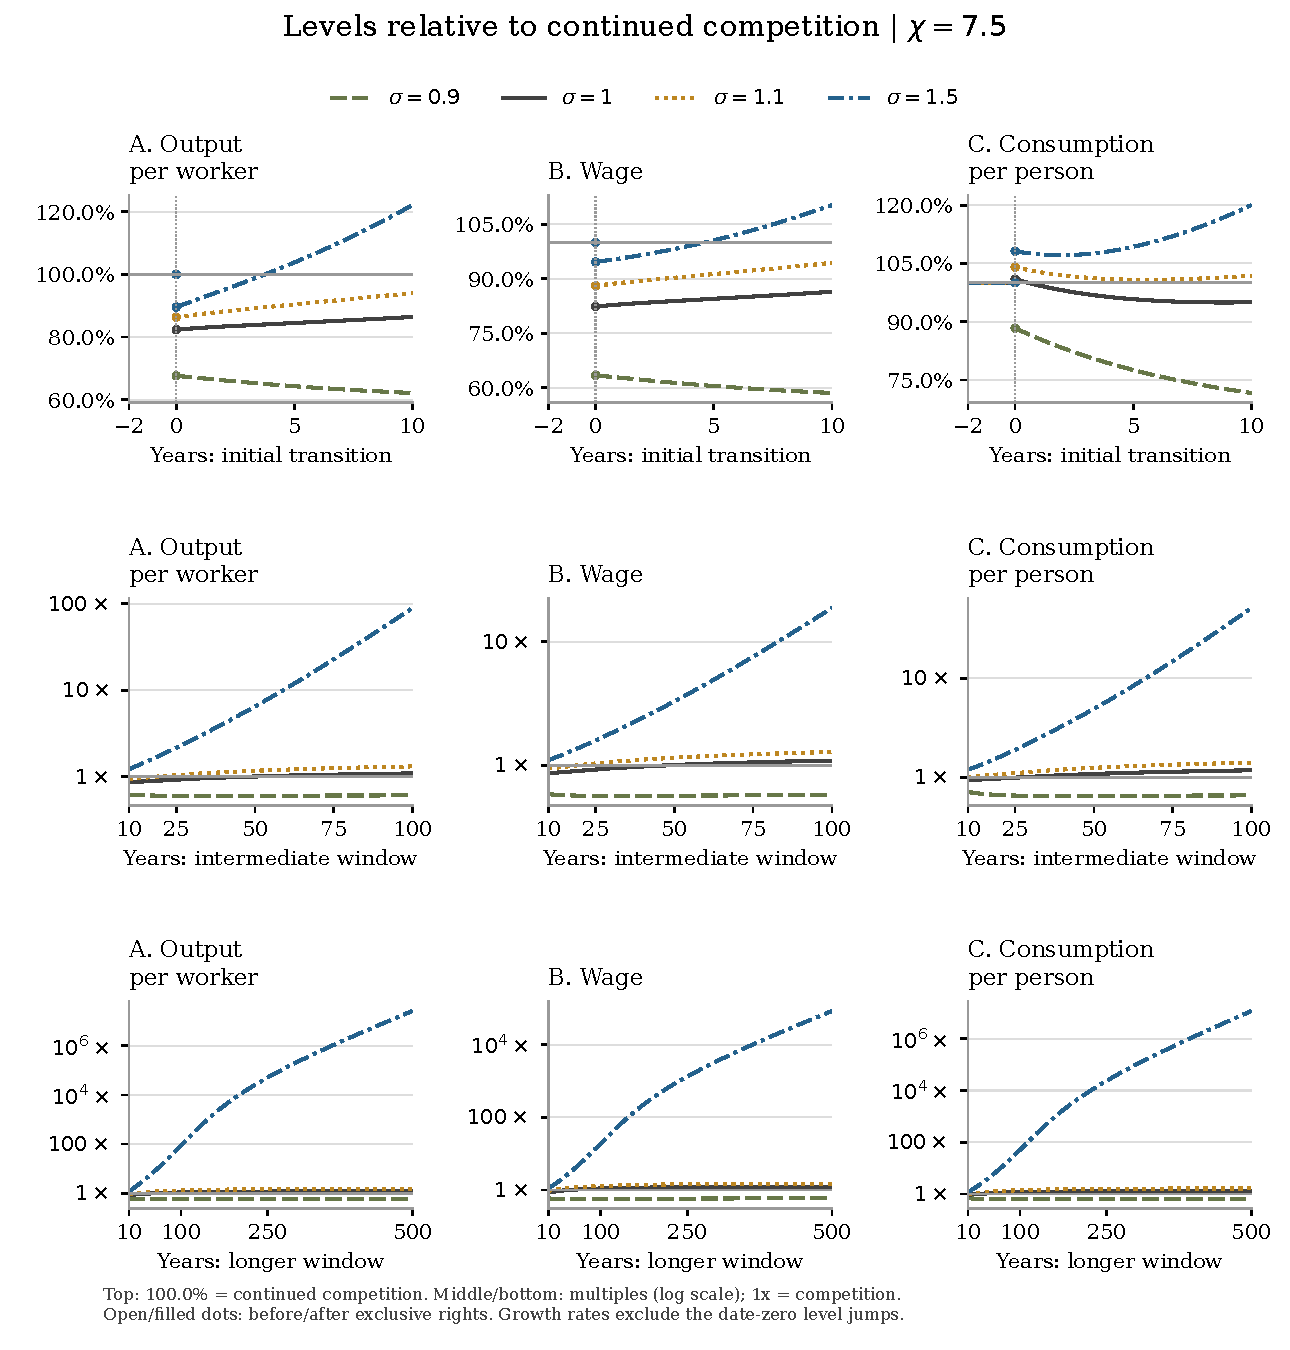
\includegraphics[width=\textwidth]{figures_rewrite/competitive_to_monopoly/competitive_to_monopoly_chi_7_5_levels.pdf}
 \caption{From competition to monopoly with RSI, $\chi=7.5$: levels
 relative to continued competition for all four elasticities. The rows
 cover years $-2$--10, 10--100, and 10--500. The upper row uses percentages;
 the middle and lower rows use multiples on logarithmic scales.
 The horizontal benchmark is $100.0\%$ or $1\times$. Open and filled dots
 mark levels before and after the grant. Vertical scales differ across
 windows and between the two research-productivity exercises.}
 \label{fig:rewrite-competitive-high-levels}
\end{figure}

\begin{figure}[H]
 \centering
 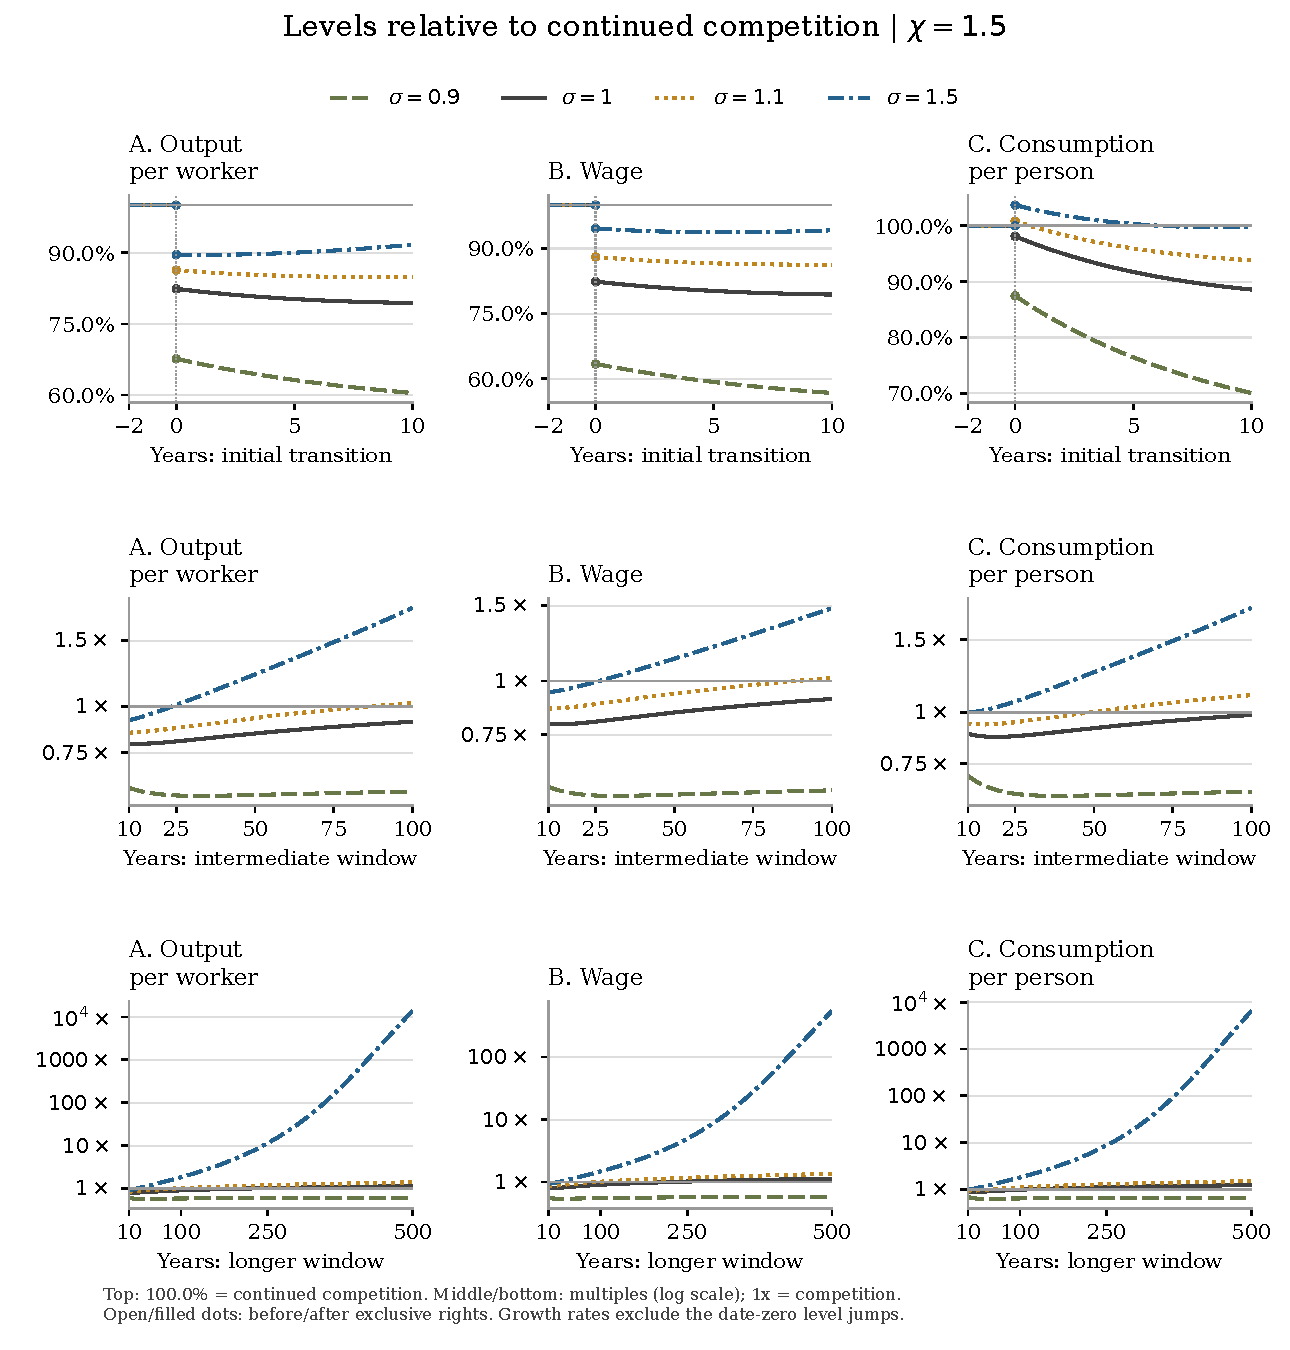
\includegraphics[width=\textwidth]{figures_rewrite/competitive_to_monopoly/competitive_to_monopoly_chi_1_5_levels.pdf}
 \caption{From competition to monopoly with RSI, $\chi=1.5$: output
 per worker, wages, and consumption per person relative to continued
 competition for all four elasticities. Windows, normalizations, and
 line styles match Figure~\ref{fig:rewrite-competitive-high-levels}.
 Vertical scales are fitted to this exercise.}
 \label{fig:rewrite-competitive-low-levels}
\end{figure}

\paragraph{Initial conditions and numerical checks.}
I obtain each competitive initial stock by imposing $r=\rho+\gamma$
with the marginal-cost pricing condition $p_X=1/B_0$. Pre-event
consumption follows from the resource constraint with $M=0$ and
$\dot K=(n+\gamma)K$. The post-event calculation uses the same monopoly
BVP and equilibrium checks as Appendix~\ref{app:rewrite-algorithm}.
Previously computed RSI-activation trajectories supply numerical
initial guesses, but I solve again at the competitive $K_0$, imposing
neither their consumption nor their research choices. All eight
paths pass the same residual, horizon-refinement, transversality,
and developer-optimality checks; no tolerance is relaxed.

\paragraph{Higher research productivity.}
Figures~\ref{fig:rewrite-competitive-high-growth}--\ref{fig:rewrite-competitive-high-distribution}
report $\chi=7.5$. Unlike the pure RSI-activation experiment, the grant
immediately reduces the return on capital: output falls while capital
cannot jump, so equation~\eqref{eq:rewrite-capital-return} implies a
lower interest rate. The Euler equation~\eqref{eq:rewrite-euler}
then gives lower consumption growth immediately after the grant,
even where the level of consumption jumps upward. Subsequent RSI
and capital adjustment determine recovery. Research absorbs resources
before its gains are fully realized, and the distribution panels
separate developer net profit from expenditure on inference and research.

\begin{figure}[H]
 \centering
 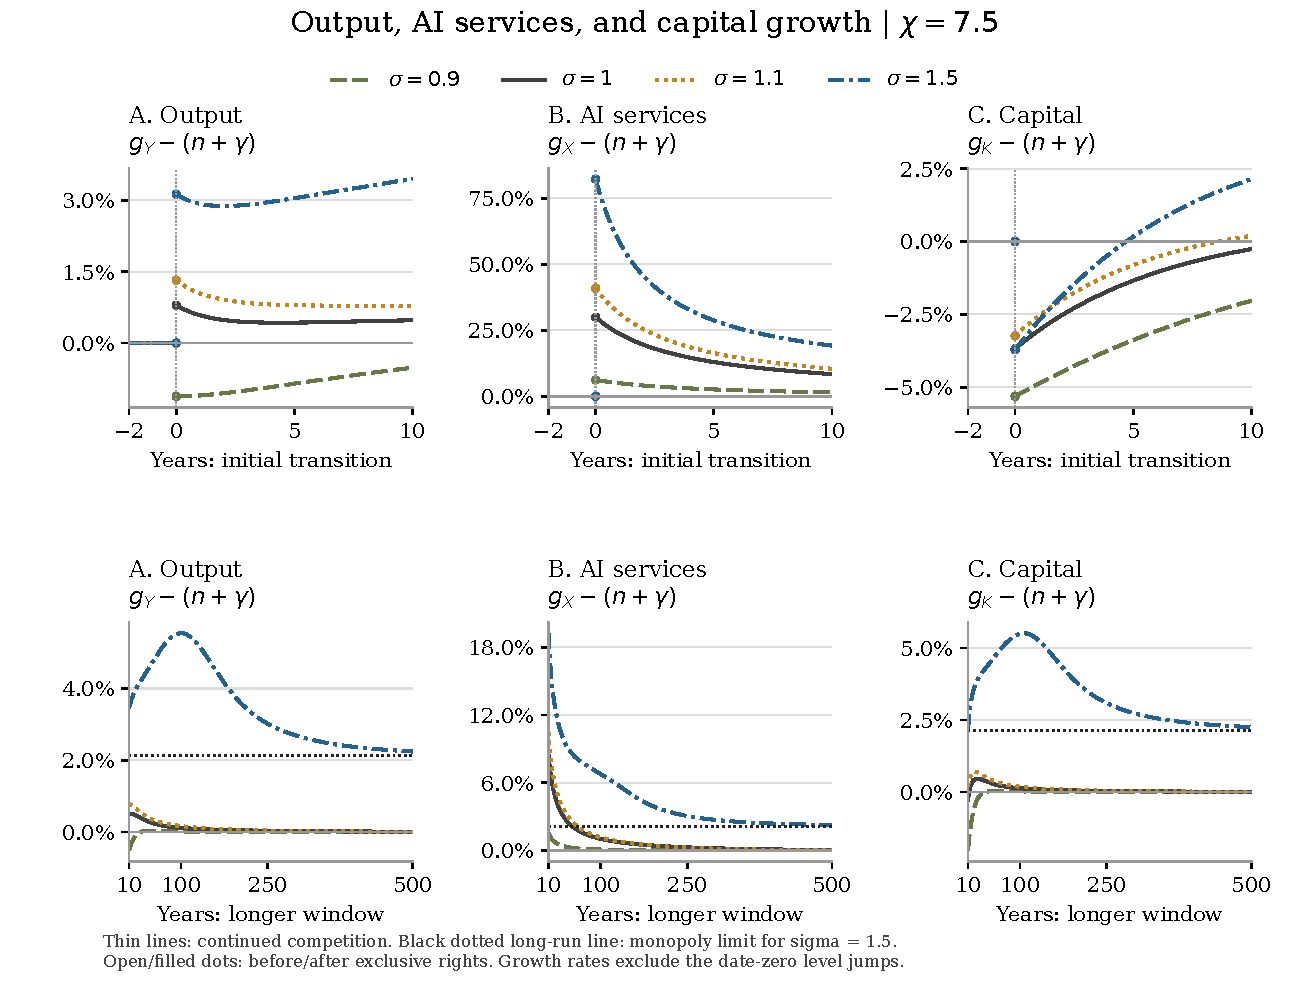
\includegraphics[width=\textwidth]{figures_rewrite/competitive_to_monopoly/competitive_to_monopoly_chi_7_5_accumulation_growth.pdf}
 \caption{Competition to monopoly, $\chi=7.5$: annual growth of output,
 AI services, and capital relative to effective labor. Zero denotes
 growth at $n+\gamma$. Growth rates exclude the discrete level changes
 at date zero.}
 \label{fig:rewrite-competitive-high-growth}
\end{figure}

\begin{figure}[H]
 \centering
 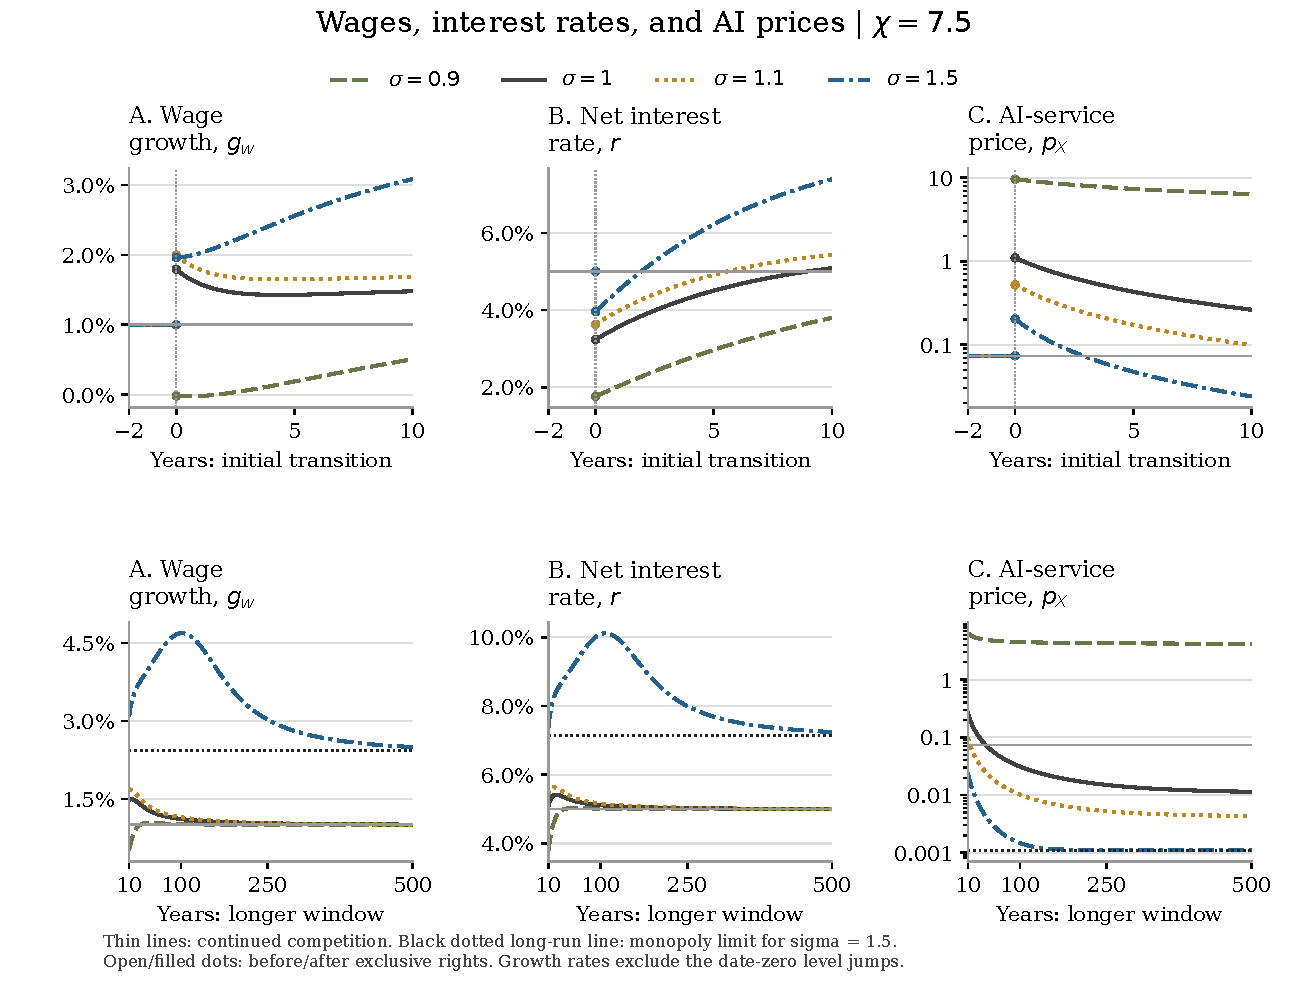
\includegraphics[width=\textwidth]{figures_rewrite/competitive_to_monopoly/competitive_to_monopoly_chi_7_5_growth_returns.pdf}
 \caption{Competition to monopoly, $\chi=7.5$: annual wage growth,
 net interest, and AI-service prices. Prices are measured in final-good
 units on a logarithmic scale. The wage level falls at the grant;
 panel A reports wage growth on either side, not that level change.}
 \label{fig:rewrite-competitive-high-prices}
\end{figure}

\begin{figure}[H]
 \centering
 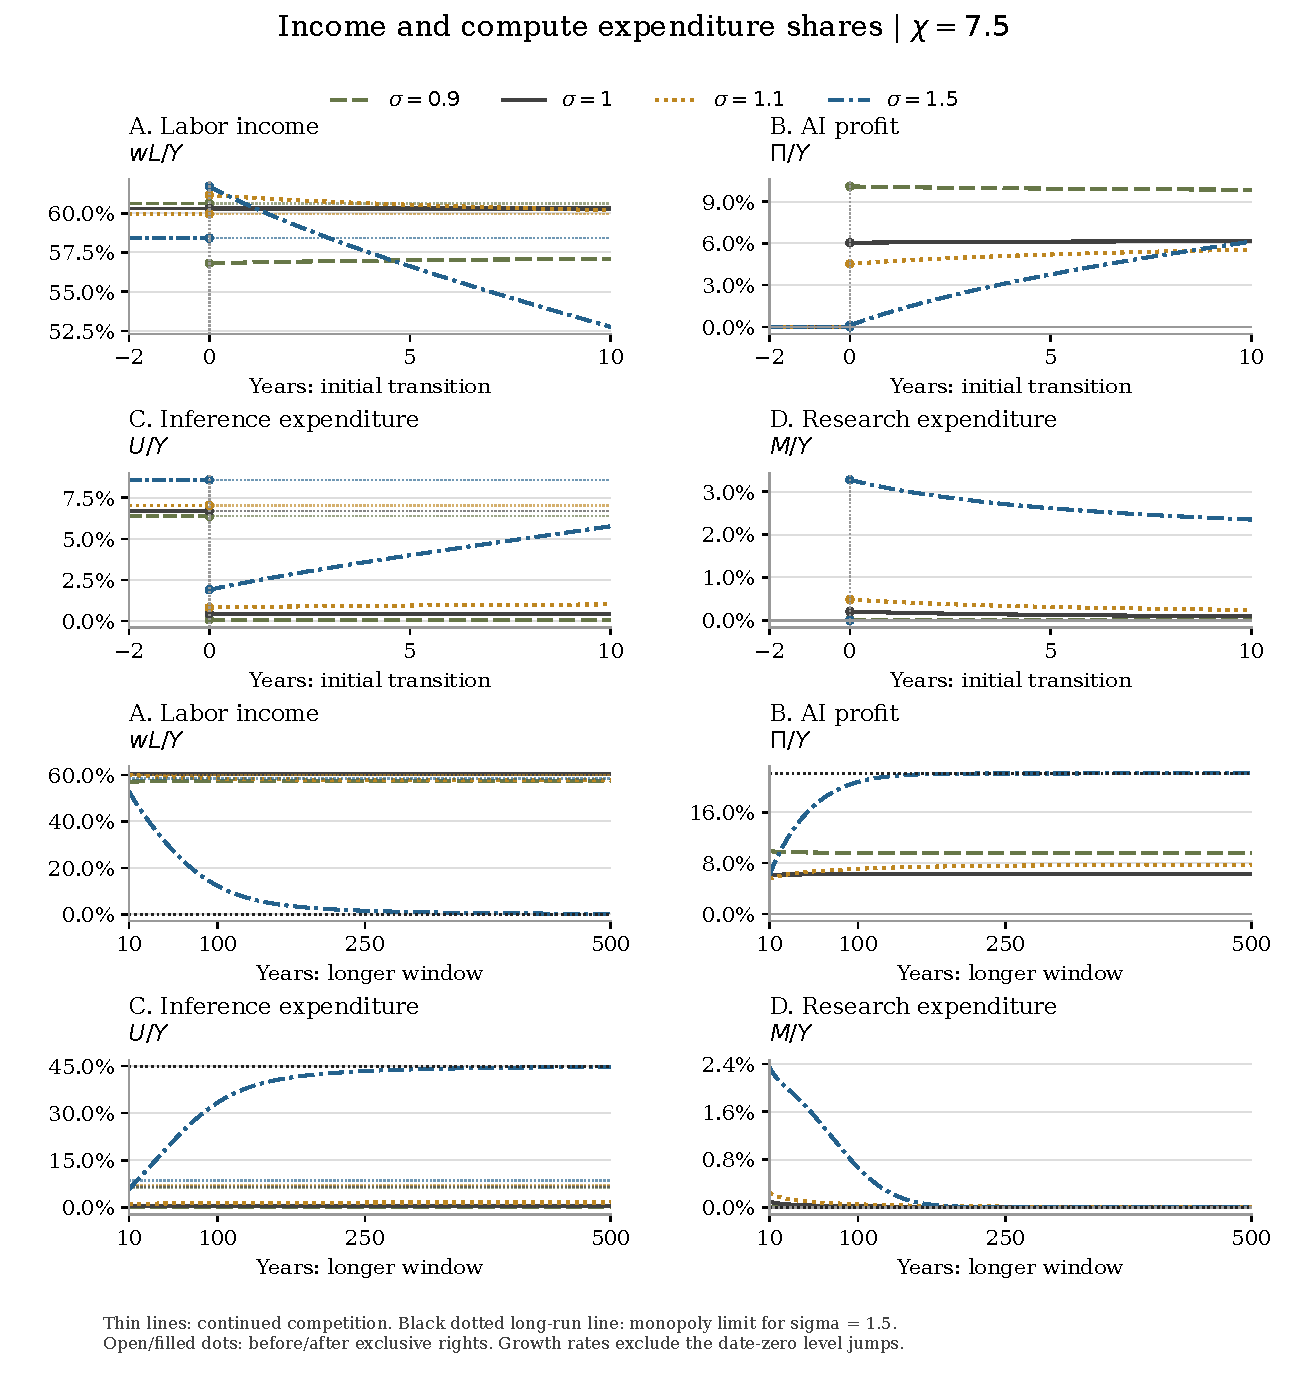
\includegraphics[width=\textwidth]{figures_rewrite/competitive_to_monopoly/competitive_to_monopoly_chi_7_5_distribution.pdf}
 \caption{Competition to monopoly, $\chi=7.5$: labor income, developer
 net profit, inference expenditure, and research expenditure as shares
 of output. The first two rows cover years $-2$--10; the last two
 cover years 10--500. Gross capital income remains $33.0\%$ of output.}
 \label{fig:rewrite-competitive-high-distribution}
\end{figure}

\paragraph{Lower research productivity.}
Figures~\ref{fig:rewrite-competitive-low-growth}--\ref{fig:rewrite-competitive-low-distribution}
report $\chi=1.5$. The impact pricing distortion is unchanged, but
the initial research allocation and efficiency growth are smaller.
At $\sigma=1.5$, the eventual rise in growth and decline in labor's
share emerge later. At year 500, growth and returns still exceed
their monopoly limits, so the final displayed values should not be
read as those limits.

\begin{figure}[H]
 \centering
 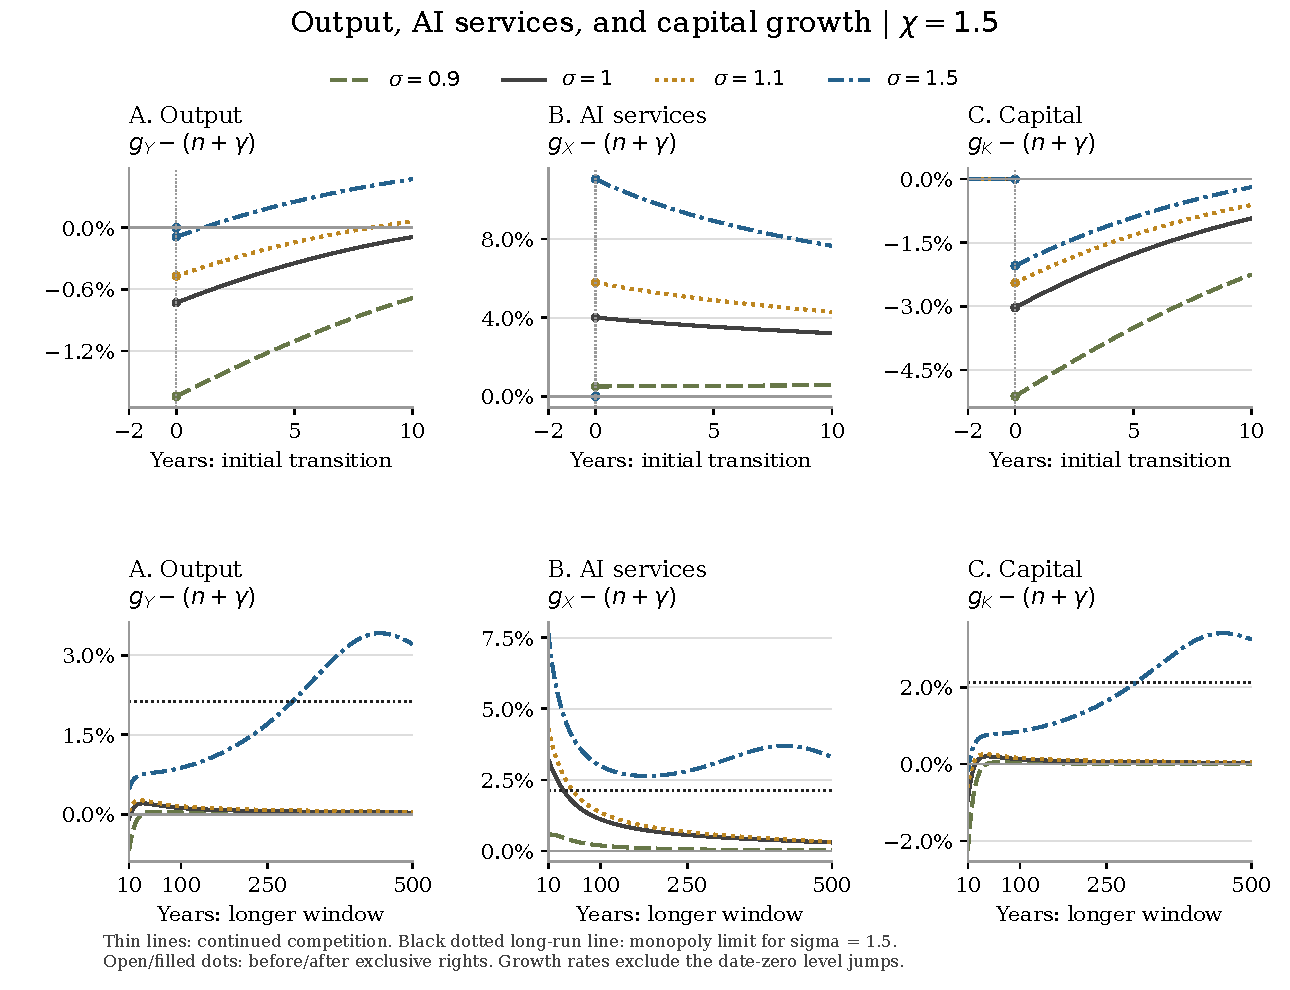
\includegraphics[width=\textwidth]{figures_rewrite/competitive_to_monopoly/competitive_to_monopoly_chi_1_5_accumulation_growth.pdf}
 \caption{Competition to monopoly, $\chi=1.5$: annual growth of output,
 AI services, and capital relative to effective labor. Windows and
 benchmarks match Figure~\ref{fig:rewrite-competitive-high-growth}.}
 \label{fig:rewrite-competitive-low-growth}
\end{figure}

\begin{figure}[H]
 \centering
 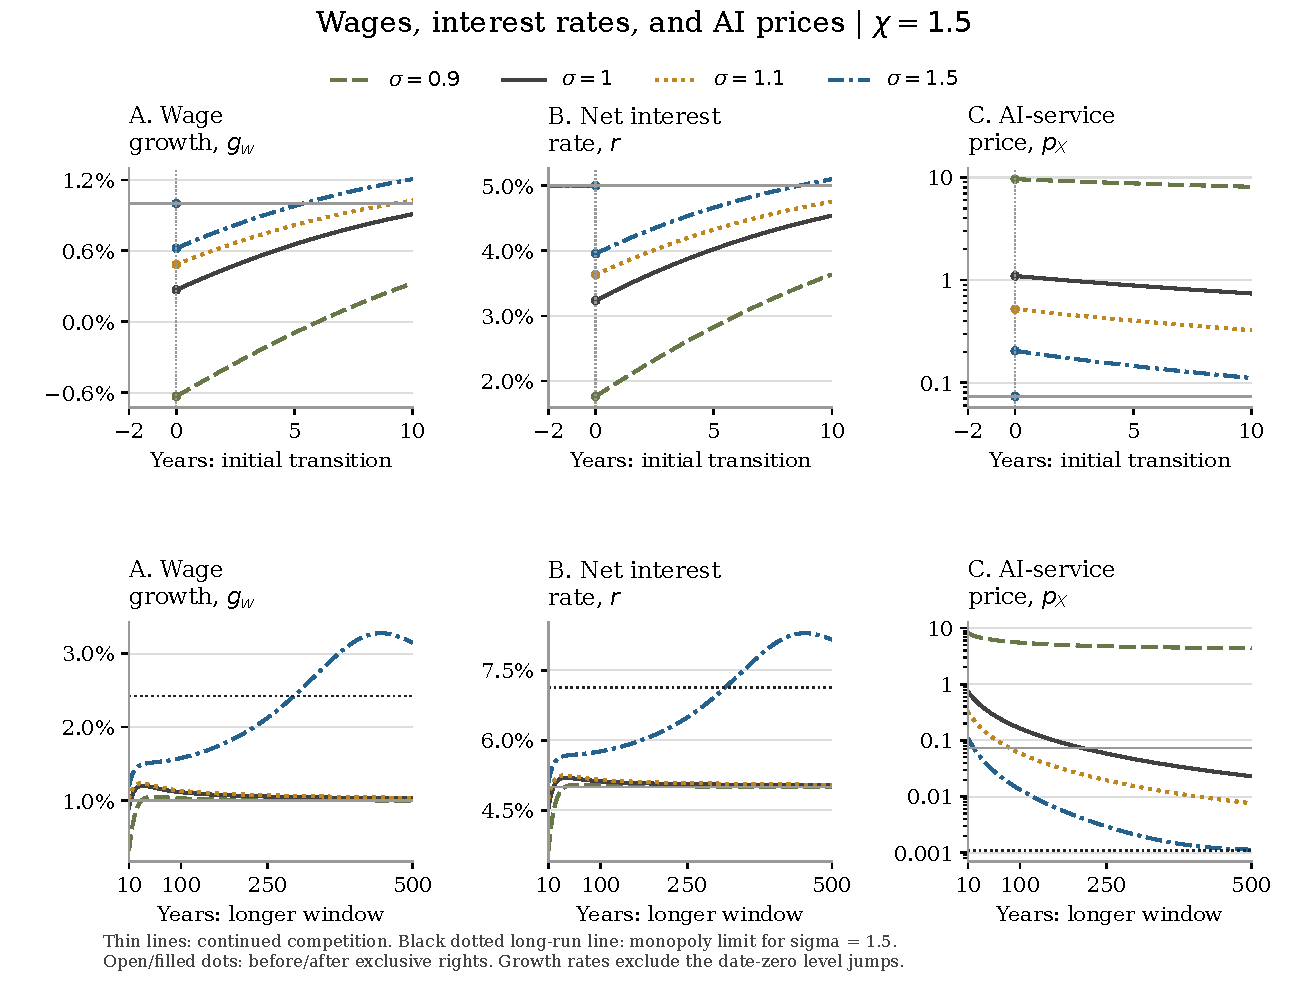
\includegraphics[width=\textwidth]{figures_rewrite/competitive_to_monopoly/competitive_to_monopoly_chi_1_5_growth_returns.pdf}
 \caption{Competition to monopoly, $\chi=1.5$: annual wage growth,
 net interest, and AI-service prices in final-good units. Windows,
 benchmarks, and the logarithmic price scale match
 Figure~\ref{fig:rewrite-competitive-high-prices}.}
 \label{fig:rewrite-competitive-low-prices}
\end{figure}

\begin{figure}[H]
 \centering
 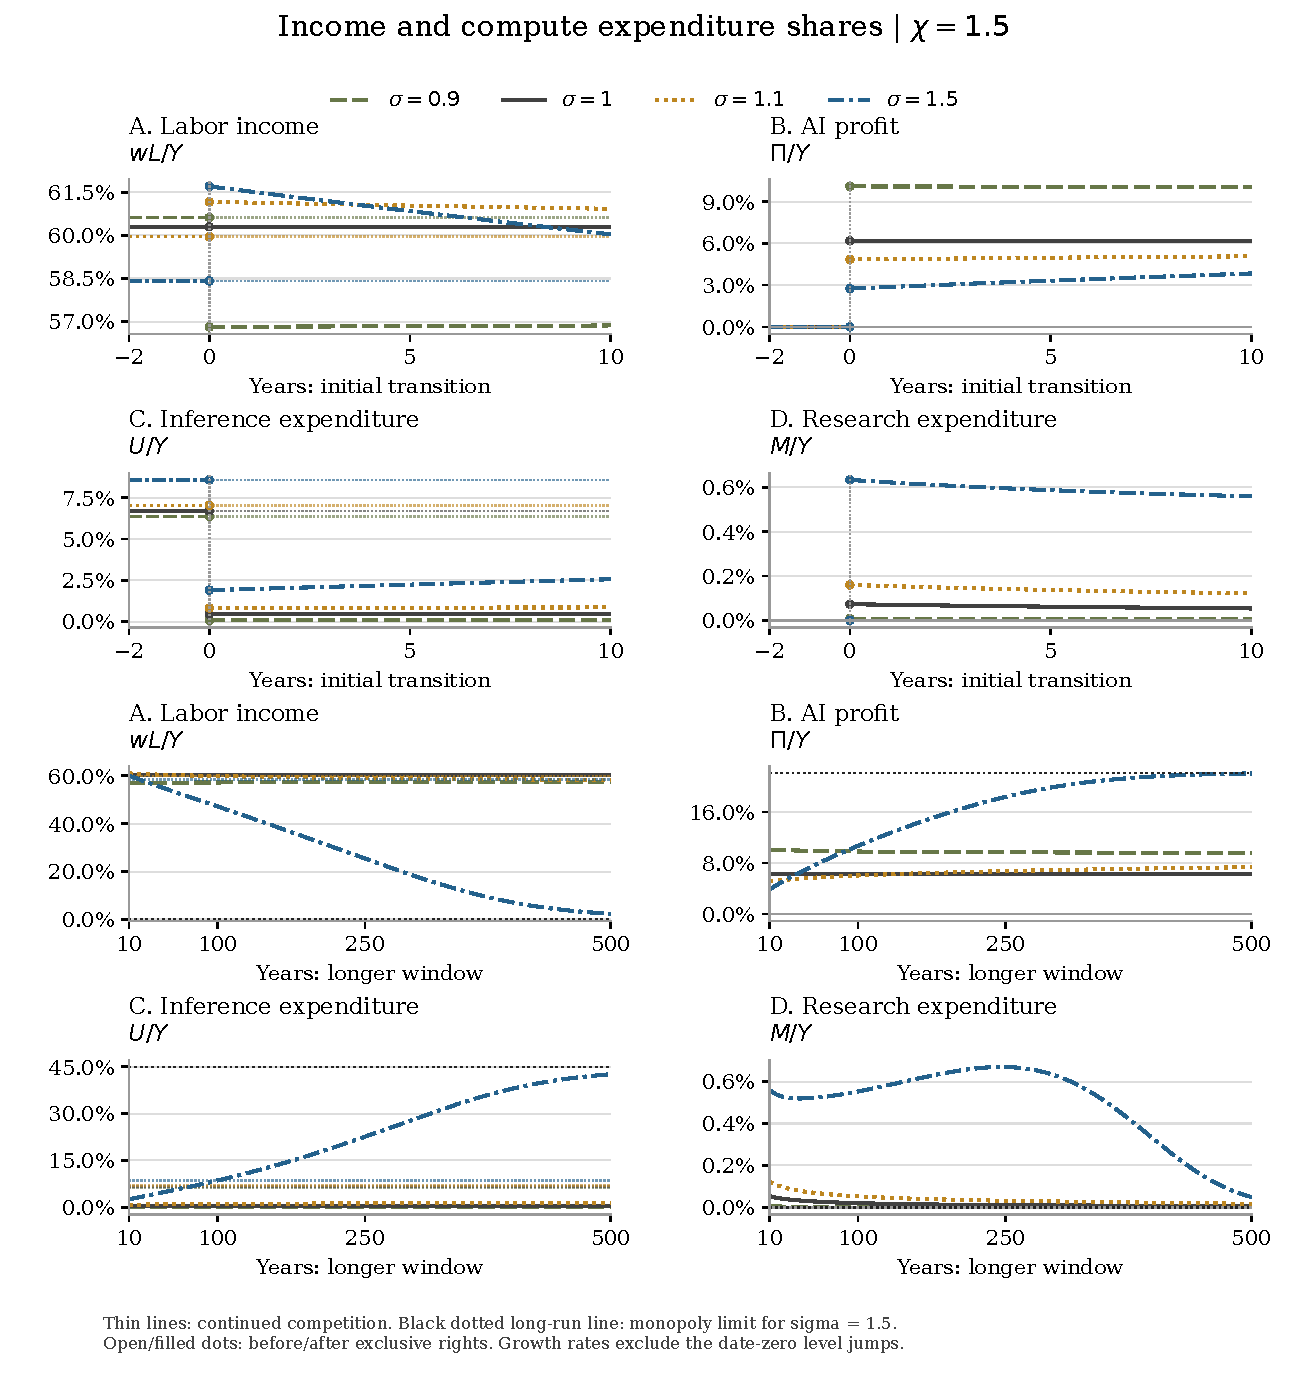
\includegraphics[width=\textwidth]{figures_rewrite/competitive_to_monopoly/competitive_to_monopoly_chi_1_5_distribution.pdf}
 \caption{Competition to monopoly, $\chi=1.5$: labor income, developer
 net profit, inference expenditure, and research expenditure relative
 to output. Layout and benchmarks match
 Figure~\ref{fig:rewrite-competitive-high-distribution}.}
 \label{fig:rewrite-competitive-low-distribution}
\end{figure}

\paragraph{Replication.}
The repository's
\href{https://github.com/oliverpardo1979/ai-growth-and-labor/blob/main/COMPETITIVE_TRANSITION.md}
{competitive-transition guide} records the parameters, the institutional
experiment, and the replication commands. The driver is
\path{scripts/simulate_competitive_to_monopoly.py}; the renderer is
\path{scripts/report_competitive_to_monopoly.py}.
The guide links to the separate results folders for each research
productivity, containing the original paths, competitive benchmarks,
impact changes, and numerical audits.
The main-text $\sigma=1.5$ comparison is rendered by
\path{scripts/report_competitive_main_comparison.py}, which reads these
same audited paths without changing them.
Figure windows only select dates from those stored paths; they do not
change the simulated economy or the numerical solution horizon.

The repository's
\href{https://github.com/oliverpardo1979/ai-growth-and-labor/blob/main/MONOPOLY_GROWTH_REVERSAL.md}
{growth-reversal replication guide} records the separate input choices,
data, audit reports, and commands. The original growth-reversal
experiment, initialized at $A_0=N_0=1$, remains archived in separate
files; the other simulation exercises are unchanged.

\paragraph{Growth reversal under exclusive rights.}
For Section~\ref{subsec:rewrite-monopoly-growth-reversal}, I first
construct a competitive prehistory with $B=B_0$ above the competitive
threshold. At the start of this prehistory, I normalize $A=N=1$ and
set $K=14{,}047.3$, the limiting monopoly capital--effective-labor ratio
at the chosen upper bound. These seed values are illustrative; they
are not the stocks at the monopoly grant. I advance the competitive
path to year 190, the first whole year at which the three rates in
\eqref{eq:rewrite-competitive-ai-growth} are each within 0.1 percentage
point of their limits; all subsequent annual observations through
year 1,000 also satisfy this criterion. I then set that date to zero
and inherit $A$, $N$, and $K$ without changing units. Re-solving the
competitive equilibrium from those stocks reproduces the continued
prehistory path to within $10^{-9}$ in log levels over the next 500
years. The figures include its last ten pre-grant years.

I solve the competitive
resource constraint and Euler equation in
\eqref{eq:rewrite-competitive-normalized}, with $M=0$ and $B=B_0$,
using the inherited capital stock and the terminal condition
$C/K\to\rho-n$ from
\eqref{eq:rewrite-competitive-capital-growth}.
The numerical coordinates are $\log(C/K)$ and
$\log(K/(AL))-[\mathcal R^{\mathrm{mc}}(B_0)-\rho-\gamma]t$.
Removing the limiting trend avoids extremely large levels without
imposing balanced growth on the transition. I use the same
\texttt{scipy.integrate.solve\_bvp} routine described in the numerical
appendix. Extending its horizon from 1,200 to 1,800 years changes
these coordinates by less than $10^{-9}$ over the displayed 500 years;
independent finite-difference residuals are below $10^{-9}$.
The static supply condition, positive allocation, limiting growth
rates, and household transversality diagnostics also pass the checks.

I solve the two monopoly paths using the existing continuation method,
without changing its equilibrium-admission tolerances. Their final
solution horizon is about 4,592 years, although the figures display
only the first 500 years. Both pass the equation, horizon-extension,
transversality, and developer-optimality checks, including denser
checks over the first decade.


\section*{Declaration of AI use}
During the preparation of this work, I used OpenAI Codex to assist with mathematical derivations, consistency checks, manuscript editing, and the preparation and testing of computational code. I take full responsibility for the content of the paper.

\bibliographystyle{apalike}
\phantomsection
\addcontentsline{toc}{section}{References}
\bibliography{references}

\end{document}
